%%%%%%%%%%%%%%%%%%%%%%%%%%%%%%%%%%%%%%%%%%%%%%%%%%%%%%%%%%%%%%%%%%%%%%%%%%%%%
%
% This is a template CEPC Paper that contains suggestions and hints on
% how to get your note in a form that minimizes the amount of work
% needed to get it approved by the collaboration - assuming that the
% physics is OK!
%
%%%%%%%%%%%%%%%%%%%%%%%%%%%%%%%%%%%%%%%%%%%%%%%%%%%%%%%%%%%%%%%%%%%%%%%%%%%%%%

%\documentclass[11pt,a4paper]{cepcnote}
\documentclass[coverpage]{cepcnote} 
\graphicspath{{figures/}}
\usepackage{cepcphysics}
\usepackage{subfigure}
\usepackage{mathrsfs}
\usepackage{authblk}
\usepackage{amsmath, amssymb}
\usepackage{slashed}
\usepackage{multirow}
\usepackage{lineno}
%\newcommand{\bslash}{\ensuremath{\backslash}}
\def\Slash#1{\!\not\!\! #1}             % Feynman dagger for upper case
\def\slash#1{\!\not\! #1}               % Feynman dagger for lower case
\newcommand{\etmiss}{\ensuremath{\slashed{E}_T}} %added by baiyu
\newcommand{\emiss}{\ensuremath{\slashed{E}}}    %added by baiyu
\newcommand{\mmiss}{\ensuremath{\slashed{M}}}    %added by baiyu
\newcommand{\mmissquare}{\ensuremath{\slashed{M}^2}} %added by baiyu

\newcommand{\minitab}[2][l]{\begin{tabular}{#1}#2\end{tabular}}  %added by baiyu
\renewcommand{\multirowsetup}{\centering}       %added by baiyu
\newcommand{\tabincell}[2]{\begin{tabular}{@{}#1@{}}#2\end{tabular}} %added by baiyu

%font size
\newcommand{\zhonghao}{\fontsize{10pt}{\baselineskip}\selectfont}
\newcommand{\chuhao}{\fontsize{8pt}{\baselineskip}\selectfont}
\newcommand{\xiaochuhao}{\fontsize{5.4pt}{\baselineskip}\selectfont}
\newcommand{\xiaohao}{\fontsize{5.0pt}{\baselineskip}\selectfont}

%%% commands Alex
\newcommand{\inmath}[1]{\ensuremath{#1}\xspace}
%\newcommand{\eg}{e.\,g.\@\xspace}
%\newcommand{\Eg}{E.\,g.\@\xspace}
%\newcommand{\ie}{ie\@ifnextchar.{}{.\@}}
%\newcommand{\Ie}{I.\,e.\@\xspace}
\newcommand{\percent}[1]{{#1}\,\%}
\newcommand{\todo}[1]{{\color{red}TODO: #1}}
\newcommand{\metx}{\inmath{\met}}
\newcommand{\meffx}{\inmath{m_\text{eff}}}
\newcommand{\mttwox}{\inmath{m_\text{T2}}}
\newcommand{\summtx}{\inmath{m_T(\lepton_1) + m_T(\lepton_2)}}
\newcommand{\mctx}{\inmath{m_\text{CT}}}
\newcommand{\Wjetsx}{$W$~+ jets\xspace}
\newcommand{\Zjetsx}{$Z$~+ jets\xspace}
\newcommand{\ttbarx}{\ttbar\xspace}
\newcommand{\ptx}{\pt\xspace}
\newcommand{\Table}[1]{Table~\ref{#1}\xspace}
\newcommand{\Fig}[1]{Figure~\ref{#1}\xspace}
%\newcommand{\GeV}[1]{\unit[#1]{GeV}\xspace} % I made sure no one is using \GeV before adding this line
\newcommand{\ifbx}[1]{\unit[#1]{\ifb}\xspace}
\newcommand{\eighttev}{\inmath{\sqrt{s} = \unit[8]{TeV}}}
\newcommand{\com}{\inmath{\sqrt{s} = \unit[250]{GeV}}}
\newcommand{\lumiunit}{\ensuremath{\mathrm{cm}^{-2}\mathrm{s}^{-1}}
}
\makeatletter
\DeclareRobustCommand*{\trigger}[1]{%
  \begingroup\@activeus\scantokens{#1\endinput}\endgroup}
\begingroup\lccode`\~=`\_\relax
   \lowercase{\endgroup\def\@activeus{\catcode`\_=\active \let~\_}}
\makeatother
\newcommand{\neutralinon  }[1]{\inmath{\widetilde{\chi}_{#1}^0}}
\newcommand{\charginon    }[1]{\inmath{\widetilde{\chi}_{#1}^\pm}}
\newcommand{\taupll       }{tau~+ light lepton\xspace}
\newcommand{\lepton       }{\ensuremath{\ell}}
\newcommand{\nnh          }{\ensuremath{\nu \bar{\nu} H} }
\newcommand{\llh          }{\ensuremath{l^{+}l^{-}H}}
\newcommand{\eeh          }{\ensuremath{e^{+}e^{-}H}}
\newcommand{\mmh          }{\ensuremath{\mu^{+}\mu^{-}H}}
\newcommand{\tautauh      }{\ensuremath{\tau^{+}\tau^{-}H}}
\newcommand{\qqh          }{\ensuremath{q\bar{q}H}}
\newcommand{\bpair           }{\ensuremath{b\bar{b}}}
\newcommand{\cpair           }{\ensuremath{c\bar{c}}}
\newcommand{\gpair           }{\ensuremath{gg}}
\newcommand{\qpair           }{\ensuremath{q\bar{q}}}
\newcommand{\leppair           }{\ensuremath{l^{+}l^{-}}}
\newcommand{\leppm             }{\ensuremath{l^{\pm}}}
\newcommand{\lepmp             }{\ensuremath{l^{\mp}}}
\newcommand{\elpair           }{\ensuremath{e^{+}e^{-}}}
\newcommand{\elpm             }{\ensuremath{e^{\pm}}}
\newcommand{\elmp             }{\ensuremath{e^{\mp}}}
\newcommand{\mupair           }{\ensuremath{\mu^{+}\mu^{-}}}
\newcommand{\mupm             }{\ensuremath{\mu^{\pm}}}
\newcommand{\mump             }{\ensuremath{\mu^{\mp}}} 
\newcommand{\taupair           }{\ensuremath{\tau^{+}\tau^{-}}}
\newcommand{\taupm             }{\ensuremath{\tau^{\pm}}}
\newcommand{\taump             }{\ensuremath{\tau^{\mp}}}
%\newcommand{\ten          }[1]{\cdot 10^{#1}}
\newcommand{\ten           }[2]{\ensuremath{{#1}\times 10^{#2}}}
%%%

% Shorthand for \phantom to use in tables
\newcommand{\pho}{\phantom{0}}
\newcommand{\bslash}{\ensuremath{\backslash}}
\newcommand{\BibTeX}{{\sc Bib\TeX}}

%%%%%%%%%%%%%%%%%%%%%%%%%%%%%%%%%%%%%%%%%%%%%%%%%%%%%%%%%%%%%%%%%%%%%%%%%%%%%%
% Preamble
%%%%%%%%%%%%%%%%%%%%%%%%%%%%%%%%%%%%%%%%%%%%%%%%%%%%%%%%%%%%%%%%%%%%%%%%%%%%%%

%\title{ Higgs Mass and Cross-section Measurement at CEPC }
\title{Measurement of $H\to \bpair /\cpair /\gpair$ Branch Ration from $ZH$ Production with  $\nnh$, $\llh$ and $\qqh$  Final States in CEPC Experiment}
%\title{A template for CEPC papers}
\author{CEPC Workgroup}
\mail  {baiy@seu.edu.cn}
%\draftversion{1.0}
\cepcnote{CEPC\_ANA\_HIG\_2016\_XXX}
\abstracttext{
  
%  This is a template CEPC paper. It contains the structure, style
%  files and hints on how to produce a paper for which a minimum amount
%  of time is necessary to spend on typographic details. This template
%  can be found on the web pages of the CEPC Collaboration. 
%  You can find some \LaTeX{} technical detail about the
%  template in the Appendix of this paper.
  A couple of remarks about the paper front page:
  \begin{itemize}

  \item {\bf Title:} Measurement of $Hboson\to \bpair /\cpair /\gpair$ Branch Ration from $ZH$ Production with \nnh, \llh and \qqh  Final States in CEPC Experiment
  \item {\bf Author list:} it will be provided by the CEPC Collaboration,
    and will be made available on their website. On the
    front page, you should name ``The CEPC Collaboration'' as
    author.

  \item {\bf Abstract:}
  A study on the measurement on $Hboson\to \bbbar /\ccbar/gg$ branch ratio, one of the benchmark measurements in CEPC experiment, is presented here. In the scenario concerned, the Higgs boson are produced associated with a Z boson,
  and subsequently undergo hadronic decay, while the $Zboson$ decays to neutrino pair, charged lepton pair or quark pair.  

%  This analysis,in complementary with the measurement on other states of ZH production, can be used to derive the Yakawa coupling, one of the key properties to understand the Electroweak symmetry breaking mechanism. \par
   An integral luminosity of 5000 fb$^{-1}$ is assumed to estimate the signal and background yielding, corresponding to 10 years running of CEPC with nominal luminosity at \ten{2}{34} $\lumiunit$. A cut based analysis is applied to each analysis, combined with multi-variable method. The flavor information in final states 
   are extracted by fitting each flavor components according to their templates. A Toy Monte-Carlo test was done to evaluate the statistic uncertainty. 
   They systematic uncertainty was also disccussed and estimated.
   We conclude the measurement of $\Hboson \to \bpair/\cpair/\gpair$ reach the precision \percent{0.2}, \percent{2} and \percent{3}. 
   %A cut based analysis gives xxx signal events and xxx.xxx background events. The flavor components was distinguished using a template fit method. In addition study of various of technics such as TMVA, tag counting are on going.
%    it should also be clear, descriptive, and
%    concise. It should ideally be one paragraph long, and certainly no
%    more than half a page. It should stand on its own and, similarly,
%    the main text of the paper should not depend on it. The abstract
%    should state: what was the measurement; where was it done and with
%    what dataset/luminosity; what method was used; what are the
%    primary results and main conclusions.  Citations in an abstract
%    should be avoided. If only Monte Carlo data are used in the
%    publication, this fact should be stated explicitly in the
%    abstract.  
    
  \end{itemize}
}

%%%%%%%%%%%%%%%%%%%%%%%%%%%%%%%%%%%%%%%%%%%%%%%%%%%%%%%%%%%%%%%%%%%%%%%%%%%%%%%
% This is where the document really begins
%%%%%%%%%%%%%%%%%%%%%%%%%%%%%%%%%%%%%%%%%%%%%%%%%%%%%%%%%%%%%%%%%%%%%%%%%%%%%%%

\begin{document}
\linenumbers
\tableofcontents
\clearpage

\section{Introduction}\label{sec:introduction}
The discovery of a scalar boson with mass around 125 \GeV at LHC \cite{Higgs_ATLAS, Higgs_CMS} completed the final piece of the standard model.
This particle, interpreted as the Higgs boson, plays a crucial role in the electroweak spontaneous symmetry broken (EWSB), 
known as the BEH (Brout-Englert-Higgs) mechanism \cite{BEH,BEH2,BEH3}, often referred as the Higgs mechanism.
The higgs meachism allows the $\Wboson$, $\Zboson$, 
quarks and charged leptons to be massive while keeping the $SU(2)_L \times U(1)_Y$ gauge invariance.
The Higgs mechanism allows the $\Wboson$, $\Zboson$, quarks and charged leptons to be massive while keeping the $SU(2)_L \times U(1)_Y$ gauge invariance. The masses of the SM fermions ($m_{f_i}$) in the SM are proportional to their Yukawa couplings ($h_i$) to the Higgs field: $m_{f_i} = \dfrac{vh_i}{\sqrt{2}}$, where $v\approx 246\GeV$ is the vacuum expectation value of the Higgs field (VEV).

Measuring the Yukawa couplings between higgs and SM fermions is essential to undertand the origin of the fermions' masses and the detail of EWSB.
The dominant direct higgs decays into fermionic final states are $\Hboson\to \bpair$, $\Hboson\to\cpair$ and $\Hboson\to\taupair$, 
the decay branching ratios of which are estimated to be \percent{57}, \percent{4} and \percent{3}. 
In addition, the Higgs boson can decay to gluon pairs via a heavy quark loops. The large coupling between higgs and top quark leads to considerably large 
branching ratio of $\Hboson\to\gpair$ that is estimated to be about \percent{9}. 
\par
Until now, the LHC is the collider to directly study the Higgs mechansim. 
The leading higgs fermionic decay,  $\Hboson\to\bpair$ was studied in both ATLAS and CMS experiment in VH\cite{VH_bb_atlas,VH_bb_cms}, ttH\cite{ttH_bb_cms} and VBF\cite{VBF_bb_atlas,VBF_bb_cms} process, with the LHC Run-I data.
The combination of ATLAS and CMS gives $\bpair$ $\sigma\times Br$ signal strength for $0.70\pm0.29$ in run-I data\cite{higgs_atlas_cms_combine}. 
A study on $\Hboson\to\bpair$ in which Higgs are produced in association with $W$ or $Z$ boson, using \ifb{36.1} Run-II data with center of mass 13 TeV in ATLAS, 
constrained the signal strength as $1.20^{0.24}_{-0.23}(stat.)^{+0.34}_{-0.28}(sys.)$ \cite{VHbb_atlas_run2} with 3.5 $\sigma$ signal significance.
The large uncertainty is due to huge QCD or vector boson production with muliti-jets backgrounds, which is inevitable in hadron colliders. 
\par
%The Circular Electron Positron Collider(CEPC) \cite{CEPC_preCDR} program is proposed with the goal to better understand the EWSB
% by precisely measuring on these higgs parameters as well as other EW parameters of interest. 
% The CEPC has the advantages in precision measurement:
% \begin{itemize}
% \item Clean backgrounds
% \item Well defined frame of center momentum
% \item High luminosity
% \end{itemize}
On the other hand, with much fewer background events and well defined initial and final states, the proposed Circular Electron Positron Collider (CEPC)~\cite{CEPC_preCDR} 
will have capability to carry out precision measurements of many Higgs decay modes that are inaccessible at the LHC.
% The center of mass enerey is configured as \GeV{250}, well above the $\Zboson\Hboson$ threshold.
% With the nominal luminosity at \ten{2}{34}\cm2s1, \ifb{5000} data can be accumulated in ten years of running. 
% Over one million higgs boson will be produced. Clean background and high statistics make precise measurement possible.
%The outline of higgs background will be discussed in section \ref{sec:CEPC_MC}
%\par
%The works presented in this note demostrate the capability of the $\Hboson \to \bpair/\cpair/\gpair$ measurements in CEPC.
%The higgs productions associate with charged lepton(electrons or muons) pair, neutrino pair or quark pair are studied.
% In Section II, a brief introduction of CEPC experiment and the MC sample will be presented. In section III the event selection and the analysis strategy will be described. In section IV the results are listed and discussed. Detail information, auxiliary figures, tables and numbers, as well as analysis method in study can be found in appendix.
%\par
The studies presented in this note demonstrate the capability to perform precision measurements of the Higgs boson decay branching ratio in the $\bpair$,$\cpair$ and $\gpair$ final states 
at the CEPC. We consider the Higgs boson production mainly in association with a $Z$ boson, where $Z$ is reconstructed in the $\nu\bar{\nu}$, $ell\ell$ and $\qpair$ final states.
This note is organized as follows: section II gives a brief introduction of the CEPC and MC samples used in the analysis; section III focuses on the analysis detail including event selection 
of the $\llh$, $\nnh$ and $\qqh$ channel; in section IV, flavor tagging issues will be described, including the tagging techniques and template fit method; in section V, the validation to 
the template fit will be discussed; in section VI and VII, the results and conclusion will be presented.
\clearpage

\section{CEPC Experiment and MC Sample}
\label{sec:CEPC}
\subsection{CEPC experiment}
The CEPC is a future ciruclar electron-positron collider project. Two detectors will be installed at two interaction 
points in the stoarge ring, 50-100 kilometers in circumference. Electrons and positrons collide at each interaction point with center of mass energy 240 - 250 GeV. The luminosity is design to be \ten{2}{34} \lumiunit.
 The higgs boson are produced mainly via associated production with Z boson(96.6\%) as well as much $WW$ fusion (with $\nu_e\bar{\nu}_e H$ in final states,3.06\%) and $ZZ$ fusion(0.29\%, with $e^+e^-H$ in final state).
 
\cite{CEPC_preCDR}. 

\subsection{CEPC detector}
A ILD-like detector is designed as the CEPC detector(CEPC-v1) with additional considerations\cite{CEPC_preCDR}. Detail description of ILD model can be found in \cite{ILD_detector}. All changes need to be implemented into simulation, and iterate with physics analysis and cost estimation.

\subsection{MC Samples}
In this analysis, the signal events are $e^+e^-\to \Zzero \Hboson\to\qqbar + \bbbar/\ccbar/gg$. The standard model background includes di-quark events, di-lepton events, vector boson pair production and higgs production with final states different from the signal. Both background and signal events are generated using Whizard\cite{Wizard_1} with assumption of collision by no-polarization electron-positron, with center of energy of 250 GeV. PHYTHIA 6.4 \cite{PYTHIA64} was used to model the fragmentation and hadronization. The higgs mass was assumed to be 125 GeV and the coupling was set as that predicted by standard model.\par
The generated signal events and backgrounds events with higgs production undergo the GEANT4\cite{Geant4} based detector simulator Mokka\cite{mokka} with CEPC-v1. The simulated hits were digitized and reconstructed by the MarlinReco package. 
%The  LCFIPlus\cite{LCFIPlus} toolkit was utilized to reconstruct the primary vertex, jets and secondary vertex. 
The jets are reconstructed with Durham-like algorithm\cite{Durham} by implementing the toolkit lcfiplus\cite{LCFIPlus}. This toolkit is also capable to reconstruct the primary and secondary vertex, as well as jet flavor tagging.\par
Background events without higgs production undergo fast simulation, which includes:
\begin{itemize}
\item Four momentum of jet(b,c quarks and gluon) is smeared according to a Gaussian function, with jet energy  
resolution $\sigma$ set to be 4\%.
\item Each leptonic track ($e/\mu$) is corrected by momentum resolution and tracking efficiency, whose parameter are obtained from the study of the full simulation.
\item The four momentum of neutrino decaying from the final hadron subtracted from the four momentum of jet.
\end{itemize} 
The fast simulation reconstruct jets using a simplified algorithm. It is faster but with disadvantage that the vertex information is missing from reconstruct. Full simulation sample of the backgrounds are also in production and results will be updated using those samples. Detailed information of MC samples can be found in \cite{Samples}.
\clearpage

\section{Analysis Strategy and Event Selection}\label{sec:event_selection}
Two steps of analysis are taken. In the first step, a series of object and event selection was applied to maximize the sensitivity to detect the signal; in the second step,  a template fit on the 2-Dimension flavor weight distribution, which is got from TMVA based flavor tagging algorithm, is implemented to further distiguish the flavor components in final states. The details of template fit are described in \ref{sec:templatefit}.\par
The final states with 2 jets, 2 jets + 2 leptons(either electron or muon pair), 4 jets are required for \nnh,\llh and \qqh channel respectively.
\par
\subsection{$\llh$ Event Selection}
The $\llh$ channel is the composite of two sub-channels of $\eeh$ and $\mmh$ process. The dominant backgrounds are semi-leptonic $ZZ$ process and other $ZH$ production followed by other types of higgs decay(mainly by higgs decay to off-shell $W$ or $Z$ pair, and both intermediate boson undergo hadronic decay).
Two isolated tracks with opposite charge, reconstructed as electrons or muons, are required in addition to a pair of jets.  The recoil mass provide a very clear signature of the signal events, which have been delicately studied in \cite{CEPC:recoilmass}. 
The cut criteria of lepton pair recoil mass, together with the invariant mass of jet pair and lepton pair, are opptimized to maximum the signal significance. 
The polar angluar of the lepton pair recoil system are more concentrated in central region than the irreducible backgrounds from $t-$channel $ZZ$ production. The distribution of recoil and invariant masses and lepton pair
polar angluar distribution are presented in figure \ref{fig:kinematic_mumuh} and 
\ref{fig:kinematic_eeh} for $\mmh$ and $\eeh$ analysis.
To reject the background events from other higgs decay, y-value cut was set to suppress events with jet multiplicity other than 2. The signal and dominant backgrounds events yields after applying cuts are summarized in table \ref{tab:mumuh_cut} and \ref{tab:eeh_cut} for $\mmh$ and $\eeh$ analysis respectively.\par


\begin{figure}[!htpb]
\label{fig:kinematic_mumuh}
\centering
\subfigure[]
{
  \begin{minipage}[b]{0.42\textwidth}
  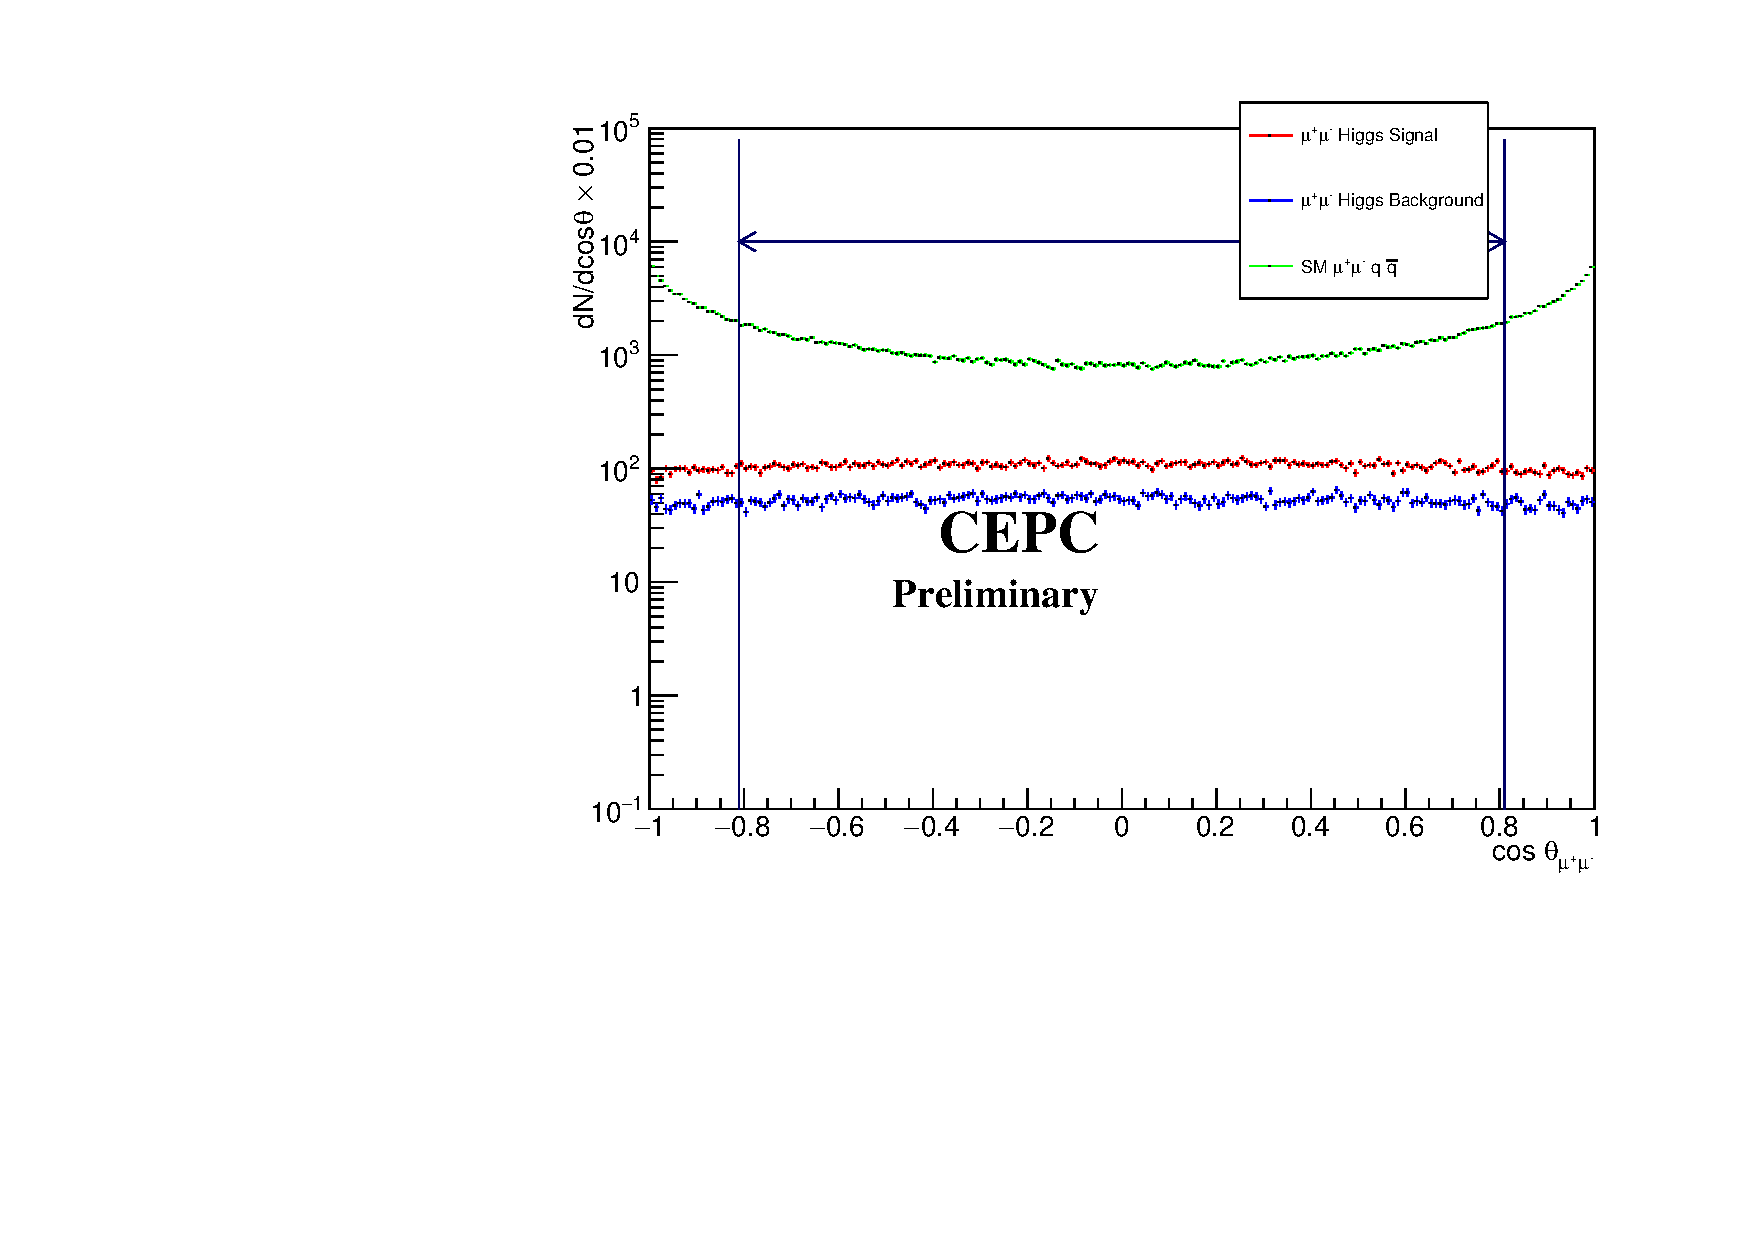
\includegraphics[width=\textwidth]{Analysis/mumuh/ZAngle.pdf}
  \end{minipage}
}
\subfigure[]
{
  \begin{minipage}[b]{0.42\textwidth}
  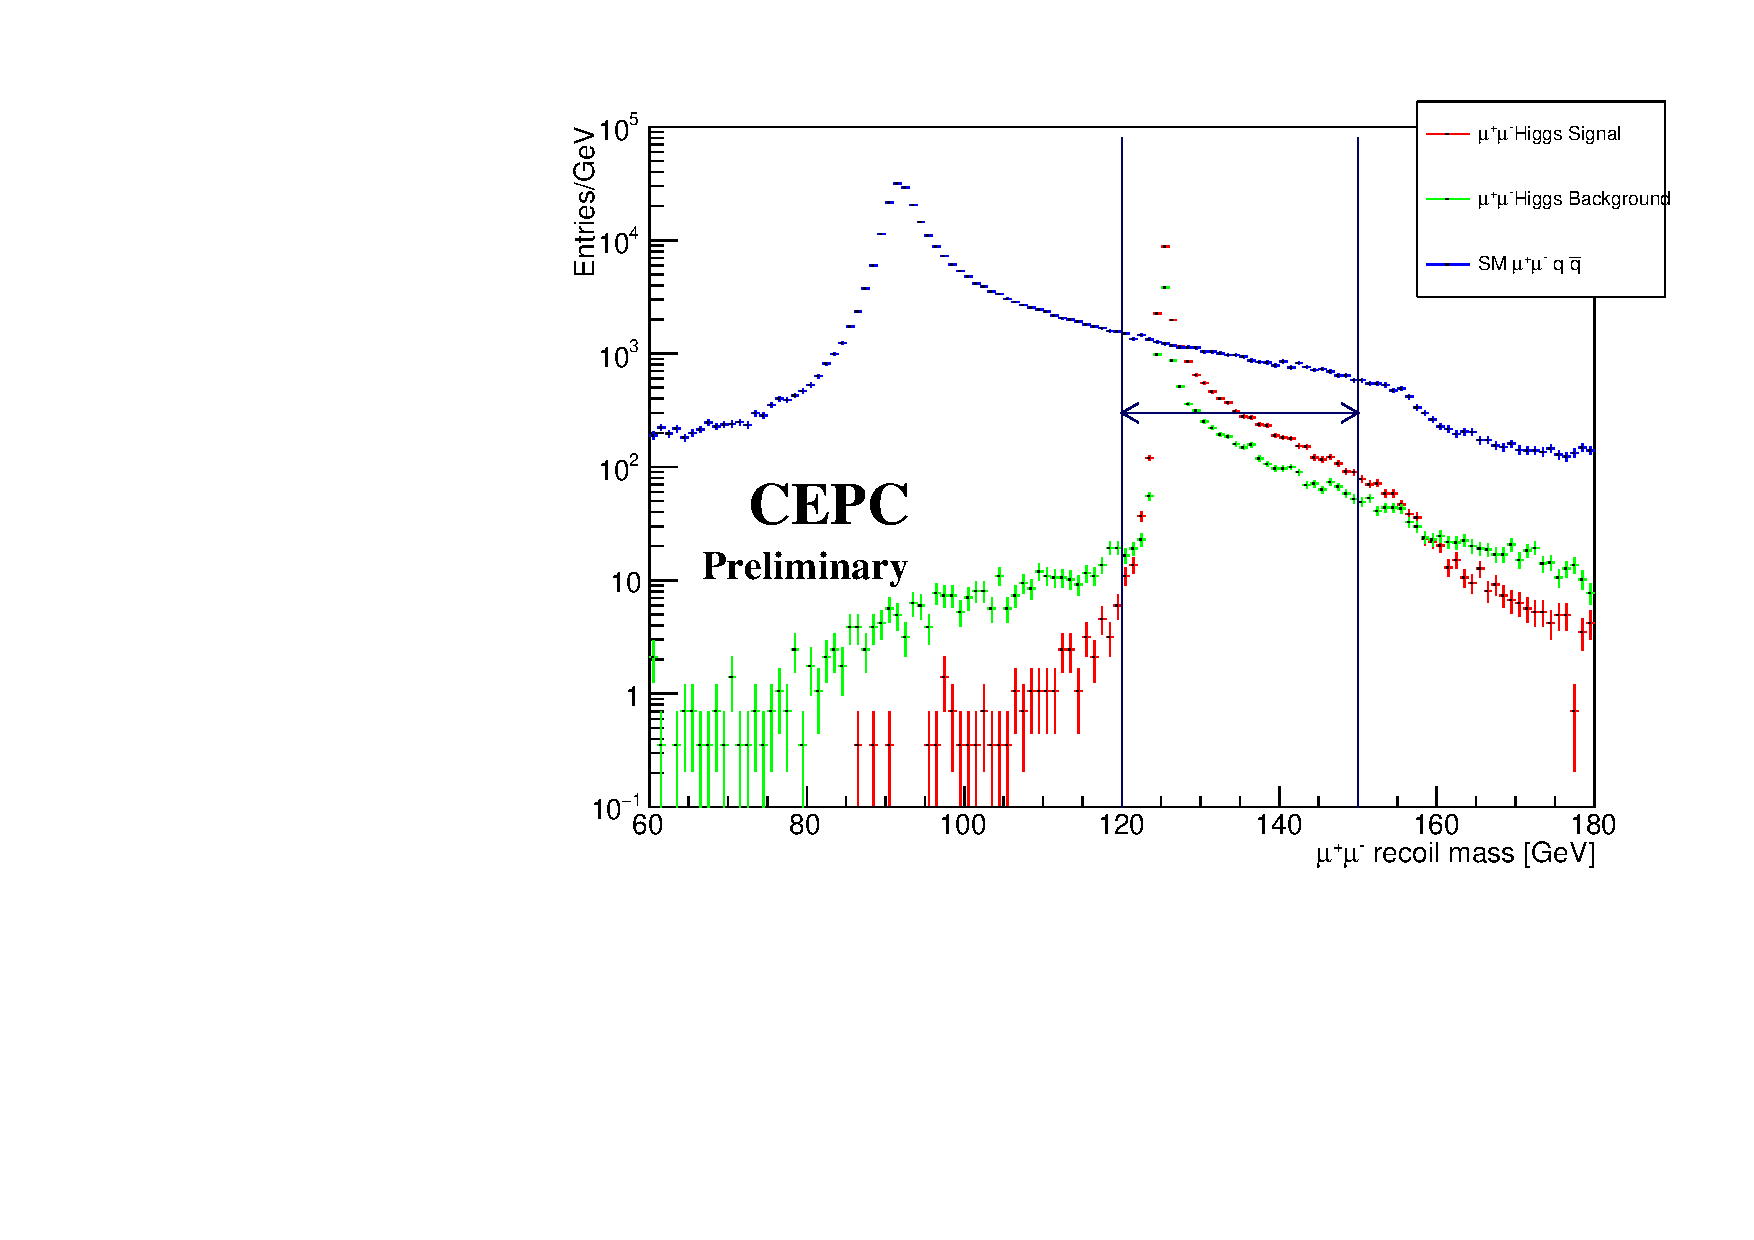
\includegraphics[width=\textwidth]{Analysis/mumuh/mumu_recoil.pdf}
  \end{minipage}
}
\subfigure[]
{ 
   \begin{minipage}[b]{0.42\textwidth}
   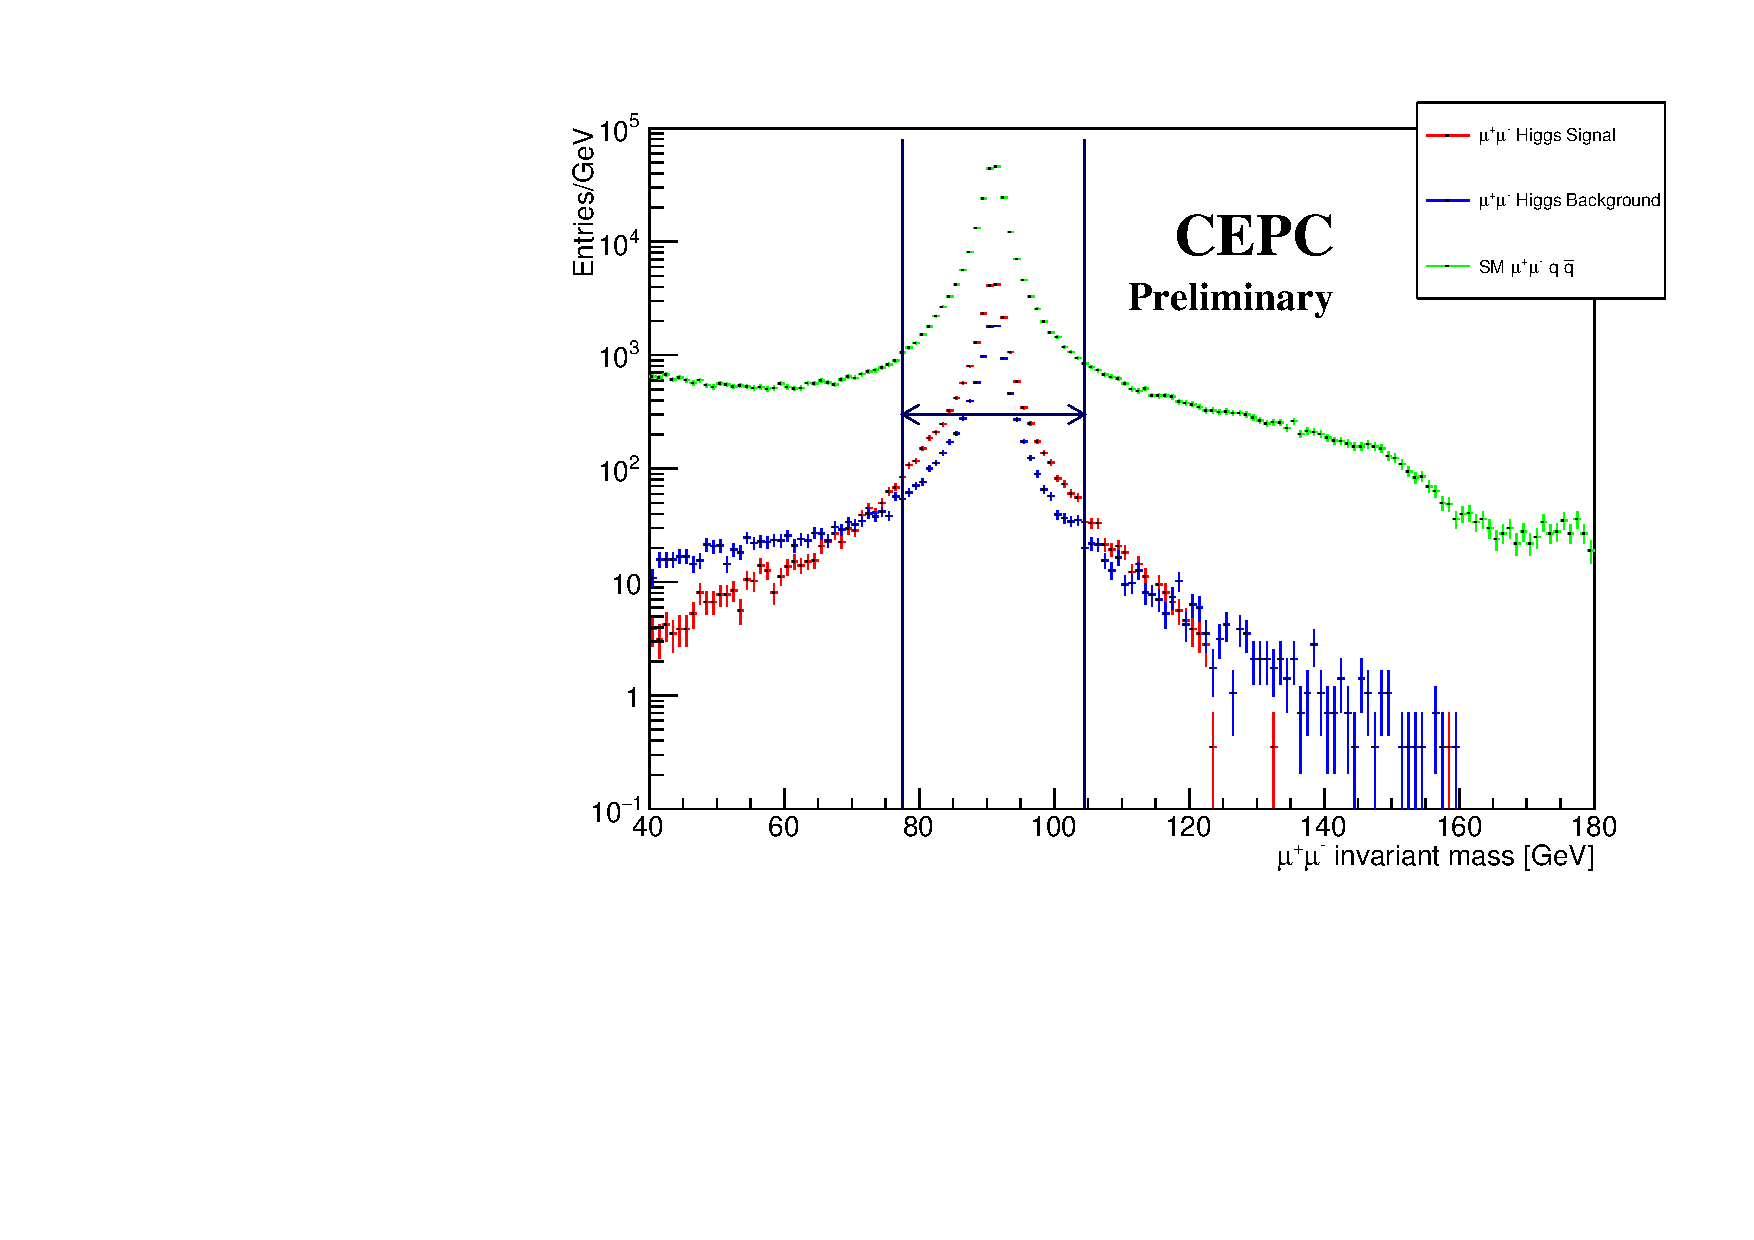
\includegraphics[width=\textwidth]{Analysis/mumuh/mumu_inv.pdf}
   \end{minipage}
}
\subfigure[]
{
    \begin{minipage}[b]{0.42\textwidth}
    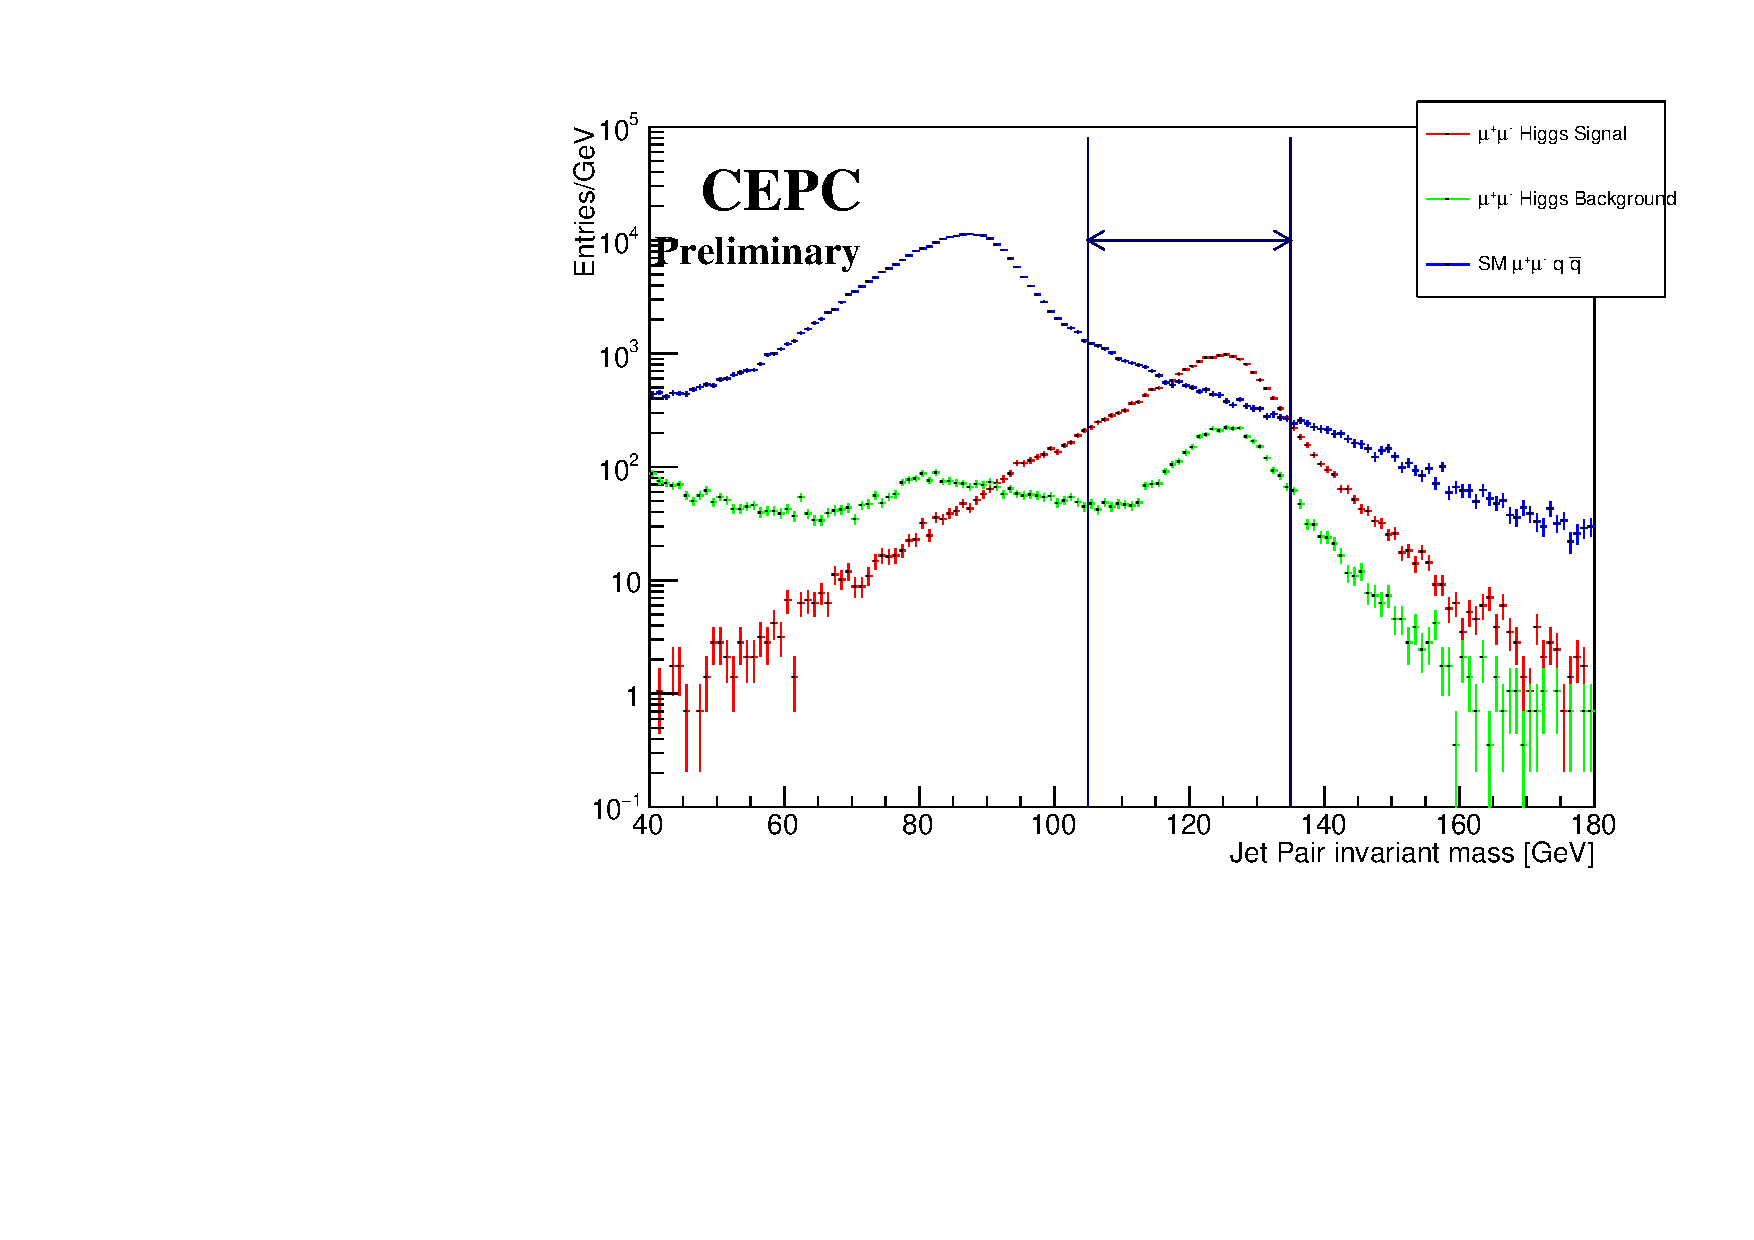
\includegraphics[width=\textwidth]{Analysis/mumuh/JJ_inv.pdf}
    \end{minipage}
}
\caption{Distribution of $\mu^+\mu^-$ system polar angle(top left), $\mu^+\mu^-$ recoil mass(top right), $\mu^+\mu^-$ invariant mass(bottom left) and jet pair invariant mass(bottom right) for signal and dominant backgrounds in $\mmh$ analysis.}
\end{figure}

\begin{table}[!htbp]
\label{tab:mumuh_cut}
\center
\begin{tabular}{c|c|c|c}\hline
%\multicolumn{4}{c|}{$\mmh$} \\ \hline
     Event Yields                          &     Signal   & $\mmh$ background  &  SM $\mu^+\mu^-q\bar{q}$ process \\ \hline
     $\sigma\times$Lumi                    &     24532.3  &      10967.6    &     1051700\\ \hline
       Object Selection                    &     17563.7  &      9203.5                     &    296779.5        \\ \hline
0.85$<\cos\theta_{\mu^+\mu^-}<$0.85        &     18580.8 &      8213.7                         &    193043.4
\\ \hline
120 \GeV$<M_{\mu^+\mu^-recoil}<$150 \GeV   &     17953.2  &      7849.6                       &     19711.2 
\\ \hline 
70 \GeV$<M_{\mu^+\mu^-}<$105               &     17557.1  &      7255.4
&17485.2  \\ \hline
105 \GeV$<M_{JJ}<$135 \GeV                 &     14392.6  &      2927.0 
& 5769.2   \\ \hline
$y_{23}$ \& $y_{34}$ cut                   &     13707.8  &      1575.2 
& 5152.8   \\ \hline 
\end{tabular}
\caption{Event Yields of signal and dominant backgrounds with cuts of $\mmh$ channel, normalized to 5000 \ifb.}
\end{table}

\begin{figure}[!htbp]
\label{fig:kinematic_eeh}
\centering
\subfigure[]
{
  \begin{minipage}[b]{0.42\textwidth}
  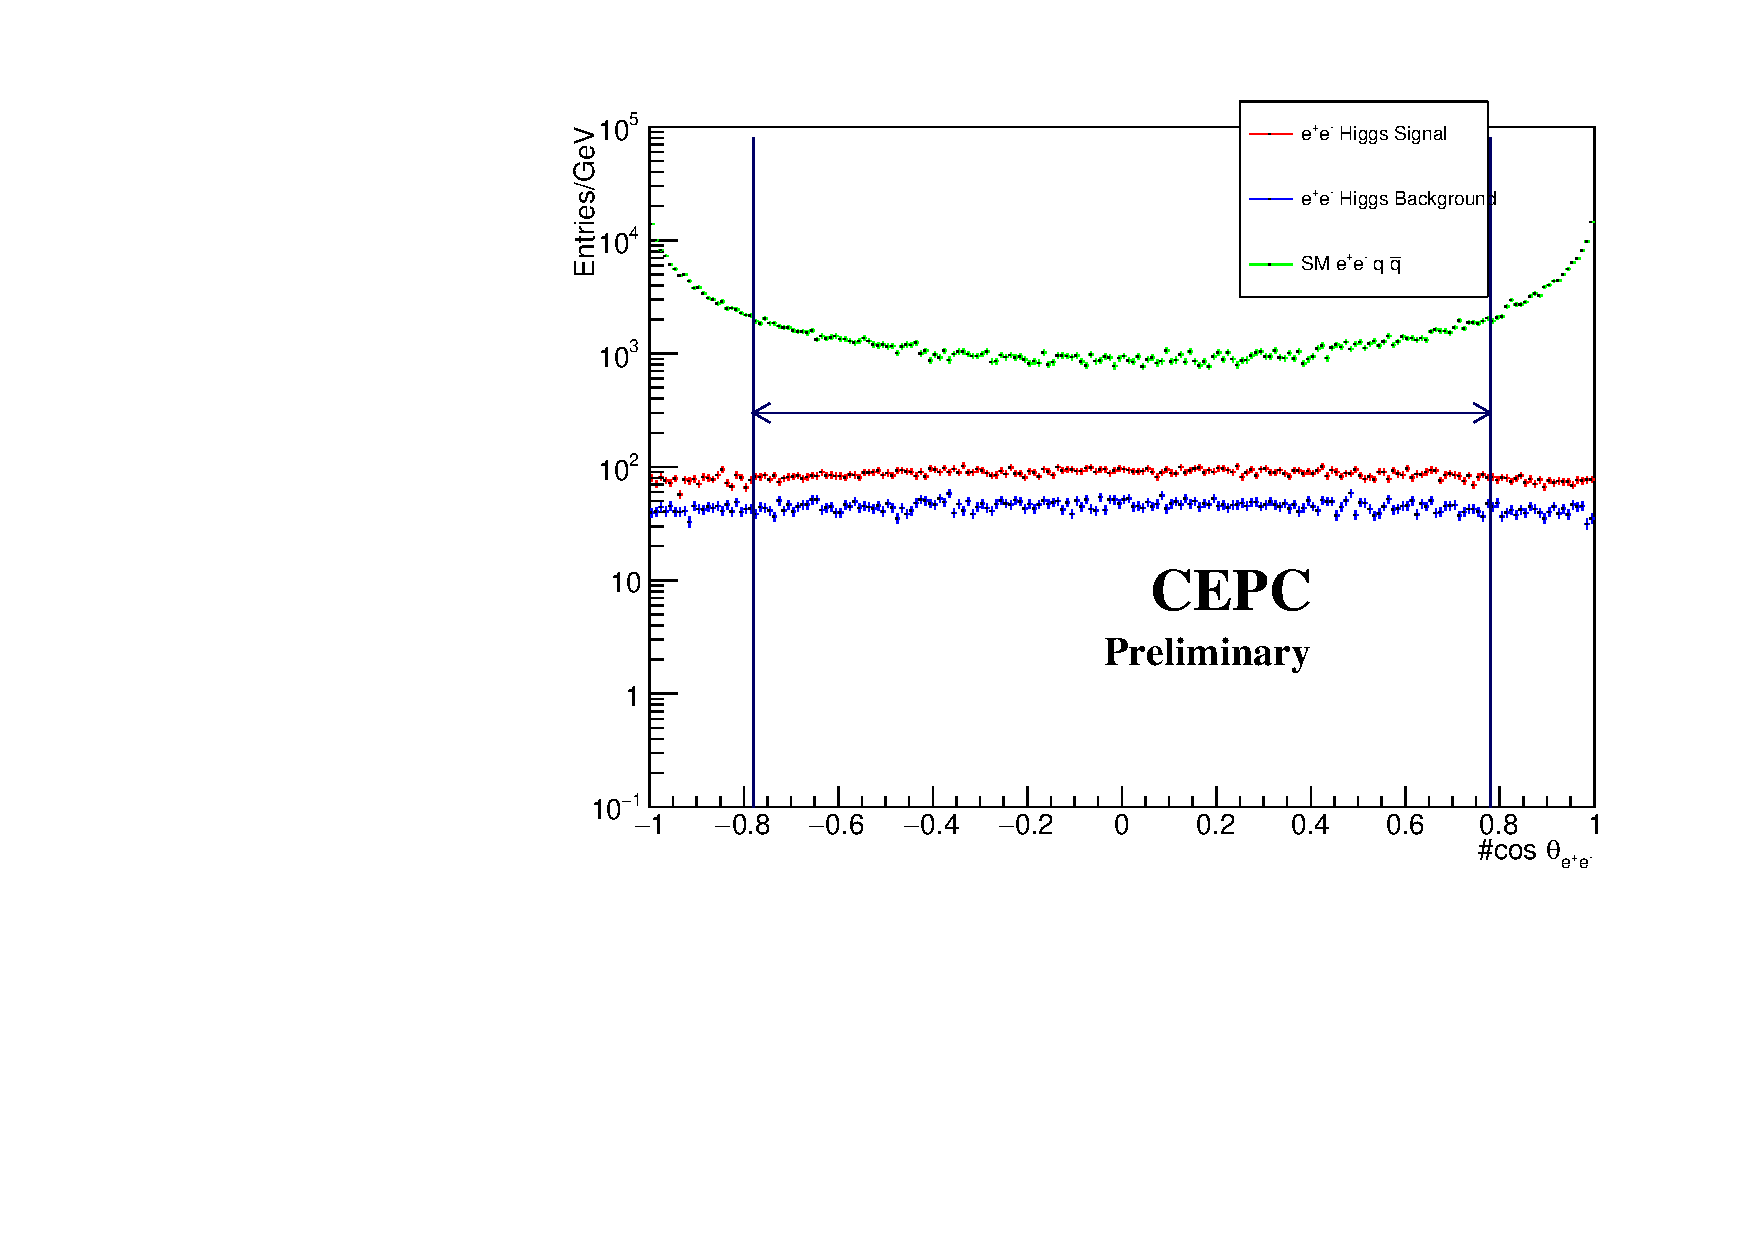
\includegraphics[width=\textwidth]{Analysis/eeh/ZAngle_ee.pdf}
  \end{minipage}
}
\subfigure[]
{
  \begin{minipage}[b]{0.42\textwidth}
  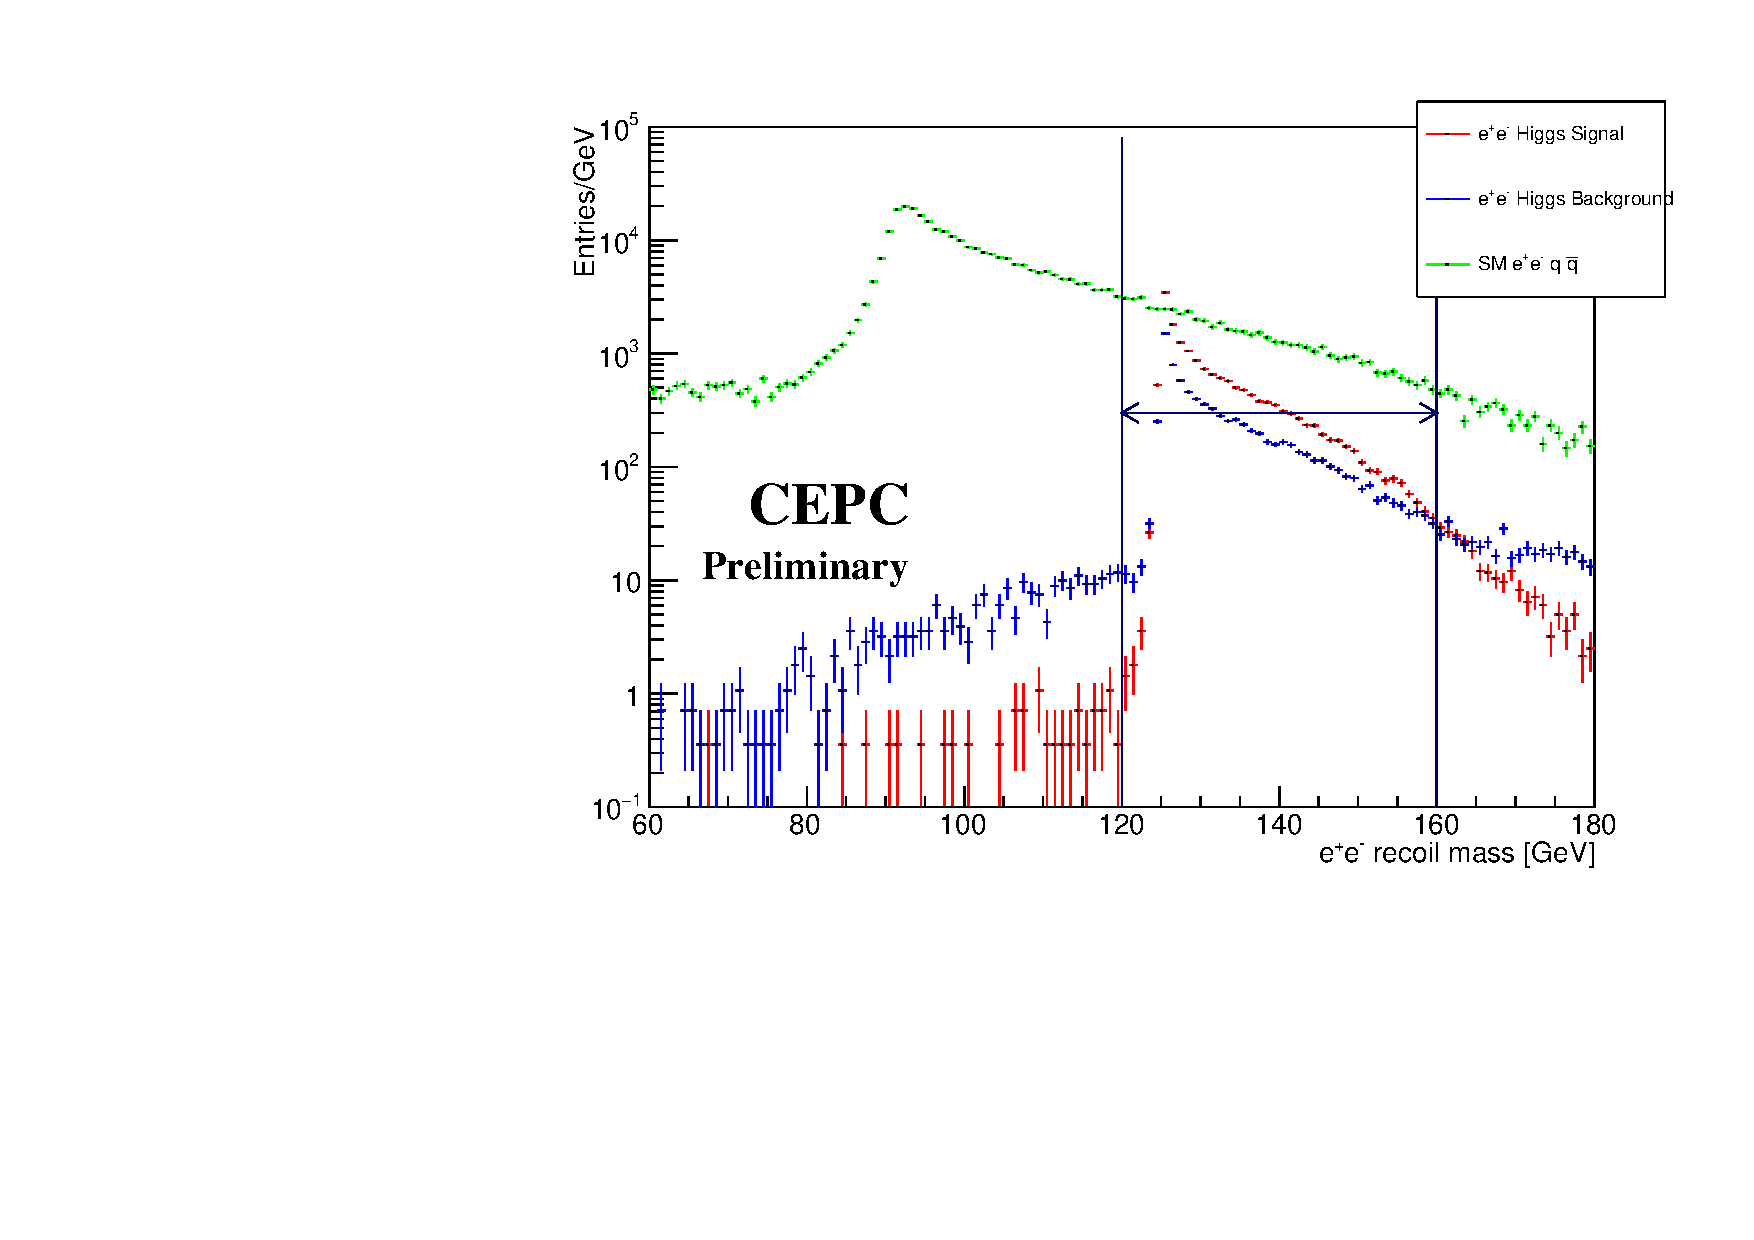
\includegraphics[width=\textwidth]{Analysis/eeh/ee_recoil.pdf}
  \end{minipage}
}
\subfigure[]
{ 
   \begin{minipage}[b]{0.42\textwidth}
   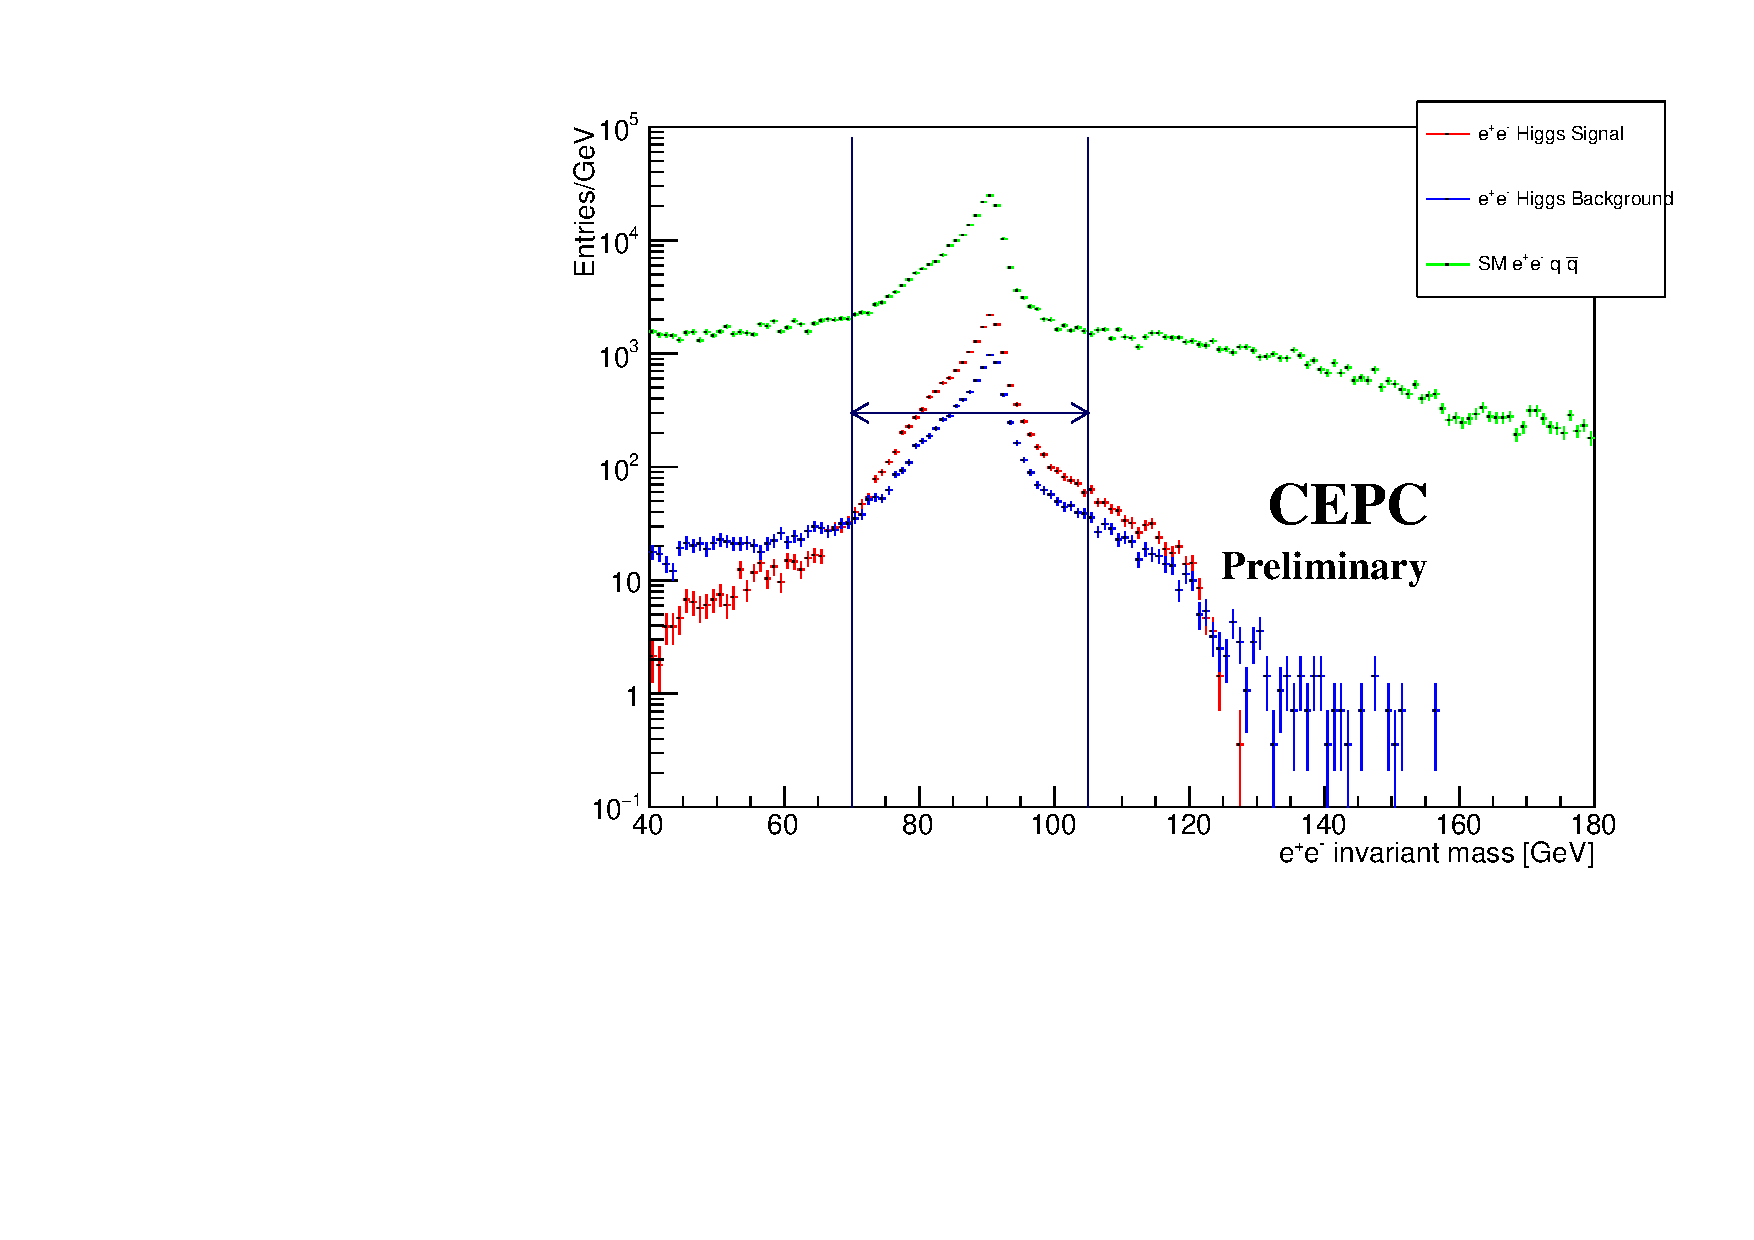
\includegraphics[width=\textwidth]{Analysis/eeh/ee_inv.pdf}
   \end{minipage}
}
\subfigure[]
{
    \begin{minipage}[b]{0.42\textwidth}
    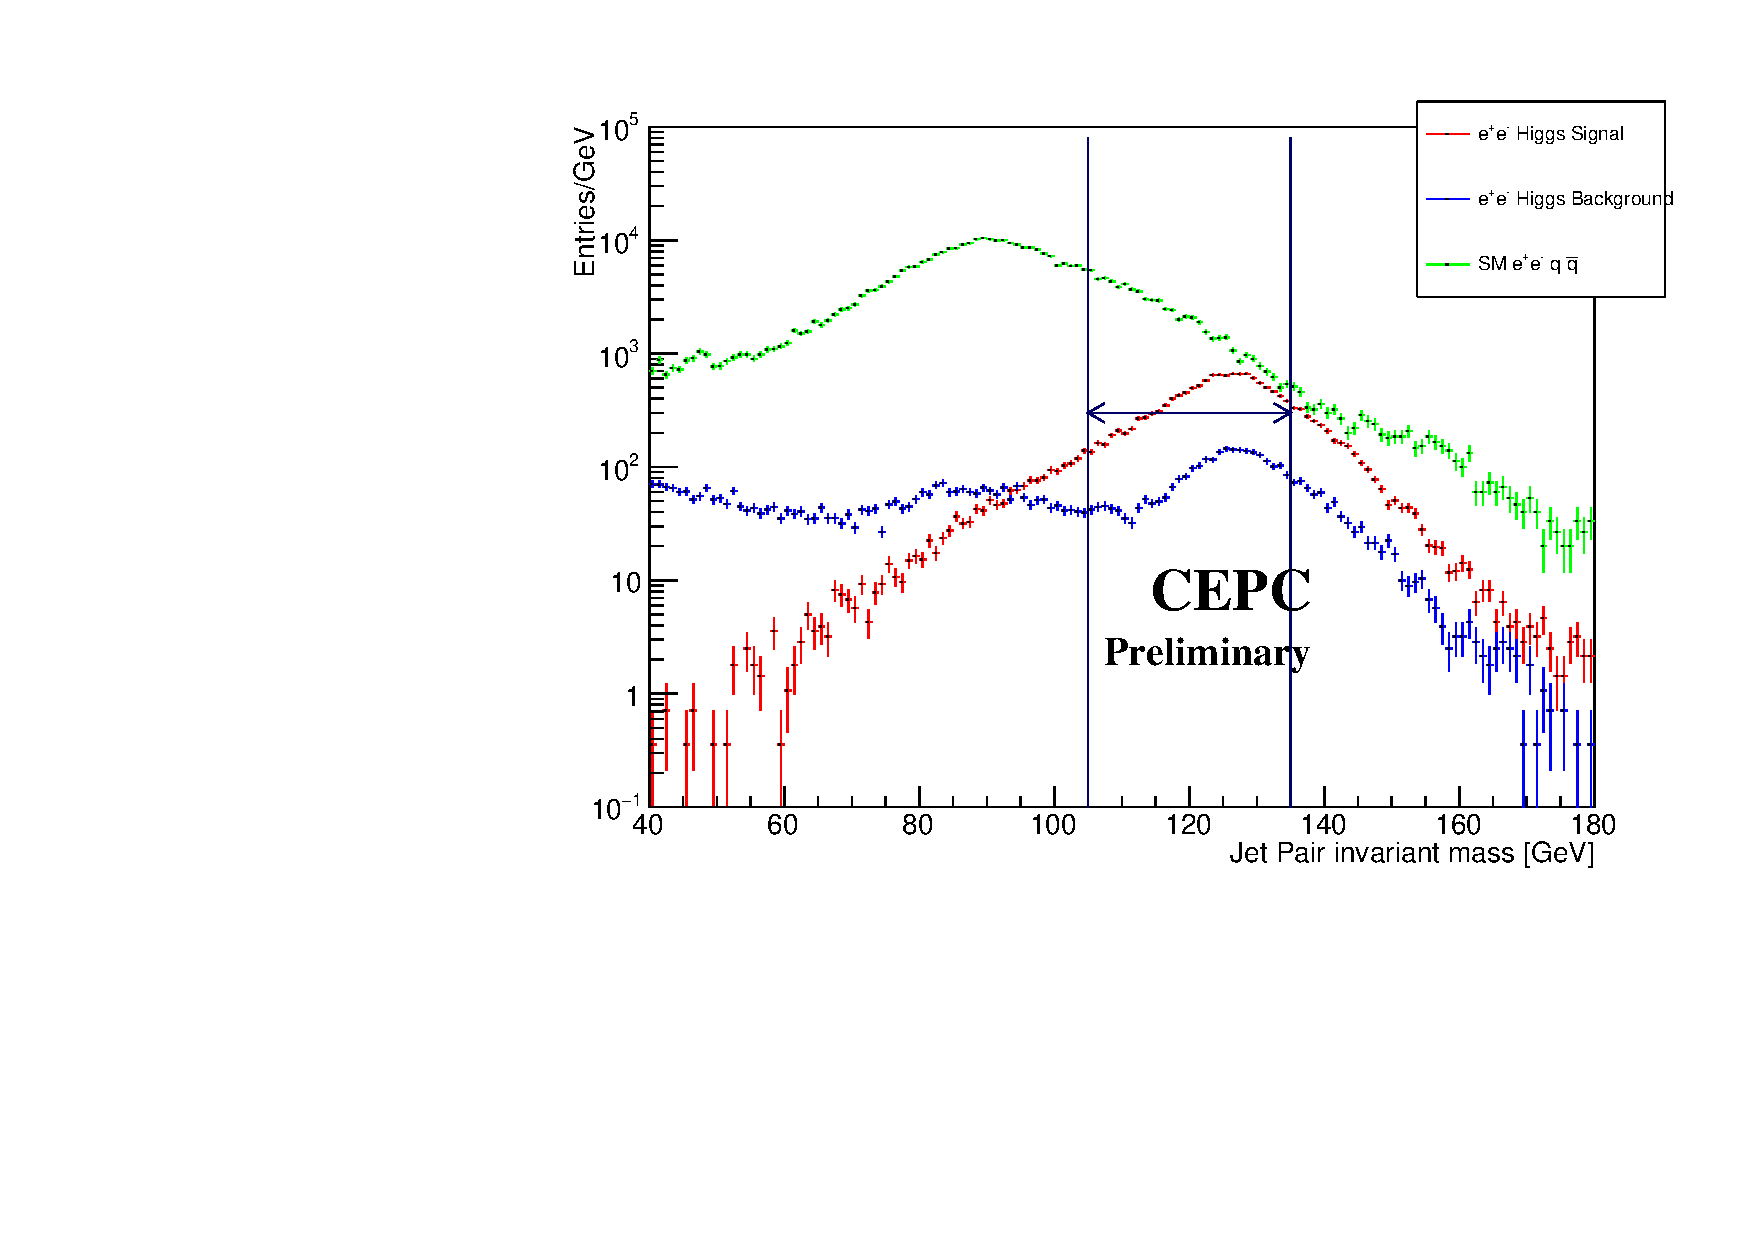
\includegraphics[width=\textwidth]{Analysis/eeh/jj_inv_ee.pdf}
    \end{minipage}
}
\caption{Distribution of $e^+e^-$ system polar angle(top left), $e^+e^-$ recoil mass(top right), $e^+e^-$ invariant mass(bottom left) and jet pair invariant mass(bottom right) for signal and dominant backgrounds in $\eeh$ analysis.}
\end{figure}

\begin{table}[!htbp]
\label{tab:eeh_cut}
\center
\begin{tabular}{c|c|c|c}\hline
%\multicolumn{4}{c|}{$\mmh$} \\ \hline
     Event Yields                          &     Signal   & $\eeh$ background  &  SM $e^+e^-q\bar{q}$ process \\ \hline
     $\sigma\times$Lumi                    &     26438.4  &     11918.6 &   1639129  \\ \hline
       Object Selection                    &     21245.7  &      9192.0                     &    296779.5        \\ \hline
0.78$<\cos\theta_{e^+e^-}<$0.78        &     14002.0  &      7200.8                         &    372942.9
\\ \hline
120 \GeV$<M_{e^+e^-recoil}<$160 \GeV   &     13773.9  &      6581.0                         &    167607.0 
\\ \hline 
70 \GeV$<M_{e^+e^-}<$105               &     13143.0  &      6051.4
&27027.4  \\ \hline
105 \GeV$<M_{JJ}<$135 \GeV                 &     9637.7   &      1935.3 
& 6941.2   \\ \hline
$y_{23}$ \& $y_{34}$ cut                    &    9148.4  &       1101.9 
& 6081.4   \\ \hline 
\end{tabular}
\caption{Event Yields of signal and dominant backgrounds with cuts of $\eeh$ channel, normalized to 5000 \ifb.}
\end{table}
%\clearpage

\subsection{\nnh Event Selection}
The \nnh channel includes $ZH$ production followed by invisible $Z-$decay, or $t-$channel $W-$fusion process. 
The dominant backgrounds are quark pair production and gauge boson pair production, followed by hadronic and invisible decay of each boson. 
The observable particles in the signal form two energetic jets, initiated from two quarks of higgs decay. 
Thus isolation leptons are rejected, and a minimum number of PFOs are required the quark pair. 
The signal events are featured in the kinematic distribution of invisible section.  
The visible energy of the signal events are significantly lower than reducible SM backgrounds like semi-leptonic $WW$ events. 
The visible transverse momentum are required to larger than 19 \GeV to reject \qq events, which tend to have low visible tranverse momentum due to 
high fraction of radiation return events.
The invariant mass of the jets characterize the higgs production which is obverse discriminator against the non-higgs production SM events
\footnote{The peak of in signal region of \qq events is due to radiation events.}.
The angle between two jets and $y$-th values are also useful to distinguish signal events from SM backgrounds.  
Meanwhile the recoil system of these two jets, which is not directly observable, has the charaterstic of the $Z$ boson associate with higgs in final states. The distribution of the above varibles and cut value can be found in figure \ref{fig:kinematic_nnh} and \ref{fig:yth_nnh} for signal and background events. \par

The Boost decision tree \cite{BDT} method is implemented to the survived events from cut chain. The variables used 
in BDT are mentioned aboved: visible energy,  transverse momentum, $y-th$ value, jet pair recoil and invariant mass. 
The events yields of signal and background in cutflow and BDT selection can be found in table \ref{tab:nnh_cut}. \par


\begin{figure}[!htbp]
\label{fig:kinematic_nnh}
\centering
\subfigure[]
{
  \begin{minipage}[b]{0.31\textwidth}
  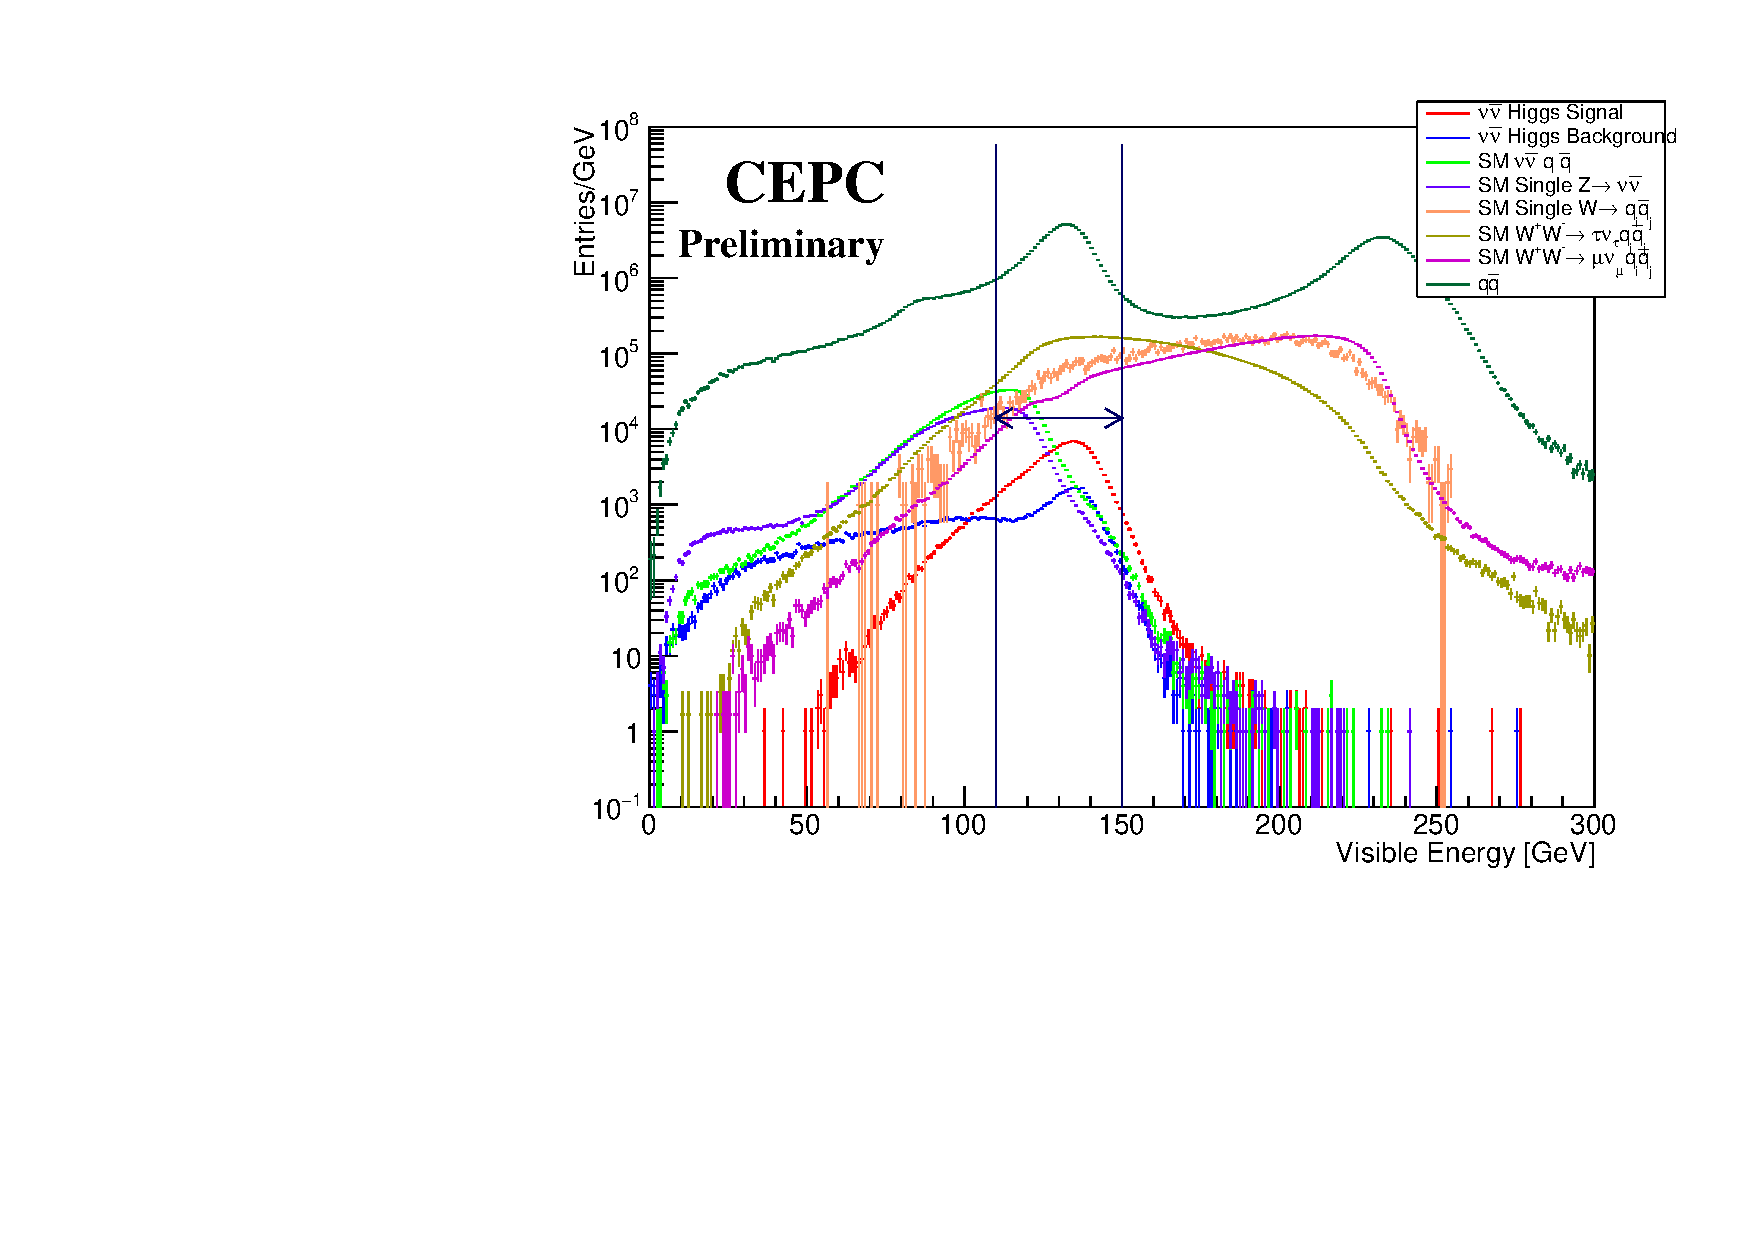
\includegraphics[width=\textwidth]{Analysis/nnh/Etot.pdf}
  \end{minipage}
}
\subfigure[]
{
  \begin{minipage}[b]{0.31\textwidth}
  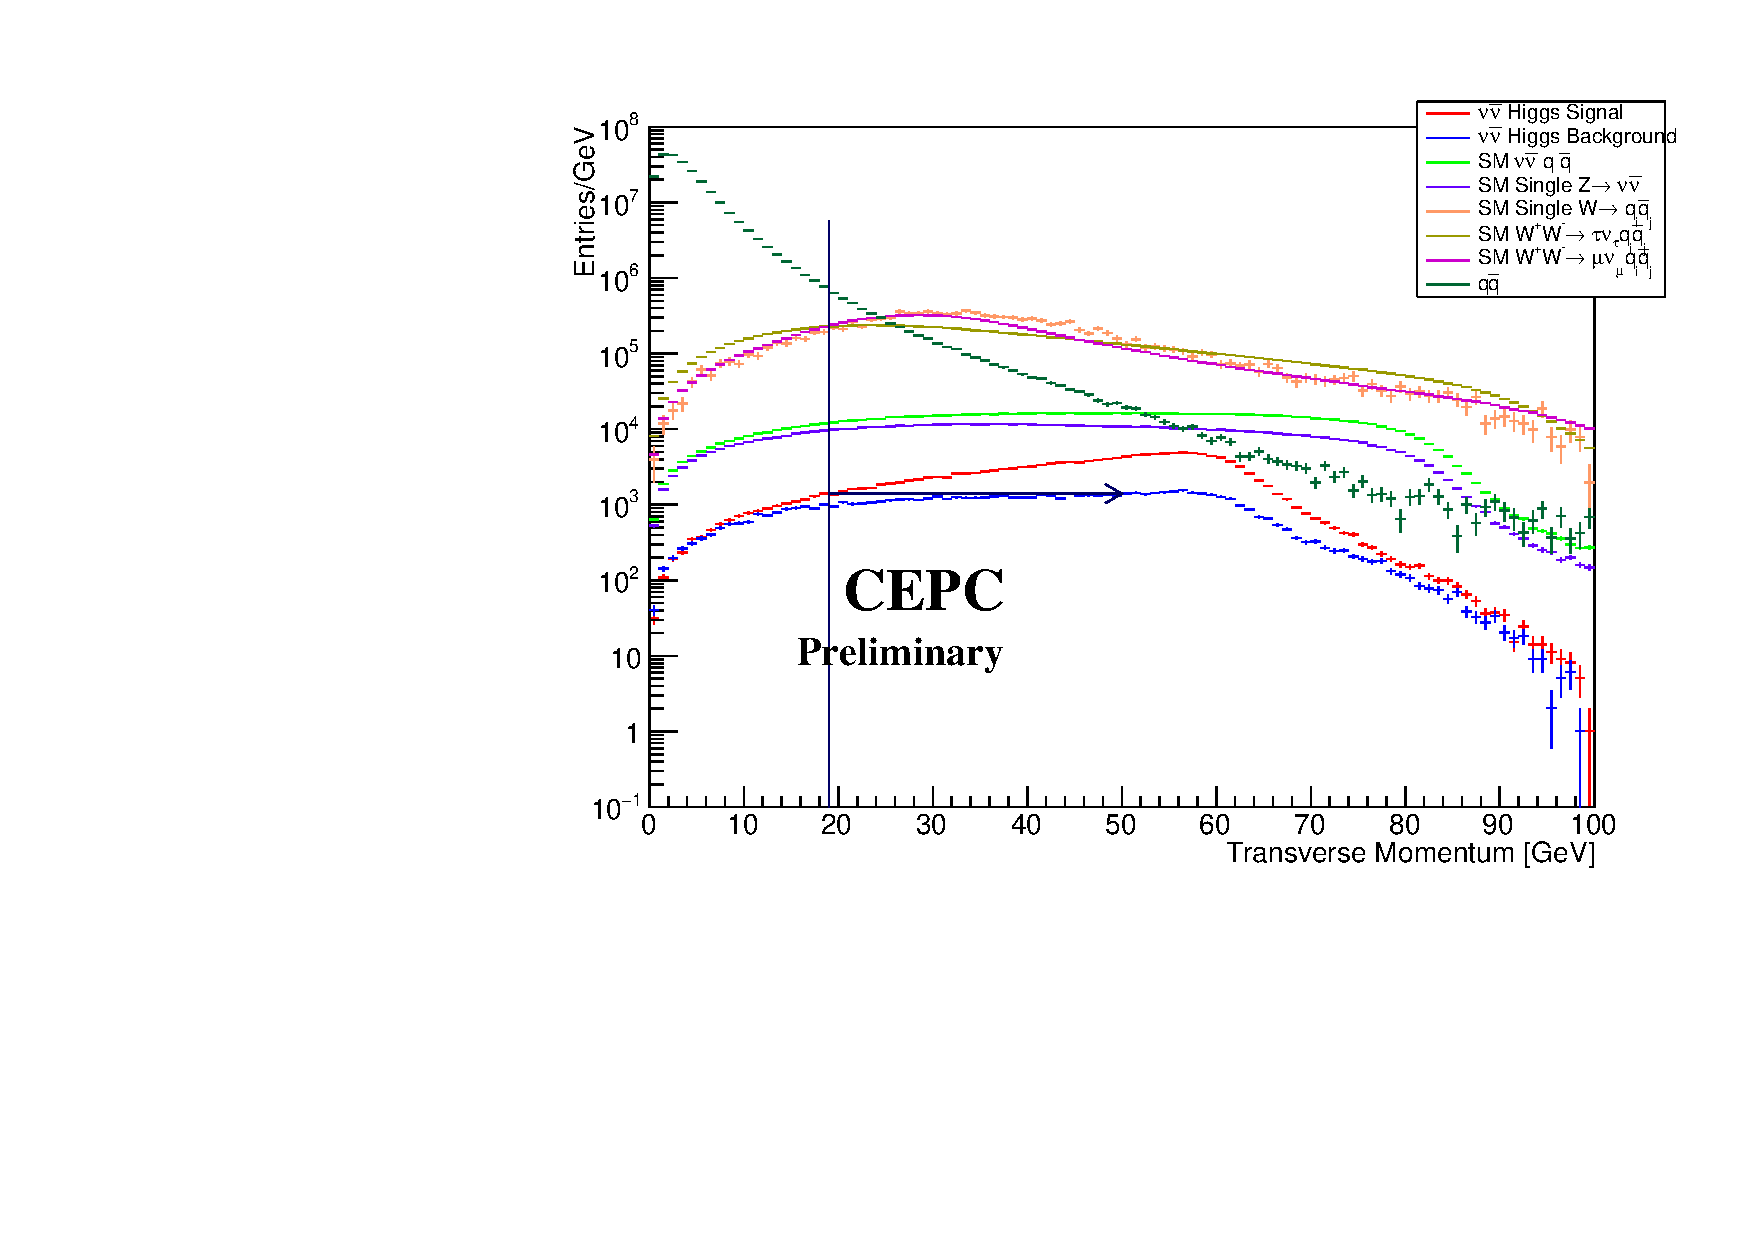
\includegraphics[width=\textwidth]{Analysis/nnh/pT.pdf}
  \end{minipage}
}
\subfigure[]
{
  \begin{minipage}[b]{0.31\textwidth}
  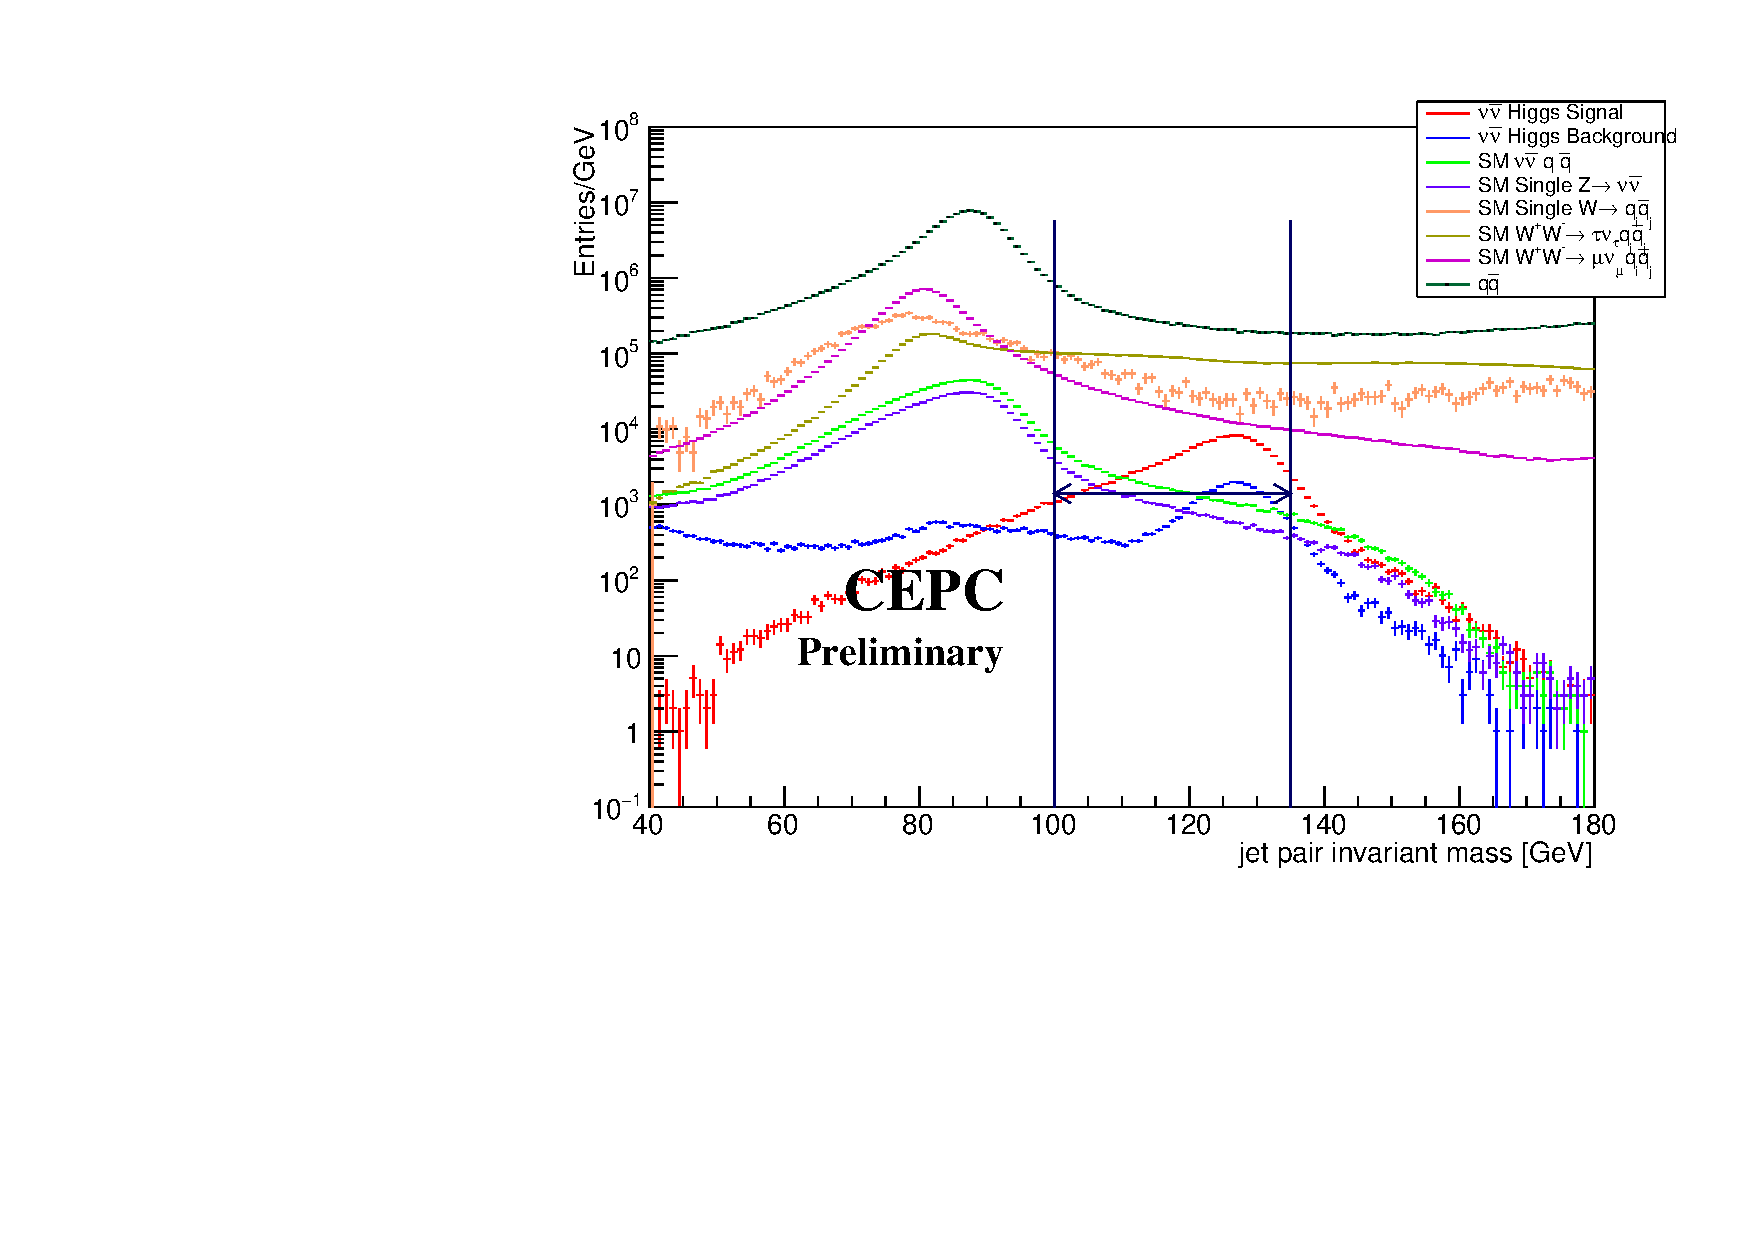
\includegraphics[width=\textwidth]{Analysis/nnh/jj_inv.pdf}
  \end{minipage}
}
\subfigure[]
{ 
   \begin{minipage}[b]{0.31\textwidth}
   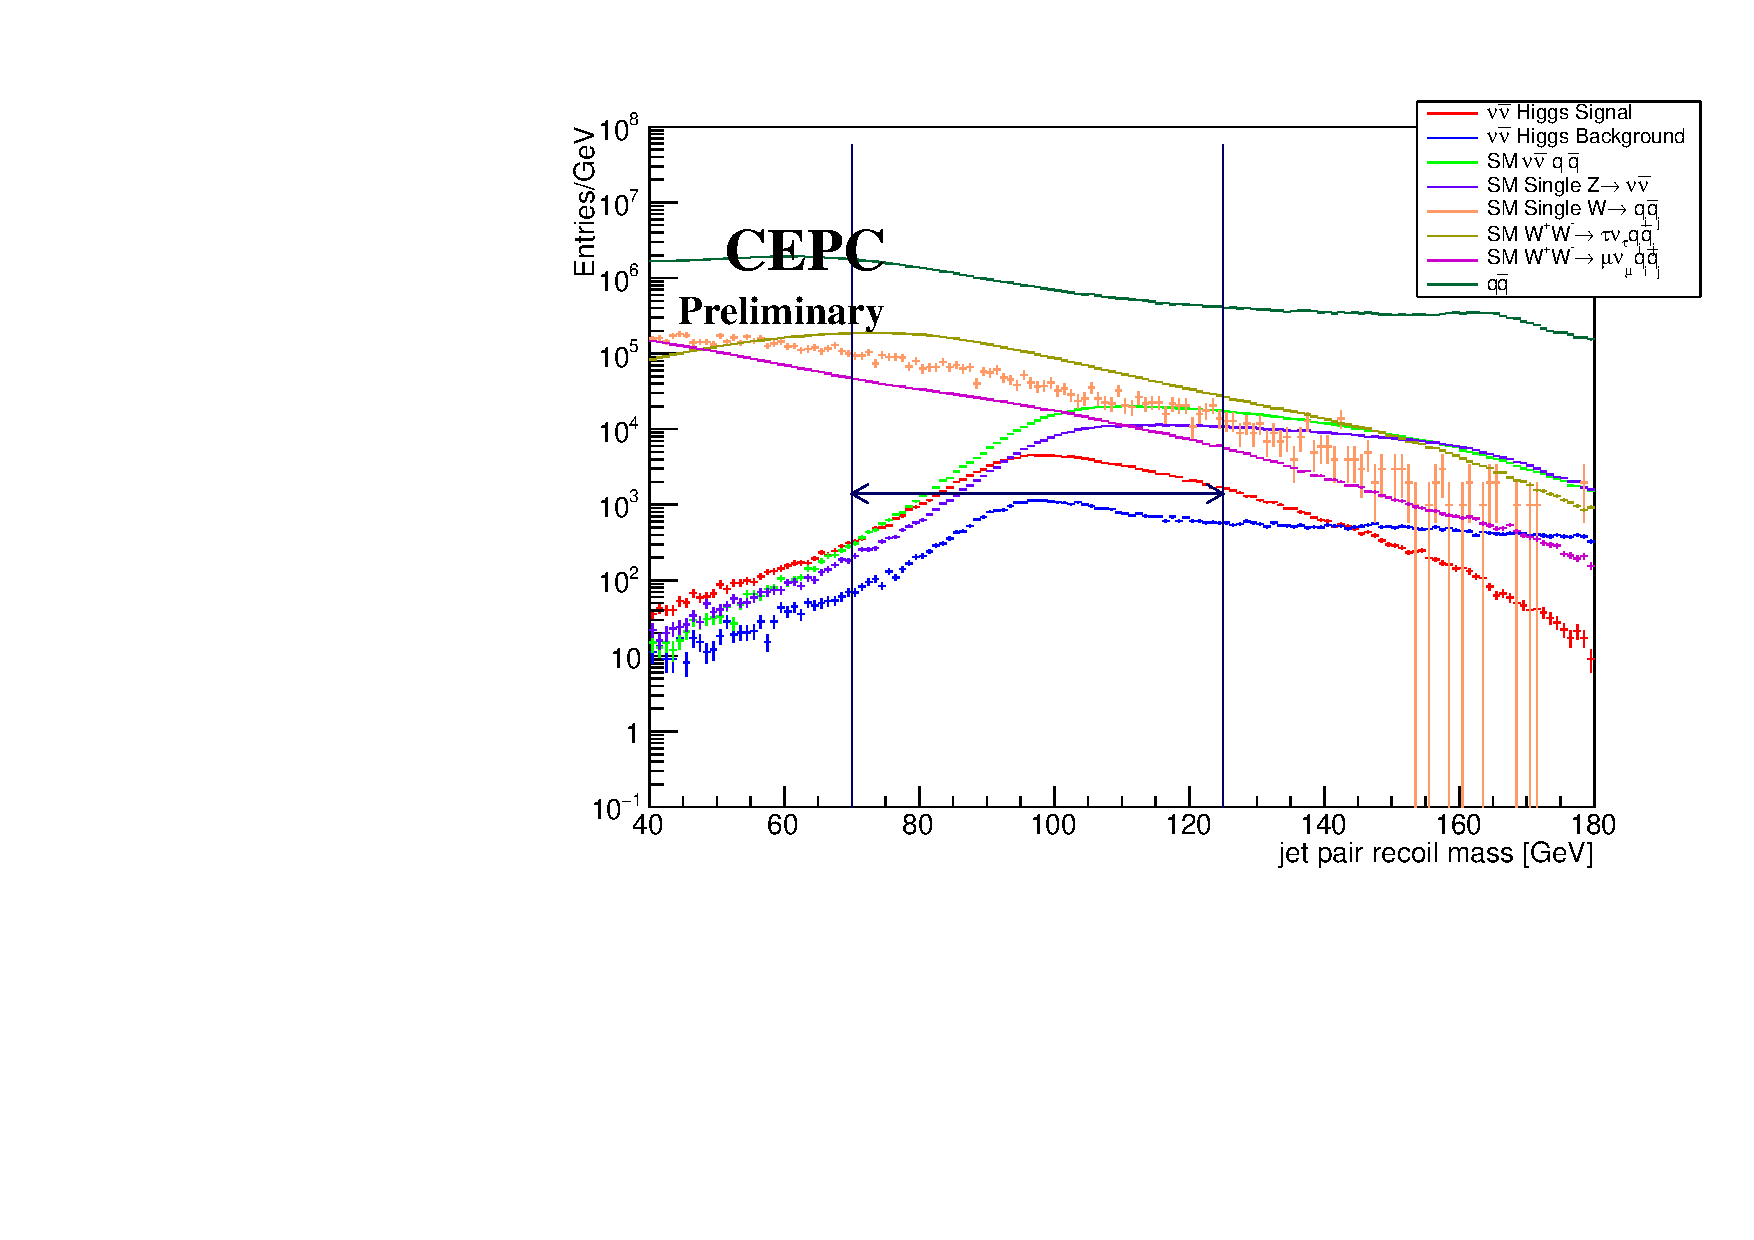
\includegraphics[width=\textwidth]{Analysis/nnh/jj_recoil.pdf}
   \end{minipage}
}
\subfigure[]
{
    \begin{minipage}[b]{0.31\textwidth}
    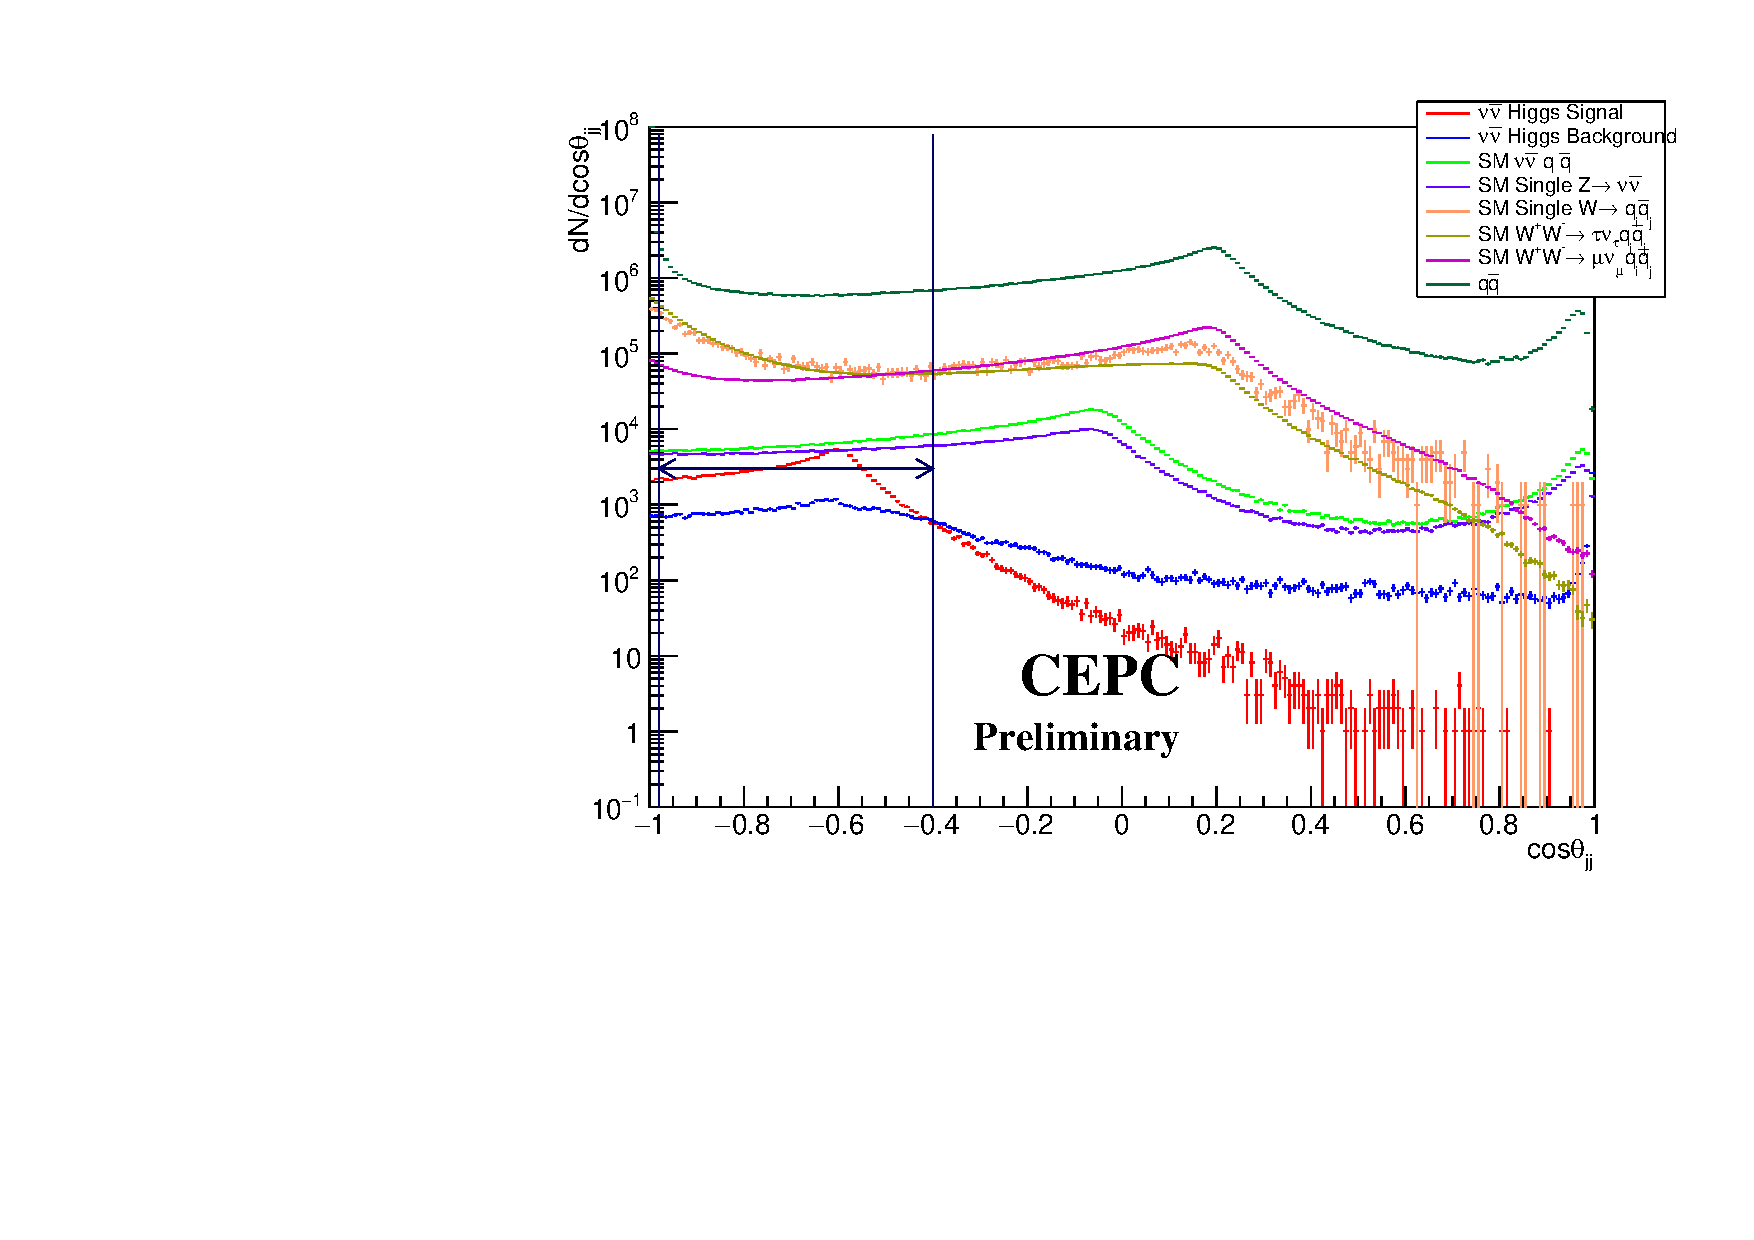
\includegraphics[width=\textwidth]{Analysis/nnh/costheta.pdf}
    \end{minipage}
}
\caption{Visible energy(top left), visible transverse momentum(top middle), jet pair system invariant mass(top right), jet system recoil mass(bottom left) and jet pair system polar angluar(bottom right) distribution in \nnh analysis.}
\end{figure}

\begin{figure}[!htpb]
\label{fig:yth_nnh}
\centering
\subfigure[]
{
  \begin{minipage}[b]{0.31\textwidth}
  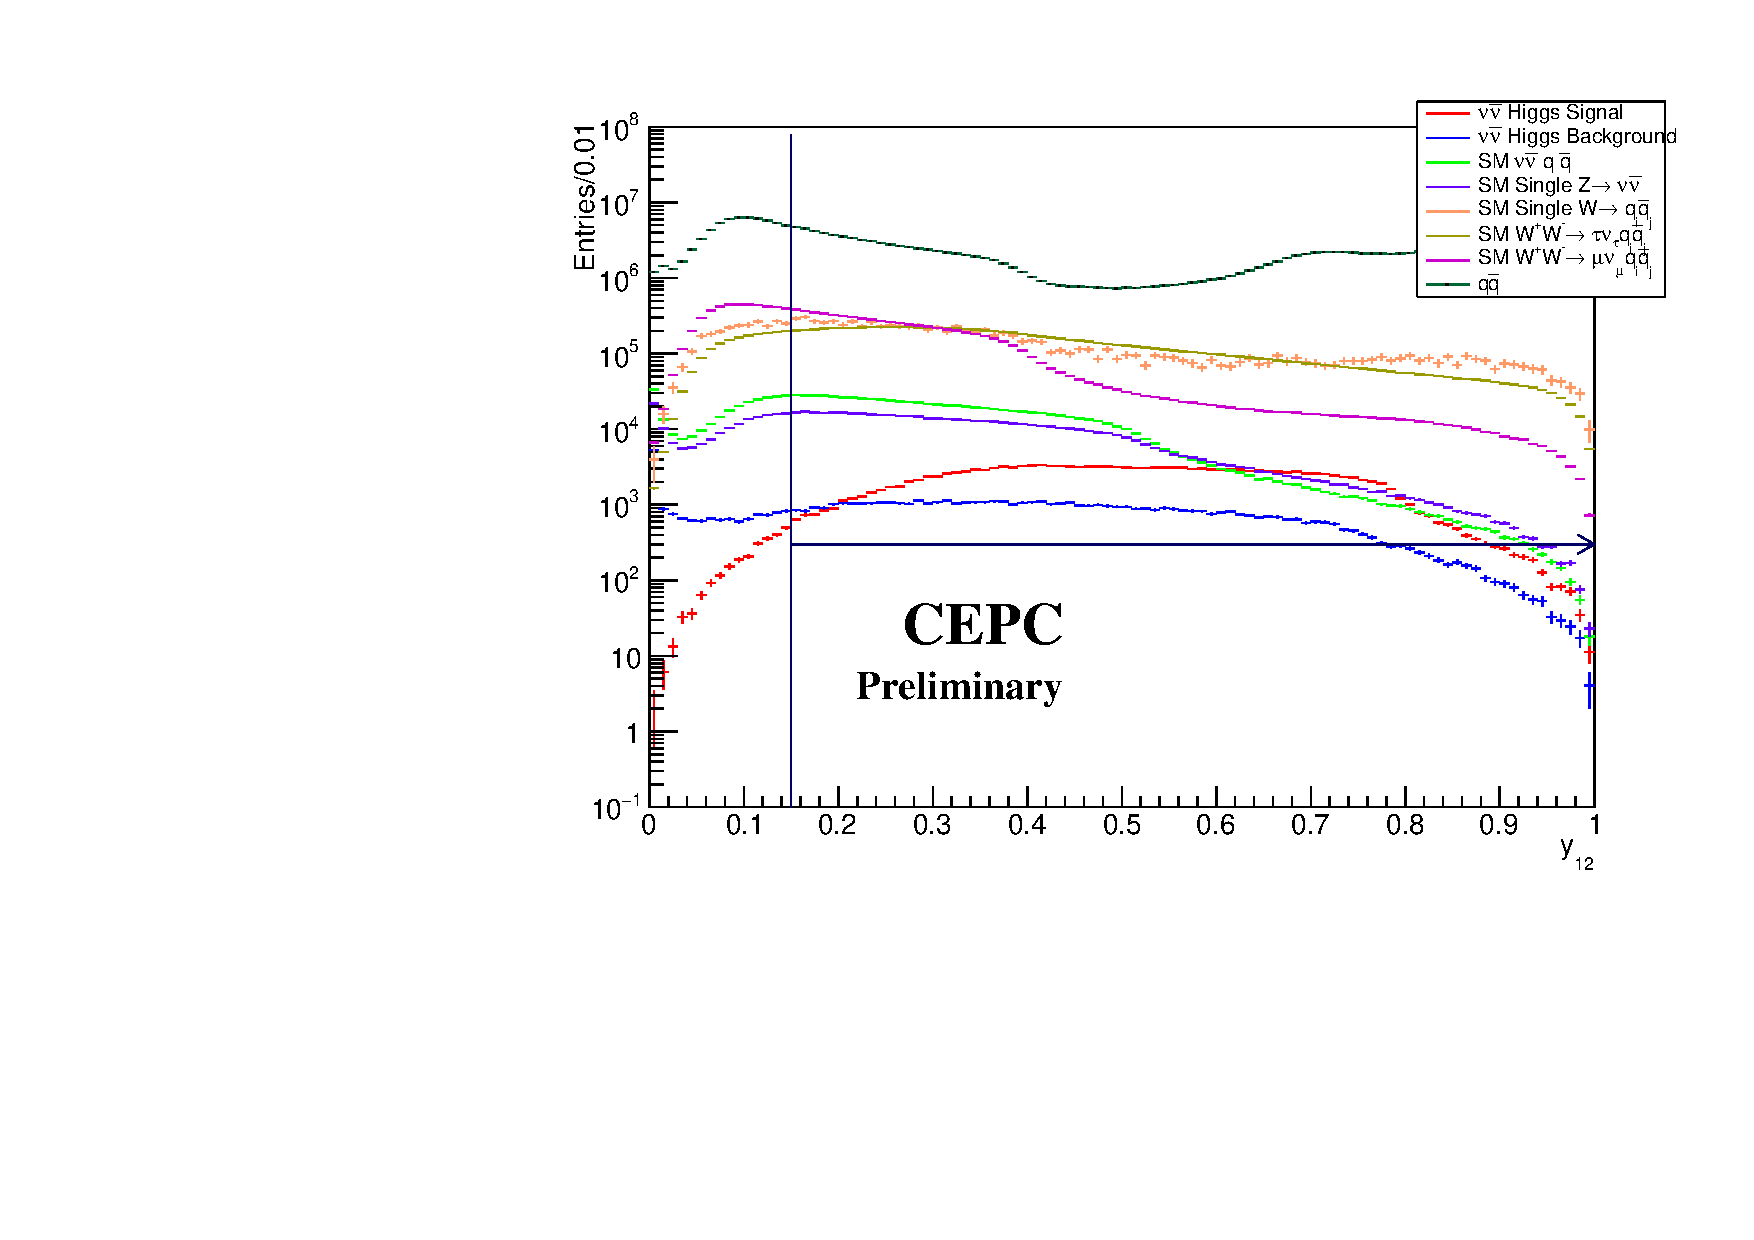
\includegraphics[width=\textwidth]{Analysis/nnh/y12.pdf}
  \end{minipage}   
}
\subfigure[]
{
  \begin{minipage}[b]{0.31\textwidth}
  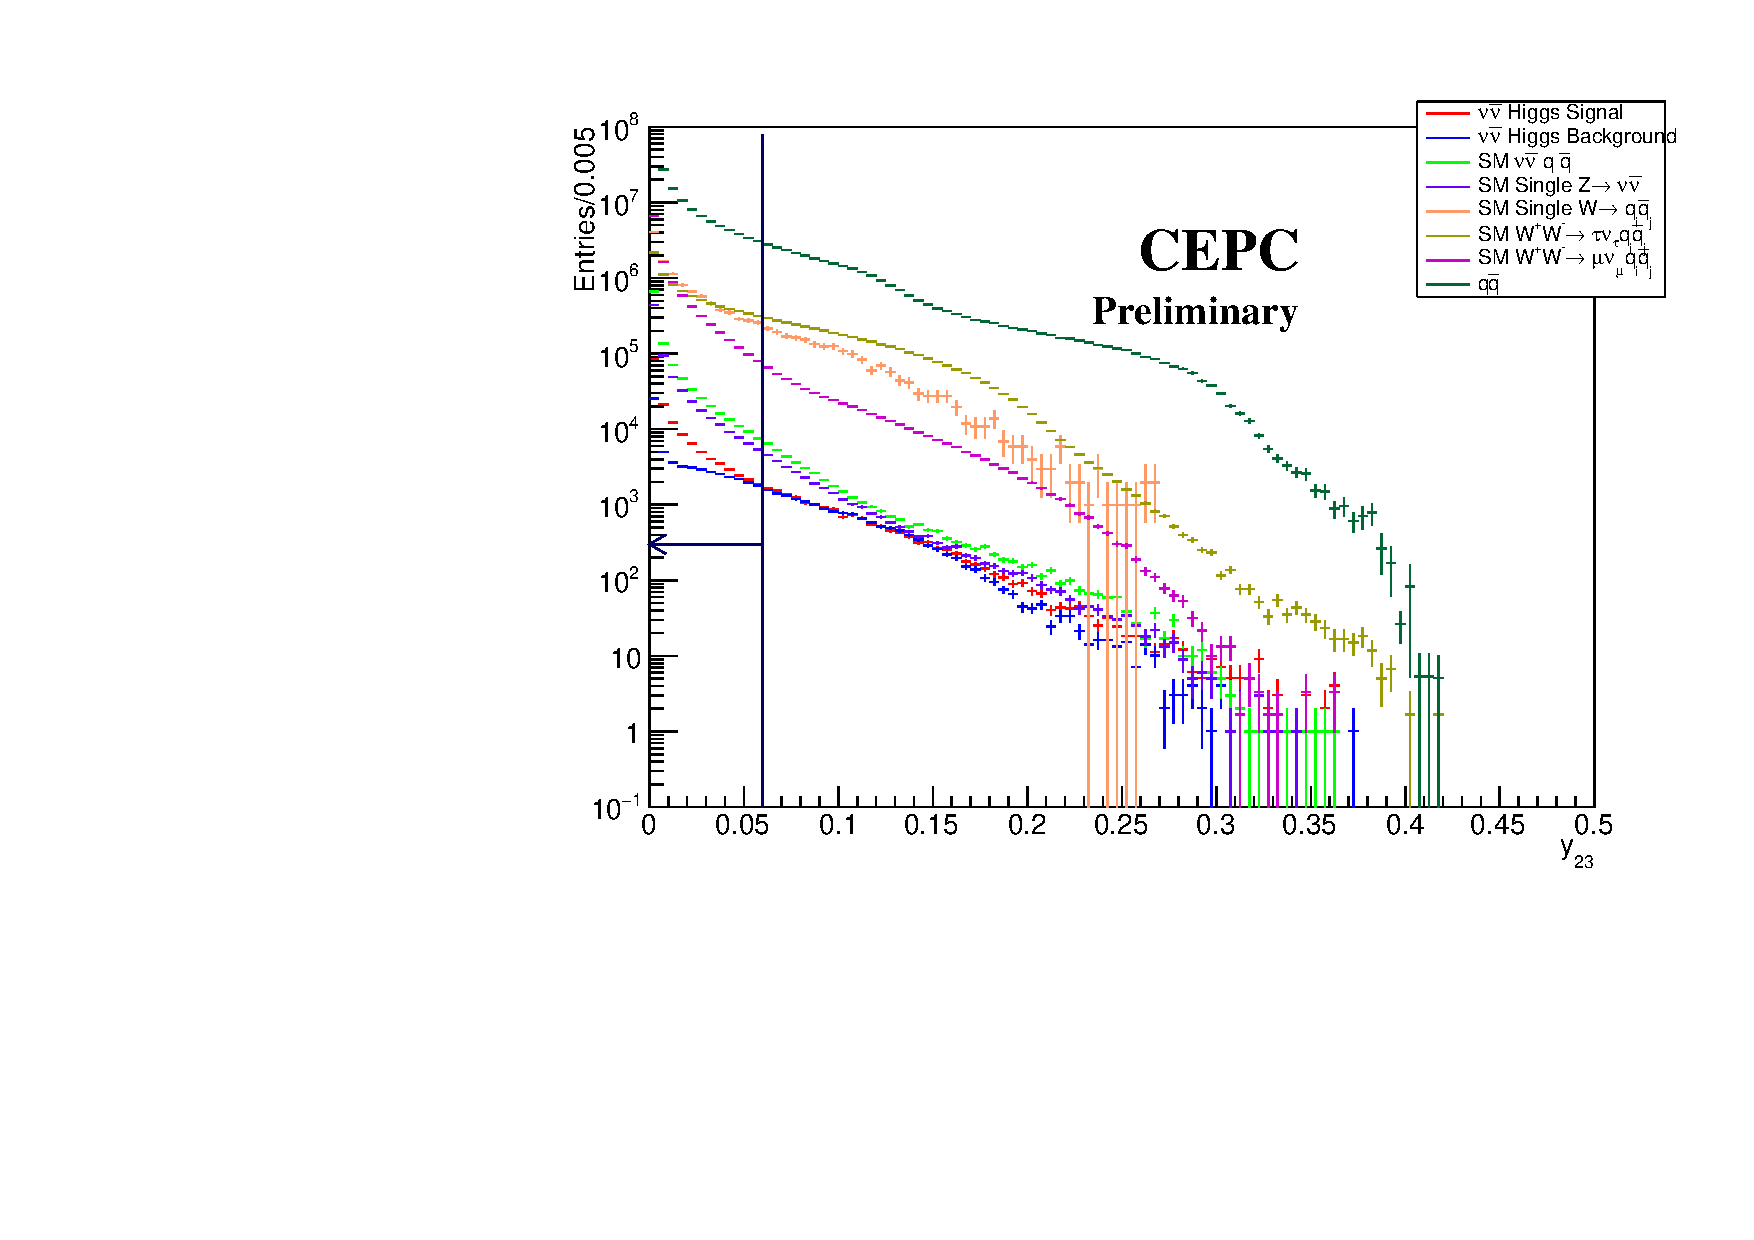
\includegraphics[width=\textwidth]{Analysis/nnh/y23.pdf}
  \end{minipage}
}
\subfigure[]
{
  \begin{minipage}[b]{0.31\textwidth}
  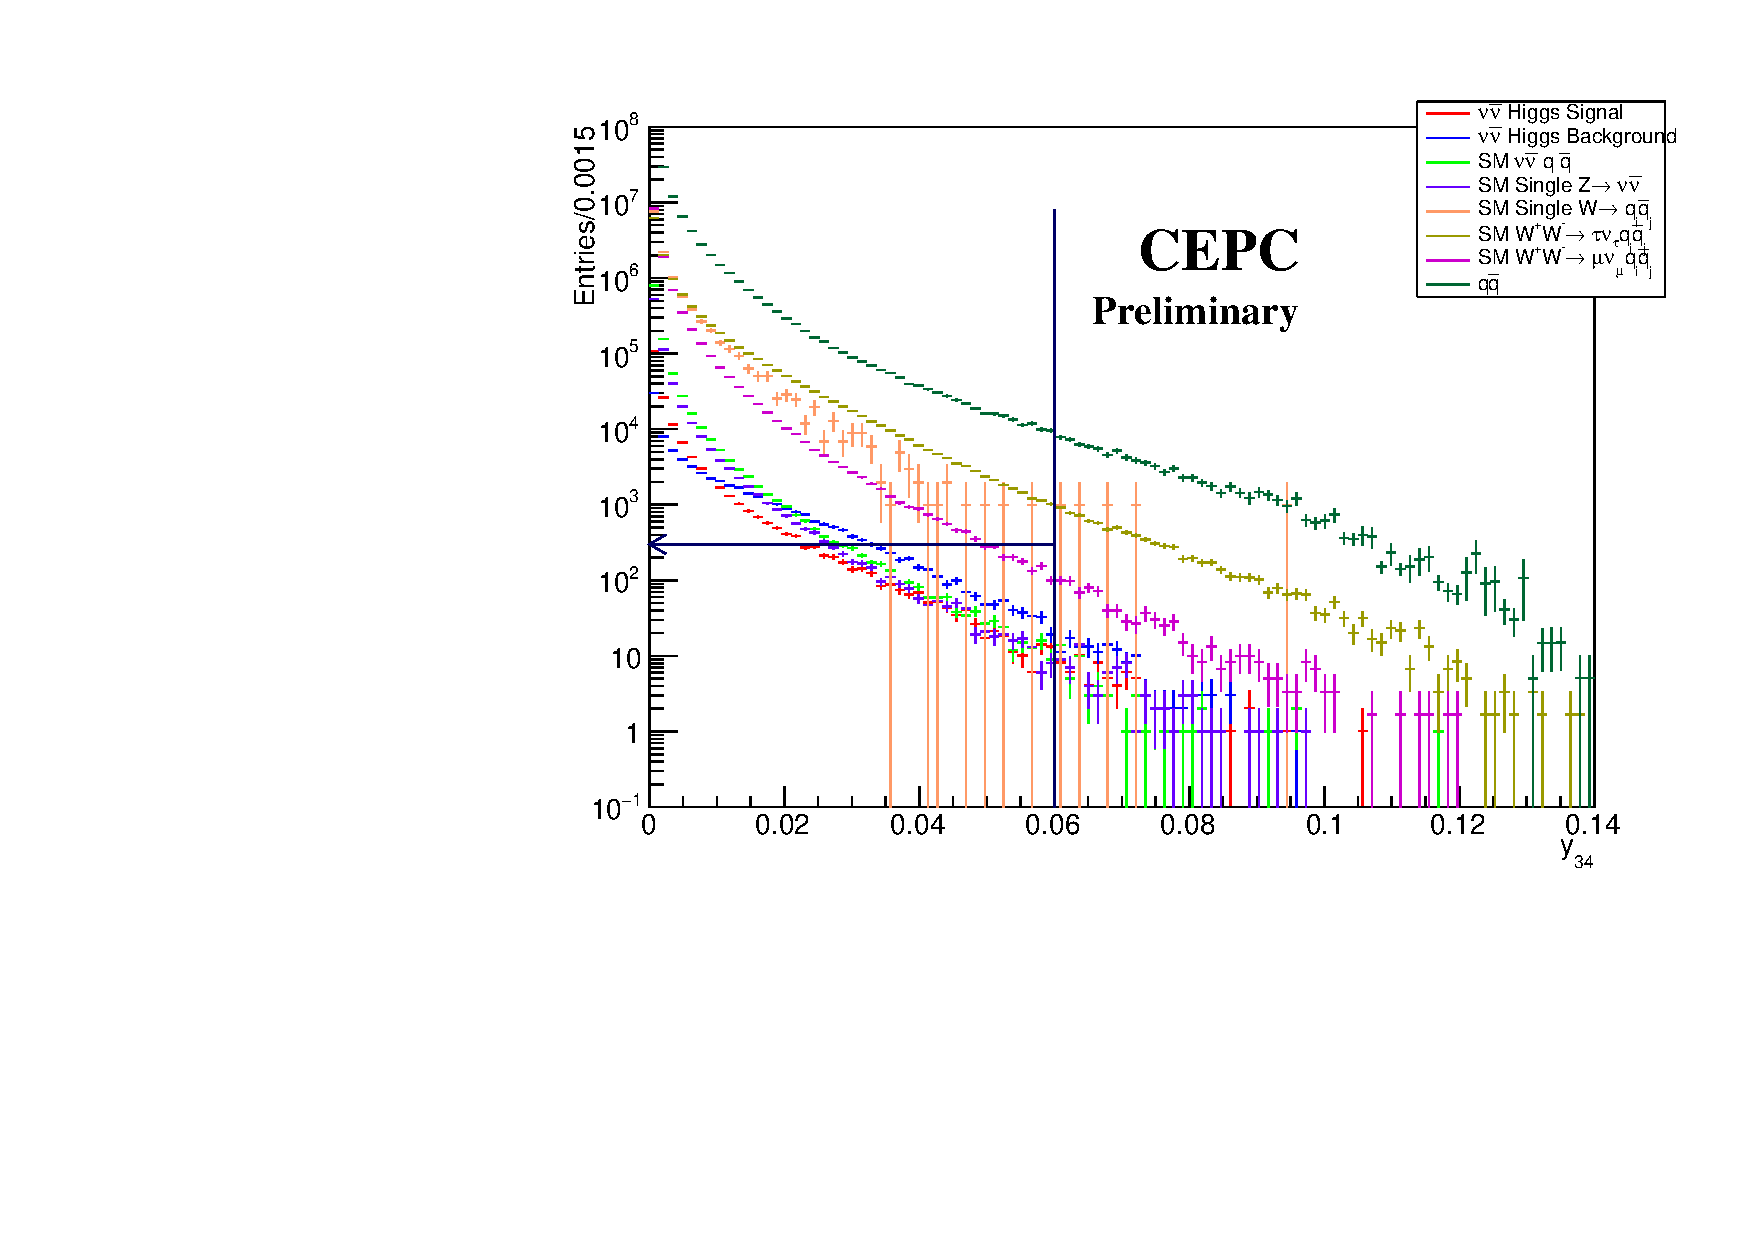
\includegraphics[width=\textwidth]{Analysis/nnh/y34.pdf}
  \end{minipage}
}
\caption{The $y_{12}$(left), $y_{23}$(middle) and $y_{34}$ right distribution in \nnh analysis.}
\end{figure}

\begin{figure}[!htbp]
\label{fig:BDT_nnh}
\centering
\subfigure[]
{
  \begin{minipage}[b]{0.42\textwidth}
  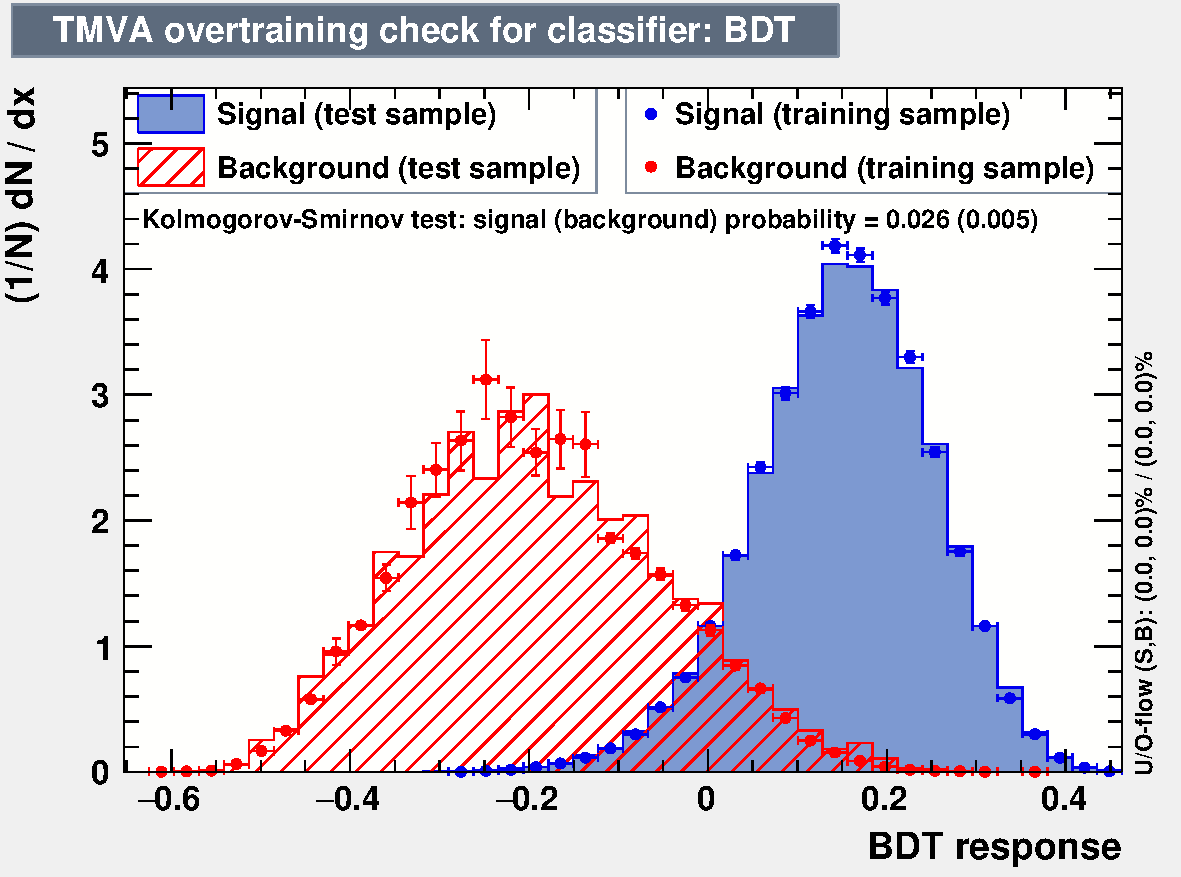
\includegraphics[width=\textwidth]{Analysis/nnh/overtrain_BDT.pdf}
  \end{minipage}   
}
\subfigure[]
{
  \begin{minipage}[b]{0.42\textwidth}
  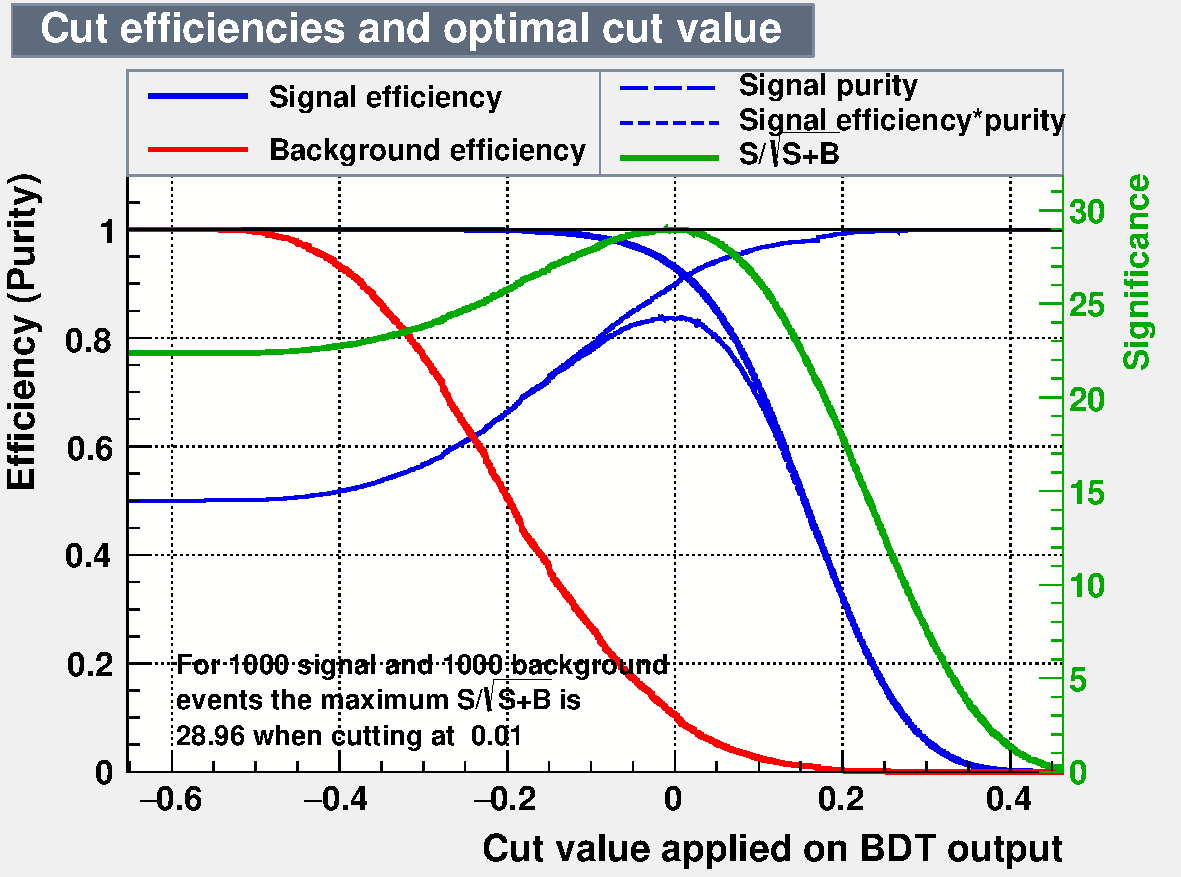
\includegraphics[width=\textwidth]{Analysis/nnh/mvaeffs_BDT.pdf}
  \end{minipage}
}
\caption{Over training check of BDT distribution(left) and optimization of the 
BDT cut performance.}
\end{figure}

\begin{table}[!htbp]
\chuhao
\label{tab:nnh_cut}
\center
\begin{tabular}{c|c|c|c|c|c|c|c|c}\hline
cutflow                 &signal          &\nnh bkg          &zzsl             &sznuqq          &wwsltauq         &wwslmuq           &swslqq           &qq                \\ \hline 
No Cut                  &170633          &76604.1         &\ten{1.08992}{6} &744218          &\ten{1.19114}{7} &\ten{1.19114}{7}  &\ten{1.30255}{7} &\ten{2.46847}{8}  \\ \hline 
2 jets in final state   &170512          &73227.4         &\ten{1.08987}{6} &744201          &\ten{1.19112}{7} &\ten{1.19112}{7}  &\ten{1.30255}{7} &\ten{2.46842}{8}  \\ \hline 
NPFO                    &170349          &42734.8         &980878           &656657          &\ten{1.17604}{7} &\ten{1.16597}{7}  &\ten{1.22262}{7} &\ten{2.39672}{8}  \\ \hline 
$E_{total}$             &152374          &33867.2         &451233           &250618          &\ten{5.06253}{6} &\ten{1.27372}{6}  &\ten{2.07027}{6} &\ten{1.01743}{8}  \\ \hline 
pT                      &142048          &31579.8         &413994           &229568          &\ten{4.31686}{6} &\ten{1.19619}{6}  &\ten{1.93607}{6} &297012            \\ \hline 
IsoLep Veto             &141112          &27966           &410719           &227762          &\ten{3.73815}{6} &365116            &682854           &294929            \\ \hline 
$M_{inv}$               &134583          &26165.2         &41340.5          &23255.3         &\ten{2.20577}{6} &66320             &336493           &111687            \\ \hline 
$M_{recoil}$            &125958          &24817.4         &37889.9          &20720.1         &\ten{1.75479}{6} &29908             &237815           &85653.4           \\ \hline 
y12                     &125228          &24164.8         &37138.4          &20306.8         &\ten{1.61702}{6} &27807.4           &228934           &83451.1           \\ \hline 
y23                     &126365          &13478.1         &29136.3          &15976.7         &\ten{1.07172}{6} &18577.8           &126308           &71353             \\ \hline 
y34                     &107347          &5708.84         &26728            &14616.3         &889531           &16016             &110520           &69372.9           \\ \hline 
costheta                &104023          &5169.31         &21169.6          &11891.4         &506063           &9354.92           &85850.1          &48209.6           \\ \hline 
BDT Cut                 &83852.1         &1961.65         &2704.18          &1566.07         &11116.3          &476.269           &986.783          &6170.45           \\ \hline         
\end{tabular}
\caption{Signal and background yields in the cutflow of \nnh analysis, normalized to 5000 \ifb}
\end{table}

%\clearpage




\subsection{$\qqh$ Event Seleciton} 
The $\qqh$ channel refers to $ZH$ production in which both $Z$ and Higgs bosons decays hadronically.
We require exclusively 4 jets reconstructed by Durham-like algorithm\cite{Durham} in final states, corresponding to the leading logrithm approximation of 4-partners final states. The domiant SM backgrounds are consist of diboson production followed by hadronic decays of both bosons, and quark pair production. Events with loosened isolation lepton candidates were rejected.
All of the 4 jets are required to contain at least 10 PFOs to remove the 
events with fake jets. 
The visible energy of each event are required to be larger than 206 \GeV 
to reject the events with energetic nuetrinos. 
In figure \ref{fig:VisEn_nPFO} visible energy and minimum PFO multicplicity of the jets distributions of signal and backgrounds are presented.\par
\begin{figure}
\label{fig:VisEn_nPFO}
\centering
\subfigure[]
{
  \begin{minipage}[b]{0.42\textwidth}
  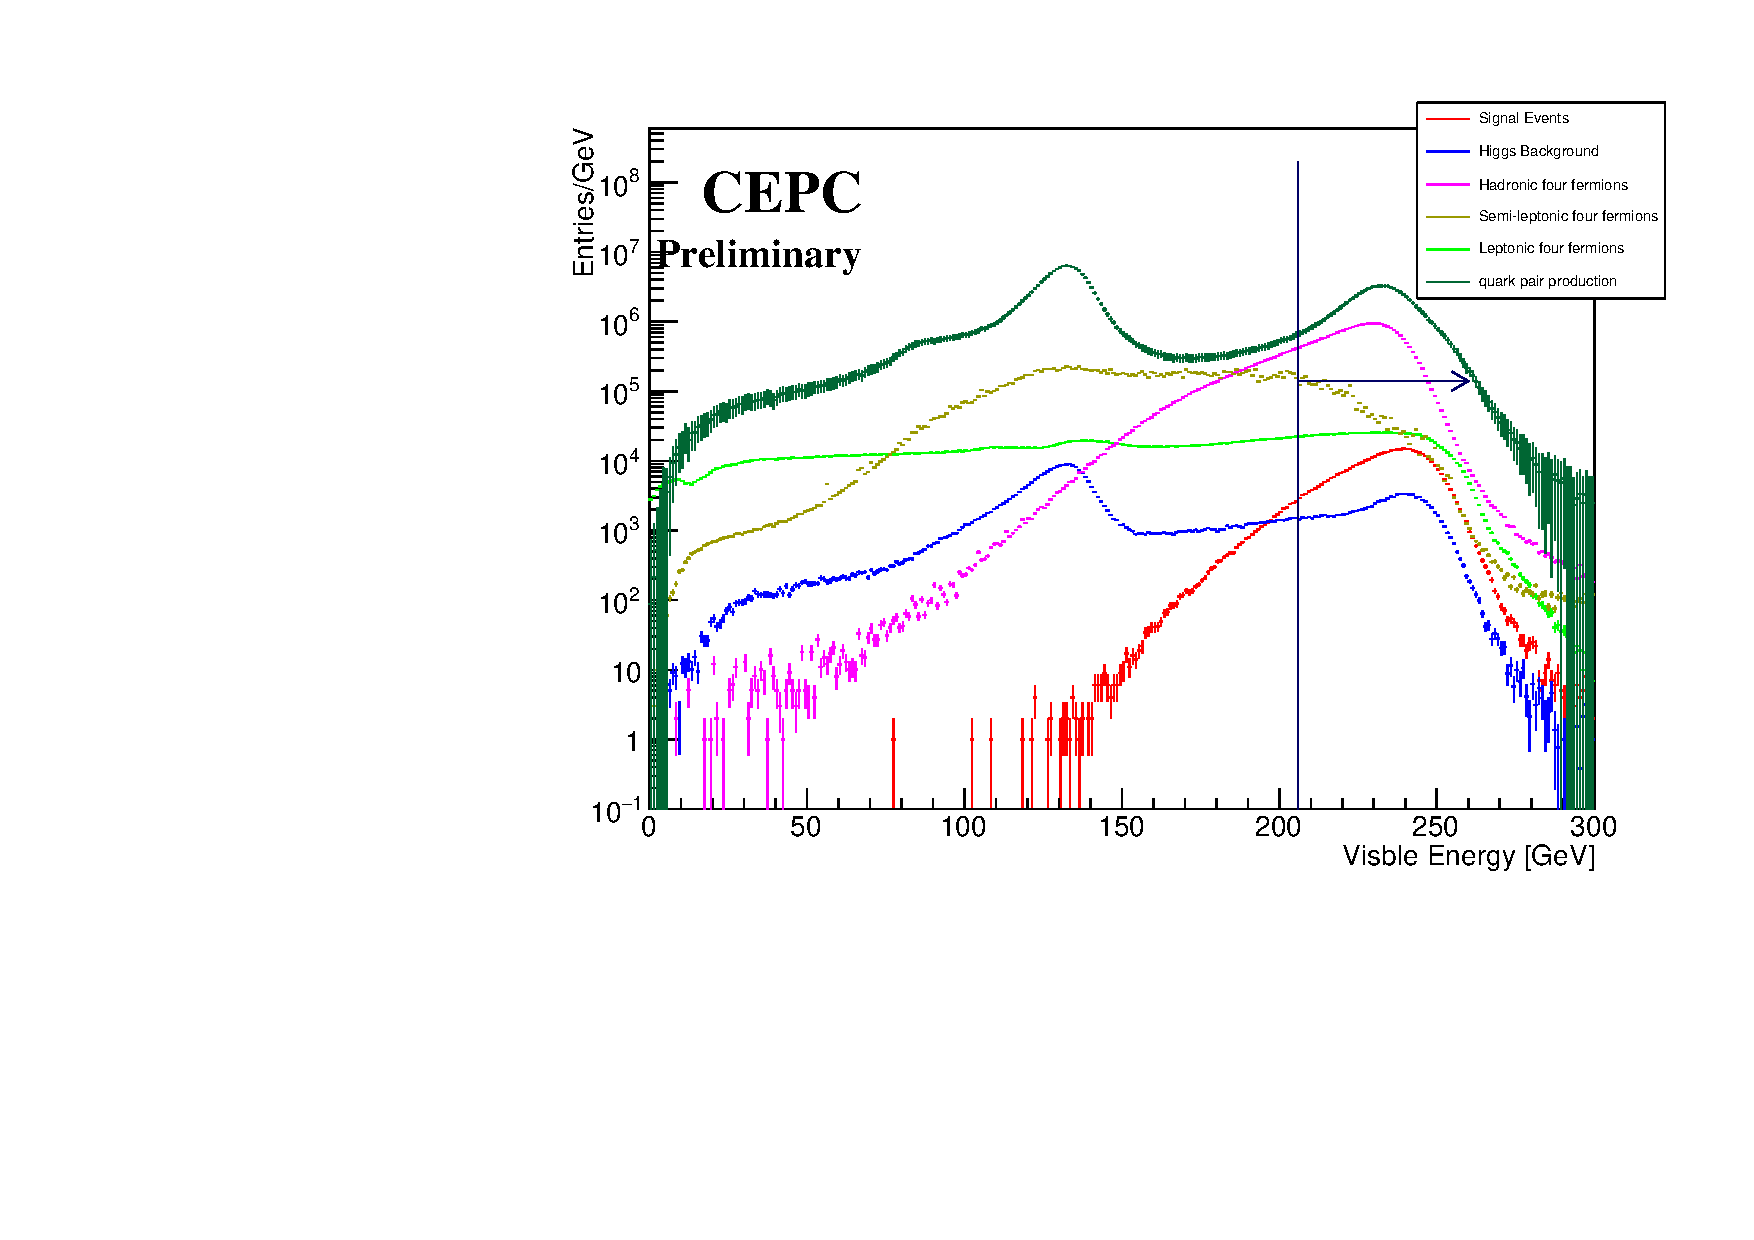
\includegraphics[width=\textwidth]{Analysis/qqh/VisEn.pdf}
  \end{minipage}
}
\subfigure[]
{
  \begin{minipage}[b]{0.42\textwidth}
  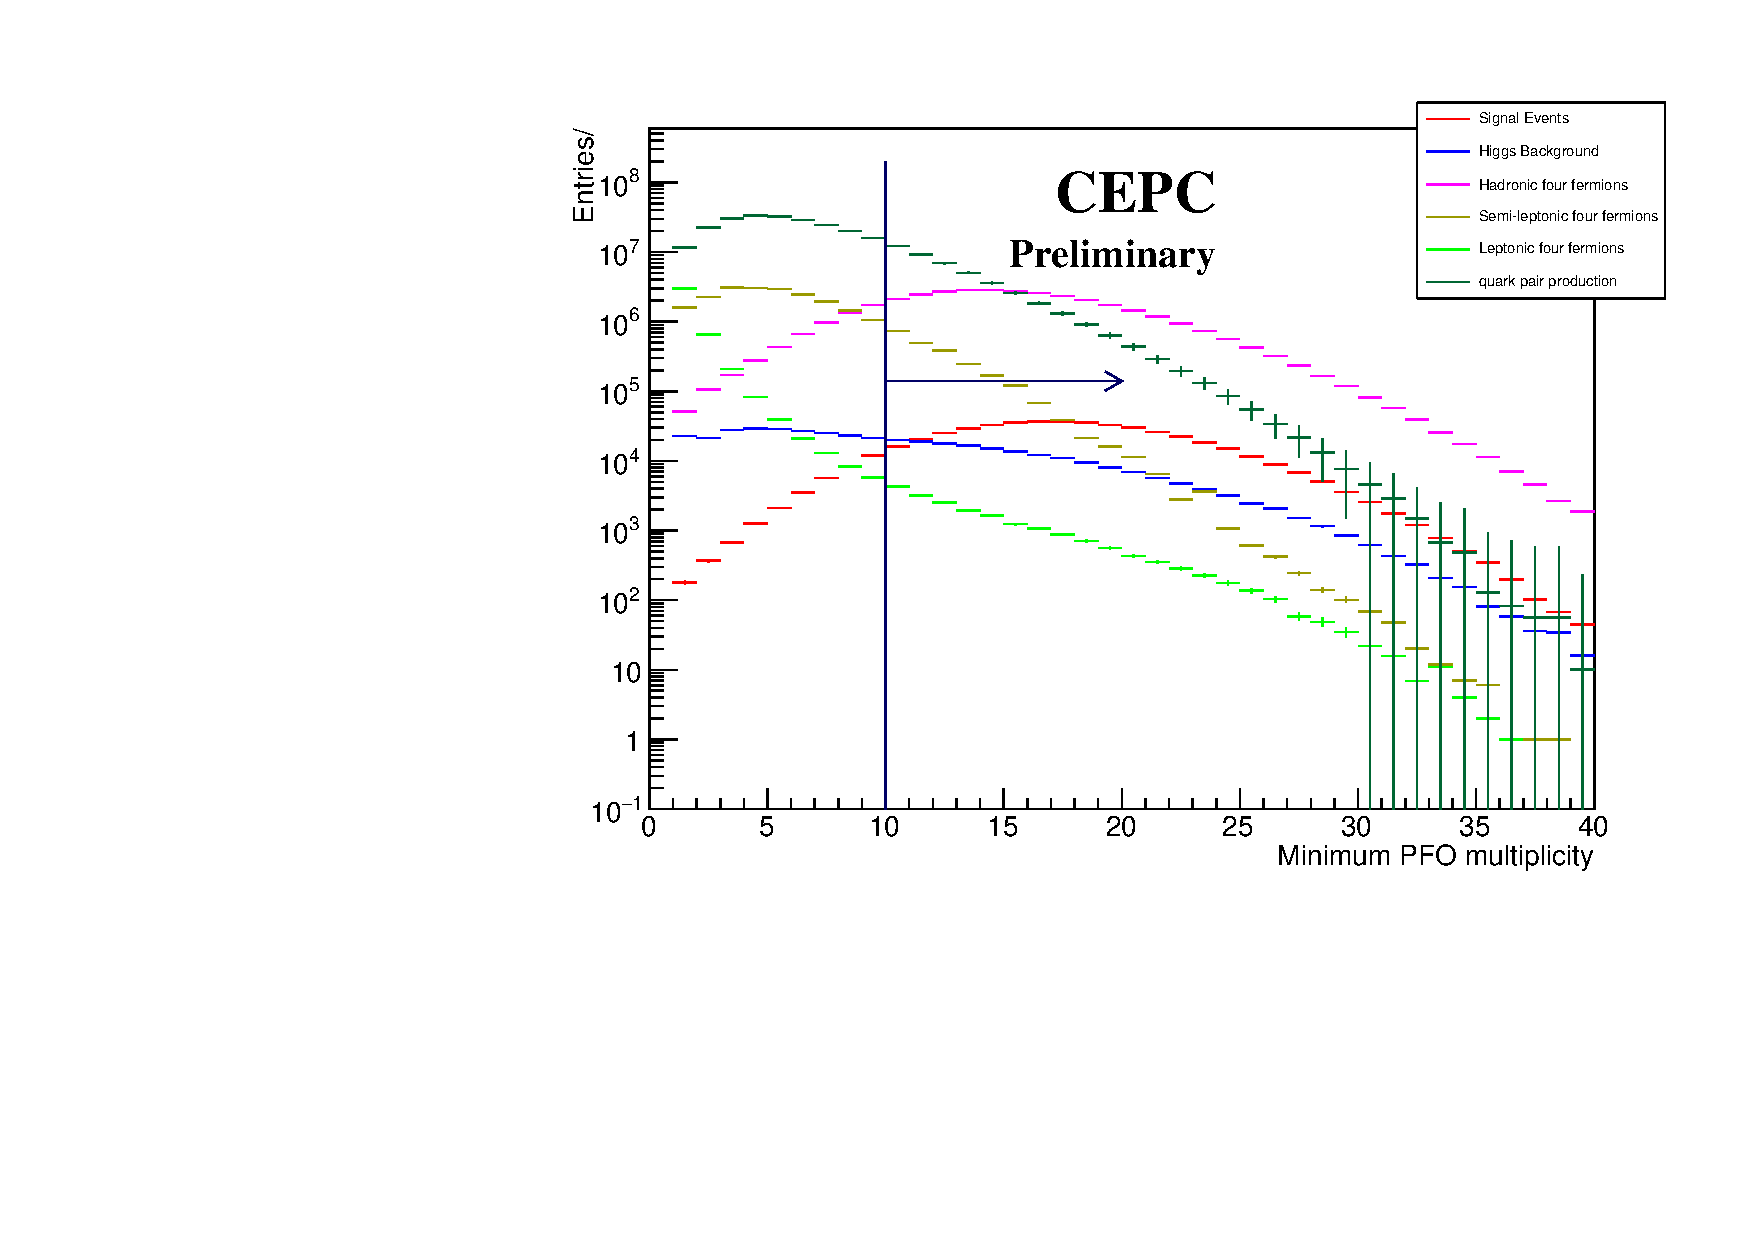
\includegraphics[width=\textwidth]{Analysis/qqh/nPFOmin.pdf}
  \end{minipage}
}
\caption{Distribution of visible energy(left) and minimum jets' pfo multiplicity(right) for the signal and SM backgrounds.}
\end{figure}


%It can also effectively remove the 2 fermions events with radiation return, since emitted photon can be missed from detection.

%To further suppress the background from 2 jets events, two variable are used as discriminator. One is called yth-value('th' refer to 3 and 4 here) which is constructed from PFO distributionthe other one is called sphericity, which represents the PFO distribution shape in each event. The distribution of \emiss, $y_34$ and sphericity can be found in figure \ref{fig:missingE}.
To suppress the background from 2 jets events, the $y_{34}$ are used as discriminator, which can effectively select the 4 jets events 
from those with lower jet multiplicity. A cut on the energetic-weighted angular 
dispersion was defined as $\Delta\theta$ variable, 
which was used in ALEPH 4-bjets channel analysis\cite{ALEPH_ZH_PLB}, is also used to furuther suppress the $q\bar{q}$ and semi-leptonic 4 fermions backgrounds.
 . The distribution of $y_{34}$ and $\Delta\theta$ can be found in figure 
 \ref{fig:y34_Deltatheta}.
 \begin{figure}
\label{fig:y34_Deltatheta}
\centering
\subfigure[]
{
  \begin{minipage}[b]{0.42\textwidth}
  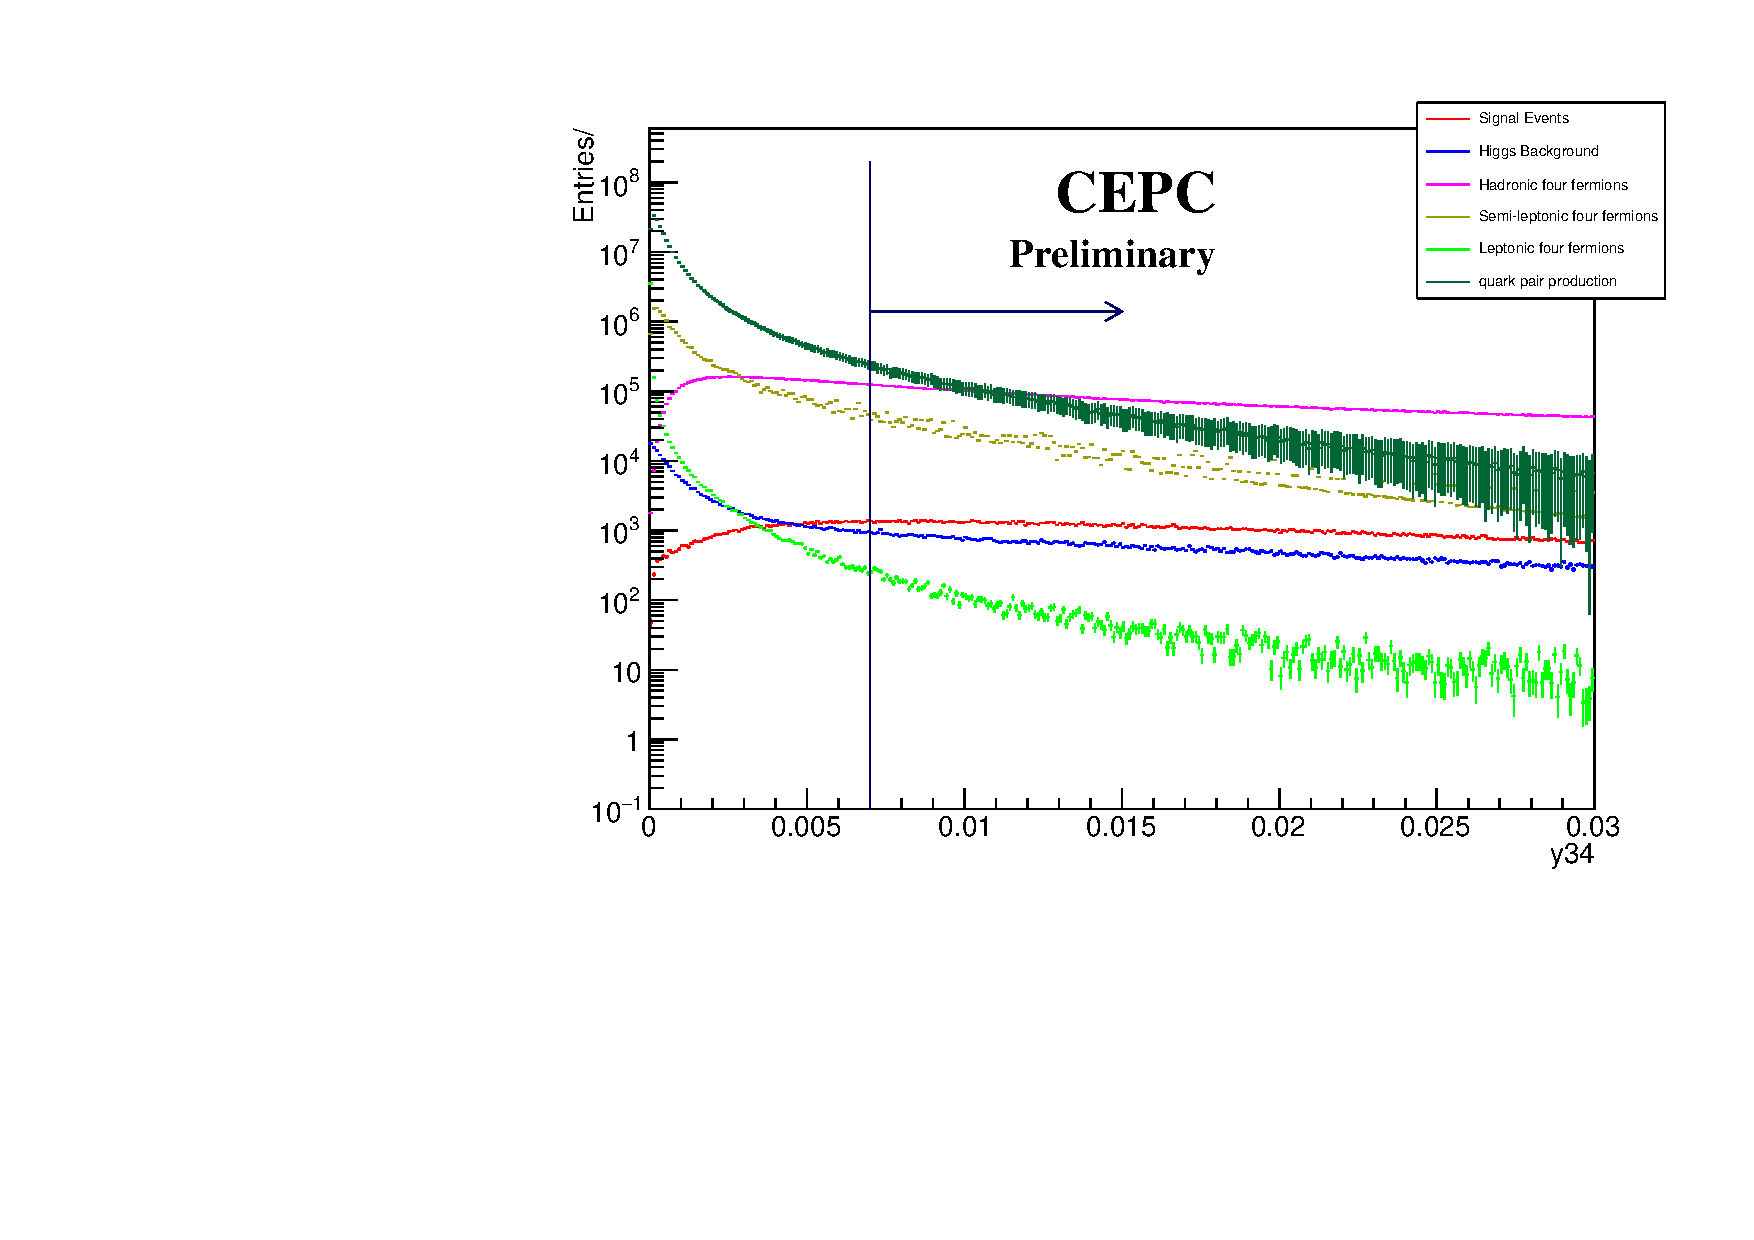
\includegraphics[width=\textwidth]{Analysis/qqh/y34.pdf}
  \end{minipage}
}
\subfigure[]
{
  \begin{minipage}[b]{0.42\textwidth}
  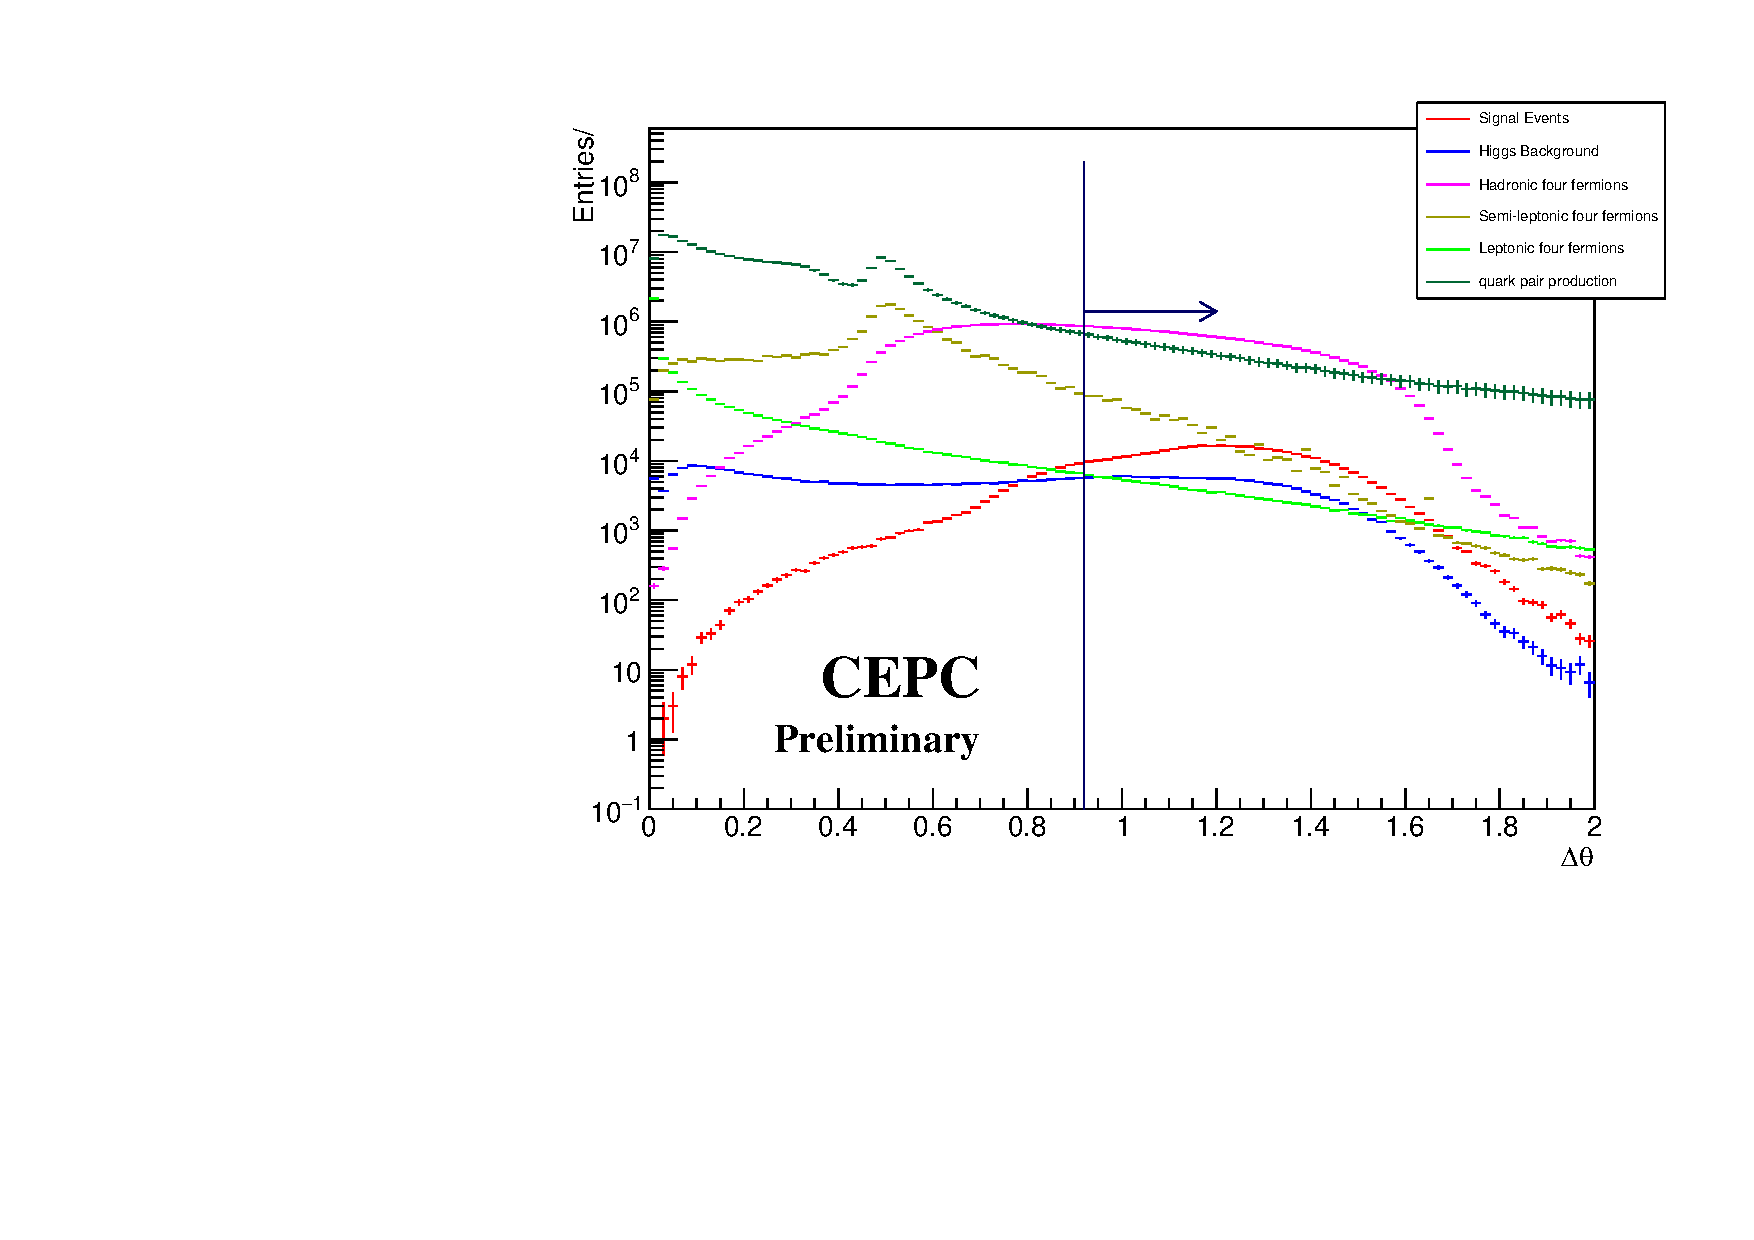
\includegraphics[width=\textwidth]{Analysis/qqh/DeltaTheta.pdf}
  \end{minipage}
}
\caption{Distribution of $y_{34}$(left) and $\Delta\theta$ (right) for the signal and SM backgrounds.}
\end{figure}
 \par 
%\begin{figure}[htpb]
%\centering
%    \includegraphics[width=0.45\textwidth]{figures/MissingE.pdf}
%    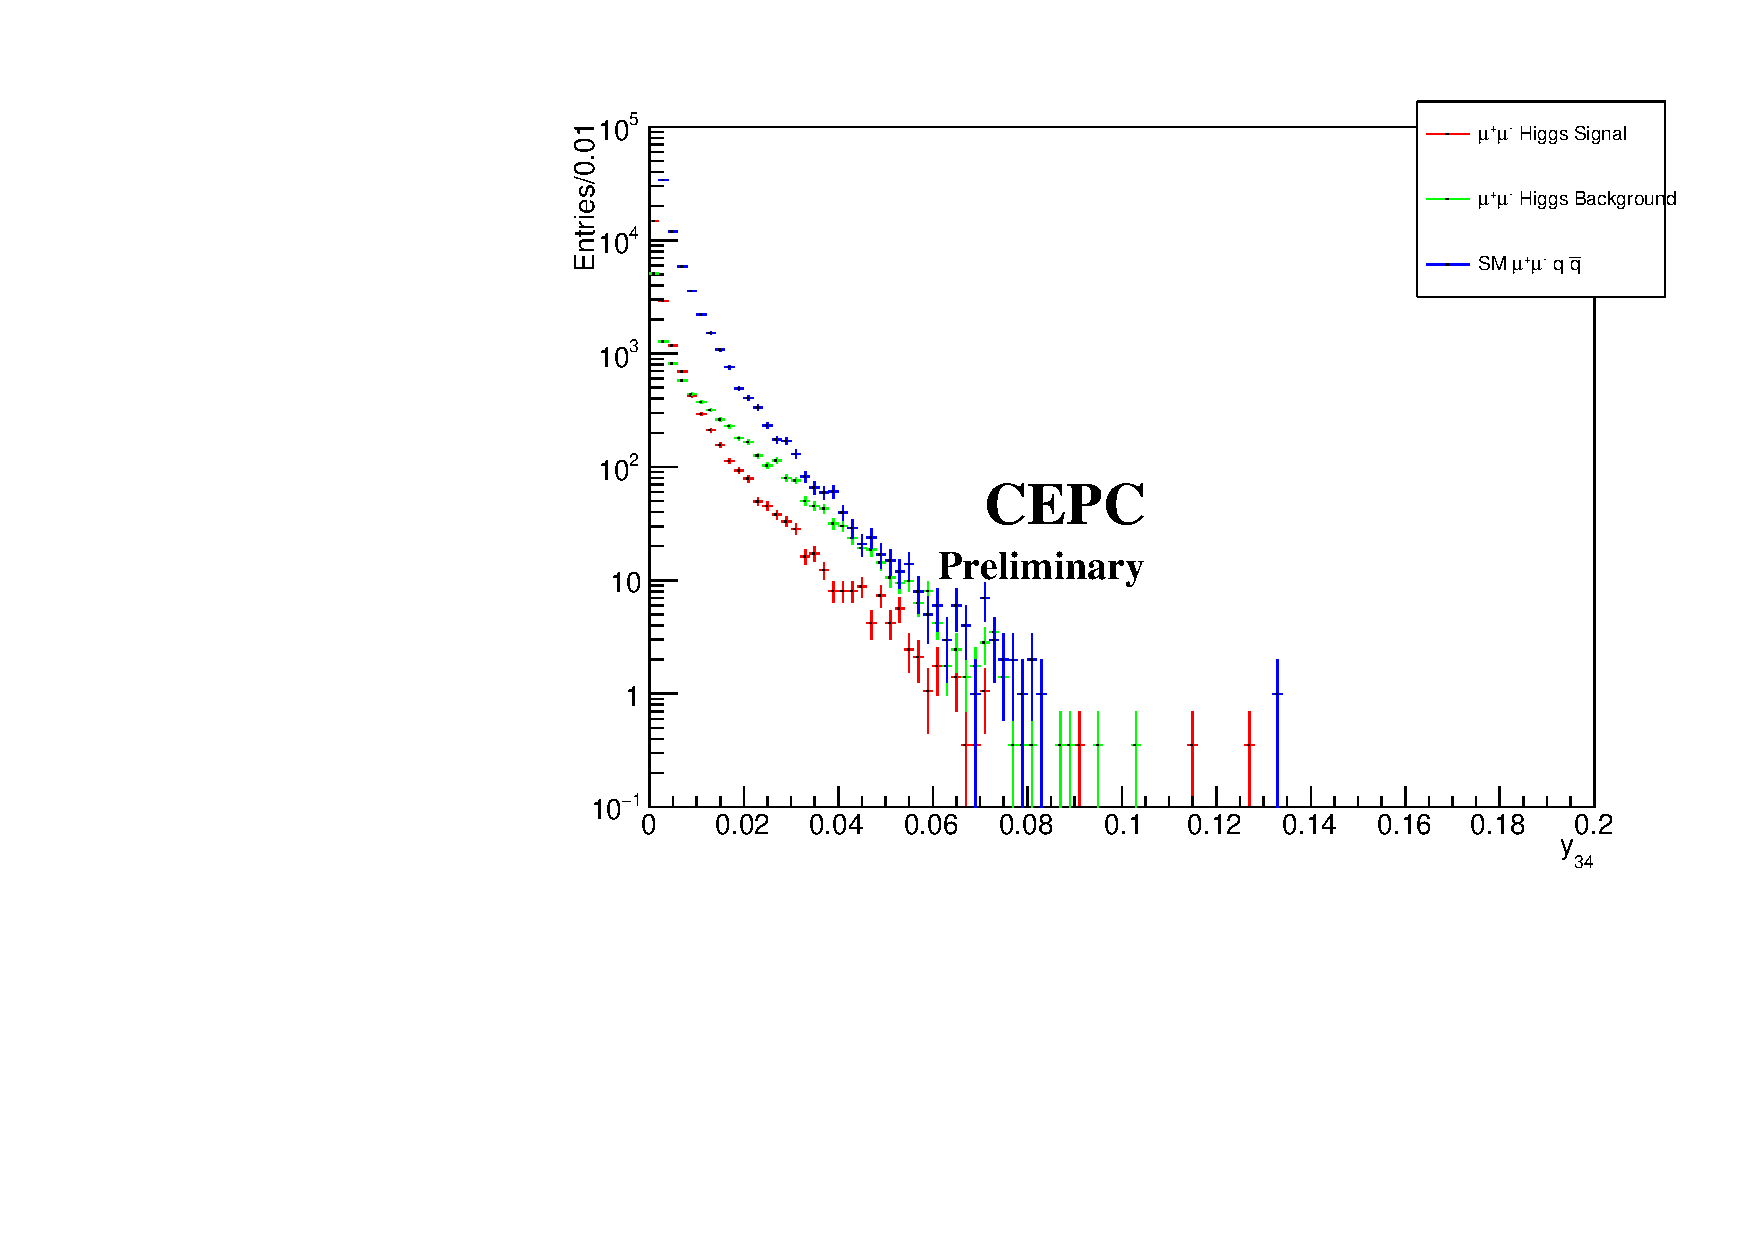
\includegraphics[width=0.45\textwidth]{figures/y34.pdf}
%    \includegraphics[width=0.45\textwidth]{figures/Sphericity.pdf}
%\caption{Distribution of MissingE, $y_{34}$ and sphericity of signal and background events, normalized to 5000 fb$^{-1}$
%}
%\label{fig:missingE}
%\end{figure}

The 4 jets in the final states are paired in order to get minimum $\chi^2$ defined as:
\begin{equation}
     \chi^2_{HZ} = \mathrm{min}\{(m_{ij}-m_H)/\sigma^2_{H} + (m_{kl}-m_Z)/\sigma^2_{Z} \}
     \label{for:chi2}
\end{equation}
in which i,j,k,l are the jet index, running from 1-4; $m_{ij}$ is the invariant mass of one jet pair and $m_{kl}$ is that of another pair; $m_H$ and $m_Z$ are Higgs and Z boson mass; $\sigma_H$ and $\sigma_Z$ are the width of reconstructed jet pair invariant mass from Higgs and  $Z$ boson. A variable $\chi^2_{WW}$ is defined in the similar way as formula \ref{for:chi2}, in which the $Z$/Higgs masses and widths are replaced by those of $W$ boson. The $\chi^2_{HZ}$ and $\chi^2_{ZZ}$ are combined into a variable $X$:
\begin{equation}
  X = \dfrac{\chi^2_{WW}-\chi^2_{HZ}}{chi^2_{WW}+\chi^2_{HZ}}
  \label{for:X}
\end{equation}
 The X value distrutes in the range from -1 to 1. For signal events, it tends to be positive 
 values(close to 1) while for the dominant $WW$ hadronic background, the X value tends to be negative(close to -1), as shown in figure \ref{fig:X}. Thus X provides discrimination power against $WW$ hadronic events.
 \begin{figure}
 \label{fig:X}
 \centering
 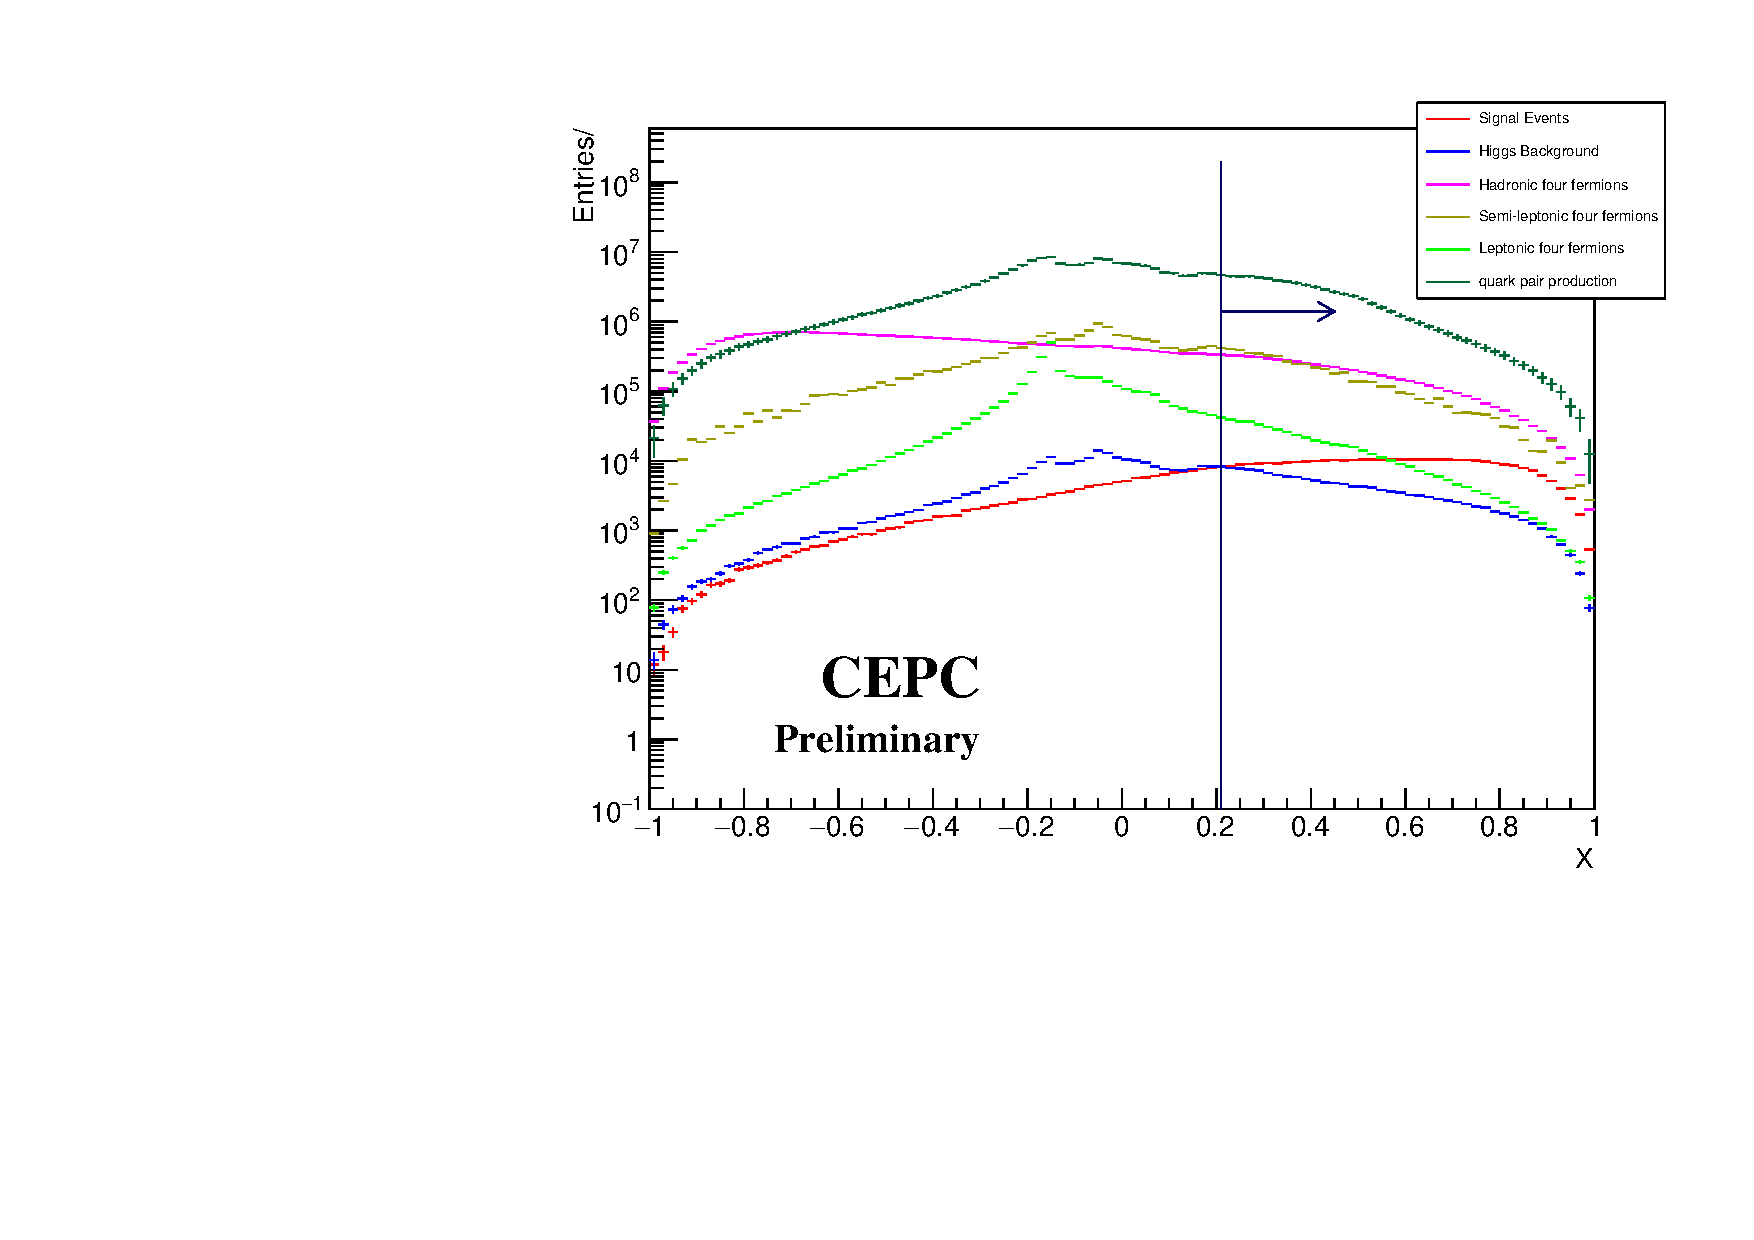
\includegraphics[width=0.67\textwidth]{Analysis/qqh/X.pdf}
 \caption{The distribution of $X$ defined in formula \ref{for:X}.}
 \end{figure}
\par
%invariant mass distribution of 2 jets from Higgs or Z correspondingly.  The distribution of 2 jet pair invariant mass can be found in figure \ref{fig:jet_pair_invmass}
%\begin{figure}[htpb]
%\centering
%    \includegraphics[width=0.45\textwidth]{figures/HZ_signal.eps}
%    \includegraphics[width=0.45\textwidth]{figures/HZ_4q.eps}
%\caption{Distribution of invariant mass of the two jet pairs for signal(left) and WW(right) events. The x-axis represents the invariant mass of a jet pair which is cloest to the higgs among all combination; the y-axis represents the invariant mass of another jet pair.
%}
%\label{fig:jet_pair_invmass}
%\end{figure}

%The results of the cutflow are summerized in table \ref{tab:cutflow}.
%\begin{table}[!htbp]
%\centering
%\begin{tabular}{|c|c|c|c|c|c|c|c|c|c|} \hline
%         &   signal   & other qqH      &  ffH   &  qq   &  ll   &  qqqq  &   llqq   &  lvqq   & vvqq  leptonic \\ \hline
%Dataset  &  \multicolumn{2}{c|}{724k}  &  405k  & 250M  & 20.4M & 36.9M  &  3.2M    &  36.45M &  2.17M    \\ \hline
%  4J FS  &  494.6k    &   214.2k       & 299.4k &\multicolumn{2}{c|}{267.1M}
%                                                                & 36.85M &  3.16M   &  35.9 M & 1.36M   \\ \hline
%  Iso Lep Veto
%         & 489.7k     &   154.4k       & 130.9k &\multicolumn{2}{c|}{242.2M}
%                                                                & 36.2M  & 558.4k   &  9.33M  & 1.35M     
%                                                                \\ \hline
%  \emiss$<$76 GeV
%         & 487.3k     &   130.2k       & 15.9k  &\multicolumn{2}{c|}{238.8M}
%                                                                & 36.11M & 354.5k   &  3.1M   & 964         \\ \hline
%  $y_{34}>$0.013
%        & 339.1k     &  99.34k        & 8.71k  &\multicolumn{2}{c|}{12.58M}
%                                                                & 20.83M & 78.25k   & 345.2k  & 88      \\ \hline
%  sphericity$>$0.44
%        & 315.1k     &  92.8k         & 7.87k  &\multicolumn{2}{c|}{2.88M}
%                                                                & 16.84M & 56.1k    & 194.5k  & 34    \\   \hline
%  Min($\chi^2 <$18) 
%        & 240.7k     & 61.7k         & 2.6k   &\multicolumn{2}{c|}{1.69M}
%                                                                & 10.1M  & 15.96k   & 13.52k  &  0   \\ \hline                                                  
%                                                                            
%     
%\end{tabular}
%\caption{ Event yields of signal and background in cutflow, normalized to 5000 fb$^{-1}$} 
%\label{tab:cutflow}
%\end{table}
The BDT\cite{BDT} method is applied to further suppress the SM backgrounds. The variables like 
reconstructed Higgs and $Z$ mass, different combination of jet pair invariant masses, $y_{34}$ 
and $y_{45}$ and sphericity, reconstructed $Z$ and Higss $\cos \theta$ and highest energy of 
of jets are used in the training. Figure \ref{fig:qqh_BDT} shows the signal and background distribution of linear correlation of these variables and the outcome BDT response of signal and backgrounds.
\begin{figure}
\label{fig:qqh_BDT}
\centering
\subfigure[]
{
  \begin{minipage}[b]{0.42\textwidth}
  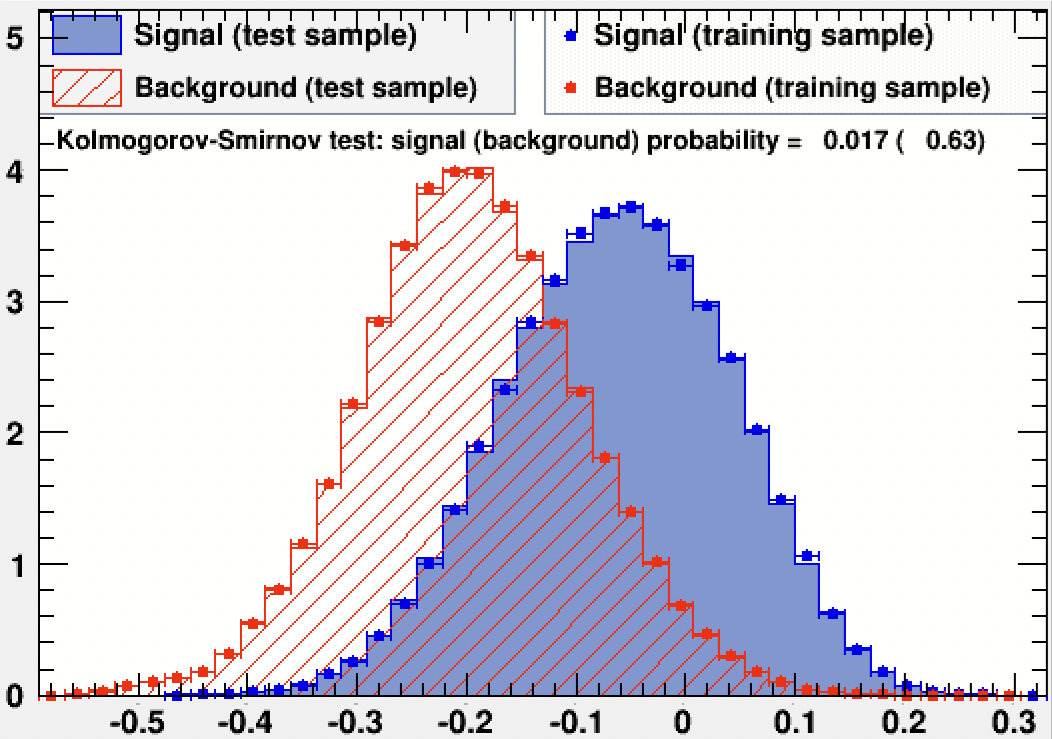
\includegraphics[width=\textwidth]{Analysis/qqh/BDT.png}
  \end{minipage}
}
\subfigure[]
{
  \begin{minipage}[b]{0.42\textwidth}
  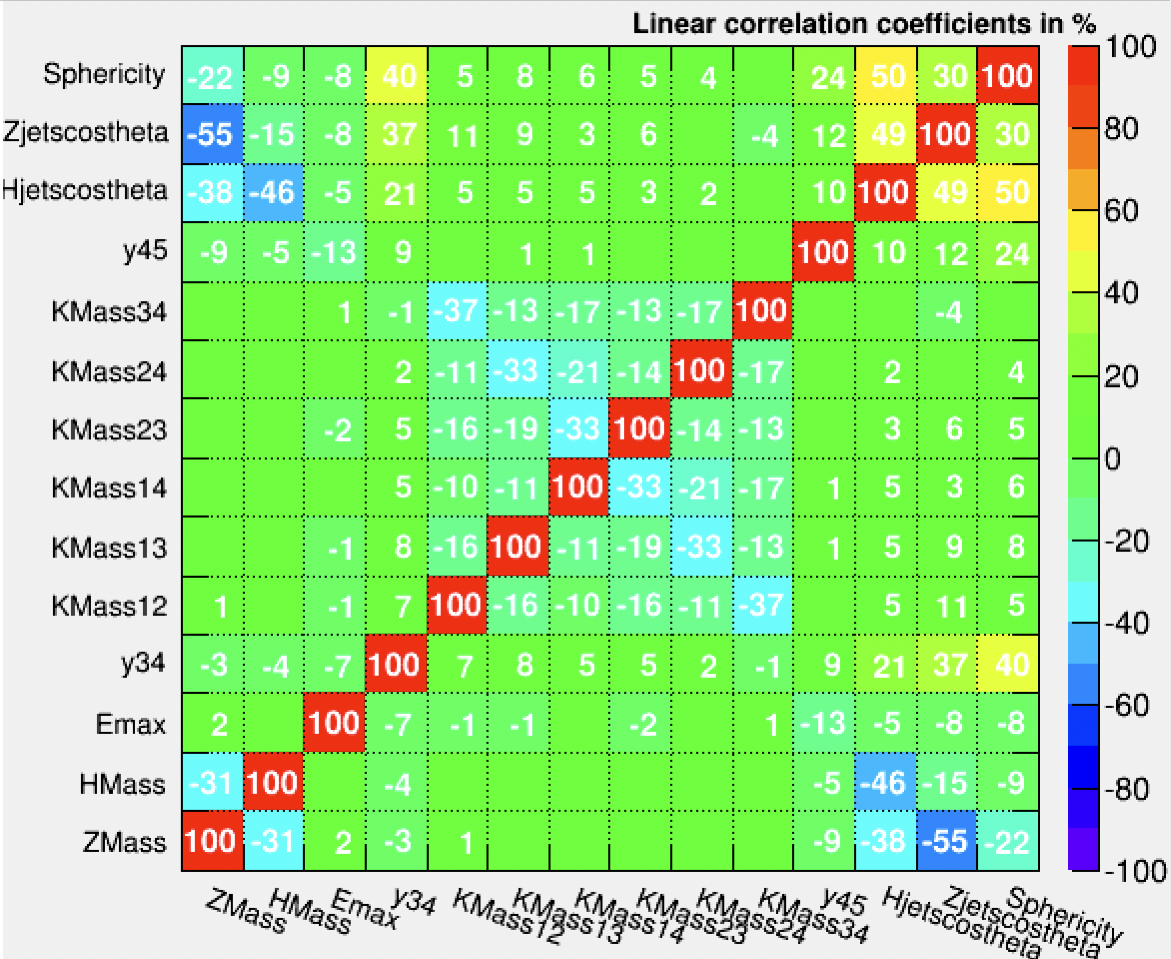
\includegraphics[width=\textwidth]{Analysis/qqh/Correlation.png}
  \end{minipage}
}
\caption{Linear correlation map of variables used in BDT training(left) and the outcome BDT 
response of signal and backgrounds.}
\end{figure}


\begin{table}[!htpb]
\centering
\chuhao
\begin{tabular}{c|c|c|c|c|c|c|c|c|c}\hline
         & \tabincell{c}{signal \\ combined}   &  $\Hboson \to \bpair$   & $\Hboson\to\cpair$   & $\Hboson\to\gpair$   & \tabincell{c}{background\\ combined} & \tabincell{c}{higgs \\background}   &   \tabincell{c}{4 fermions\\ hadronic}&  quark pair &  \tabincell{c}{4 fermion\\ semi-leptonic}  \\ \hline 
 4 jets and iso-lepton veto 
         &  493947 & 413299   & 19362  & 61286  &     75 M      &  299583  &  36.83 M &   23.86M   &   14.72 M      \\ \hline
  $E_{vis} > $206 GeV
         &  459972 &  381470  & 18690  & 59812  &     50.6 M    &  109529  &  28.19 M  &  20.37M  &  1.967M  \\ \hline
 $y_{34} > 0.007$
         &  393979 &  325137 &   15976  & 52866 & 26.4 M        &   100813 &  21.32 M  &  5.207 M  &  218394 \\ \hline
 $N_{jet,pfo} \ge 9$
         &  371240 &  305982 &   14903  & 50355 & 21.4 M        &    82281 &  18.78 M  & 
2.601 M  &  27487  \\ \hline
 $\Delta \theta > $0.92
         &  318163 &  261808 &   12610  & 43745 & 13.55 M       &    71987 &  12.16 M &  
1.315 M  &  4745   \\ \hline
   $X > 0.21$
         &  236652 &  197510 &    9562  & 29580 & 3.15 M        &    38579 &  2.2 M   &  907188   &  3012   \\ \hline
   $BDT > $-0.19
         &  211281 &  177447 &    8324  & 25510 & 1.52 M        &    32653 &  1.08 M  & 
405567   &  580    \\ \hline   
      
\end{tabular}
\caption{Signal and background yields of cutflow in \qqh analysis, normalized to 5000 \ifb}
\label{tab:cut_qqh}
\end{table}


A yth-value is defined according to the PFOs distribution to suppress the background from di-jet events. 

\section{Measurement of $H\to \bpair/\cpair/\gpair$}\label{sec:templatefit}
After applying cuts on jets, the $H\to \bpair/\cpair/\gpair$ are mixed. 
Flavor tagging is necessary to distinguish different flavor final states. 
Based on the high performance flavor tagging algorithm, 
a flavor tagging template fit method is used to simultaneously extract the 
event number of each flavor final state. 
These template fits are cooperated with 
lepton pair recoil mass fit, making the dominant background estimation  
model indepdent. In the following text, the flavor tagging techniques, 
flavor tagging template fit and the 3D flavor tagging-recoil mass fit will 
be described.
\subsection{Flavor tagging}\label{subsec:flavortagging}
 A TMVA based algorithm are implemented to distinguish the jets' flavor. 
 The reconstructed jets are categorized according to the secondary vertex mulitiplicity. 
 In each category, a b-tagging and a c-tagging training with BDT method was implemented over $Z-$pole di-jet events, employing variables including jets kinematic varibles, tracks' impact parameters and secondary vertex information. The training output gives a b-jet likeness weight and a c-jet likeness weight for each jet, representing the resemblance of the jet to a b-jet or a c-jet. The performance of b-tagging and c-tagging is presented in figure \ref{fig:FT_performance}. 
\begin{figure}[!htpb]
\label{fig:FT_performance}
\centering
\subfigure[]
{ 
   \begin{minipage}[b]{0.47\textwidth}
   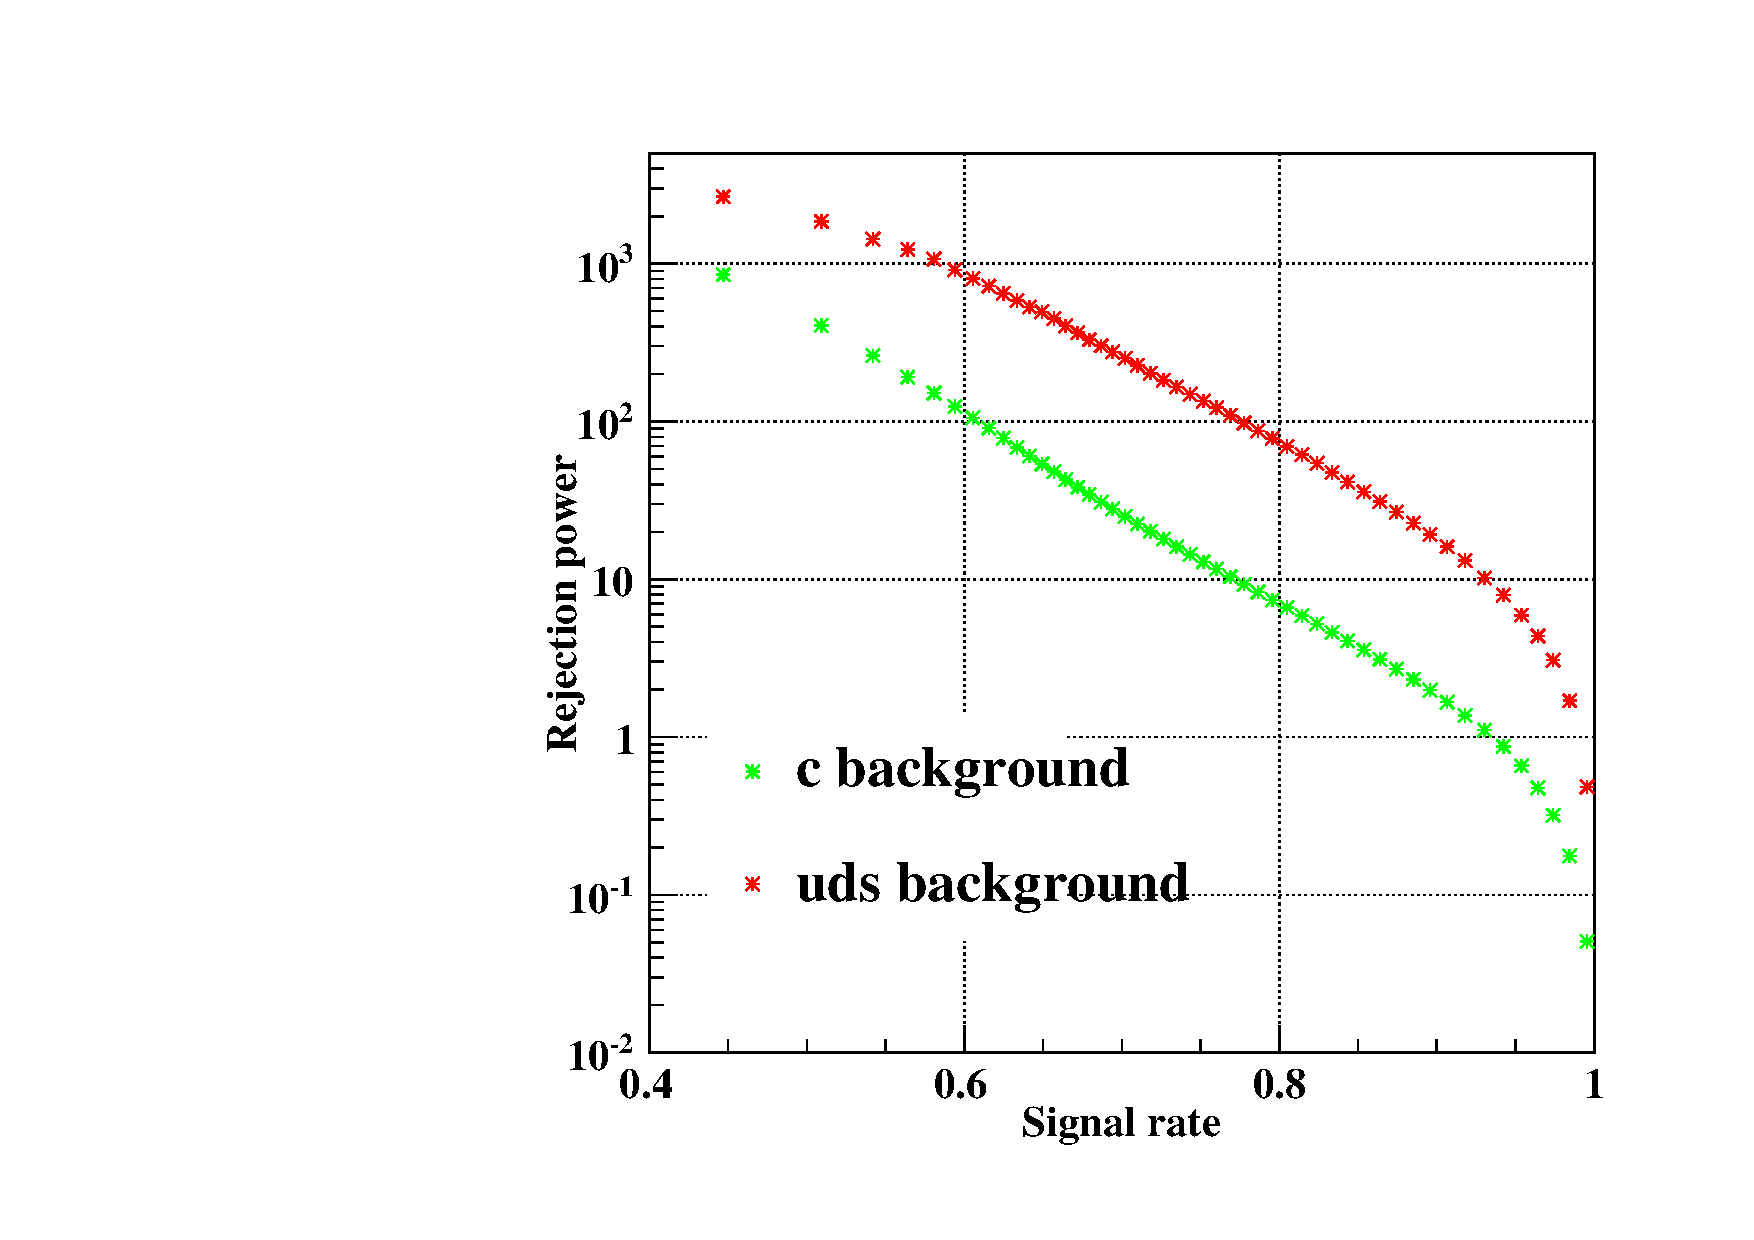
\includegraphics[width=\textwidth]{Btagging/rejectionB-lcfiweights-test.pdf}
   \end{minipage}
}
\subfigure[]
{
    \begin{minipage}[b]{0.47\textwidth}
    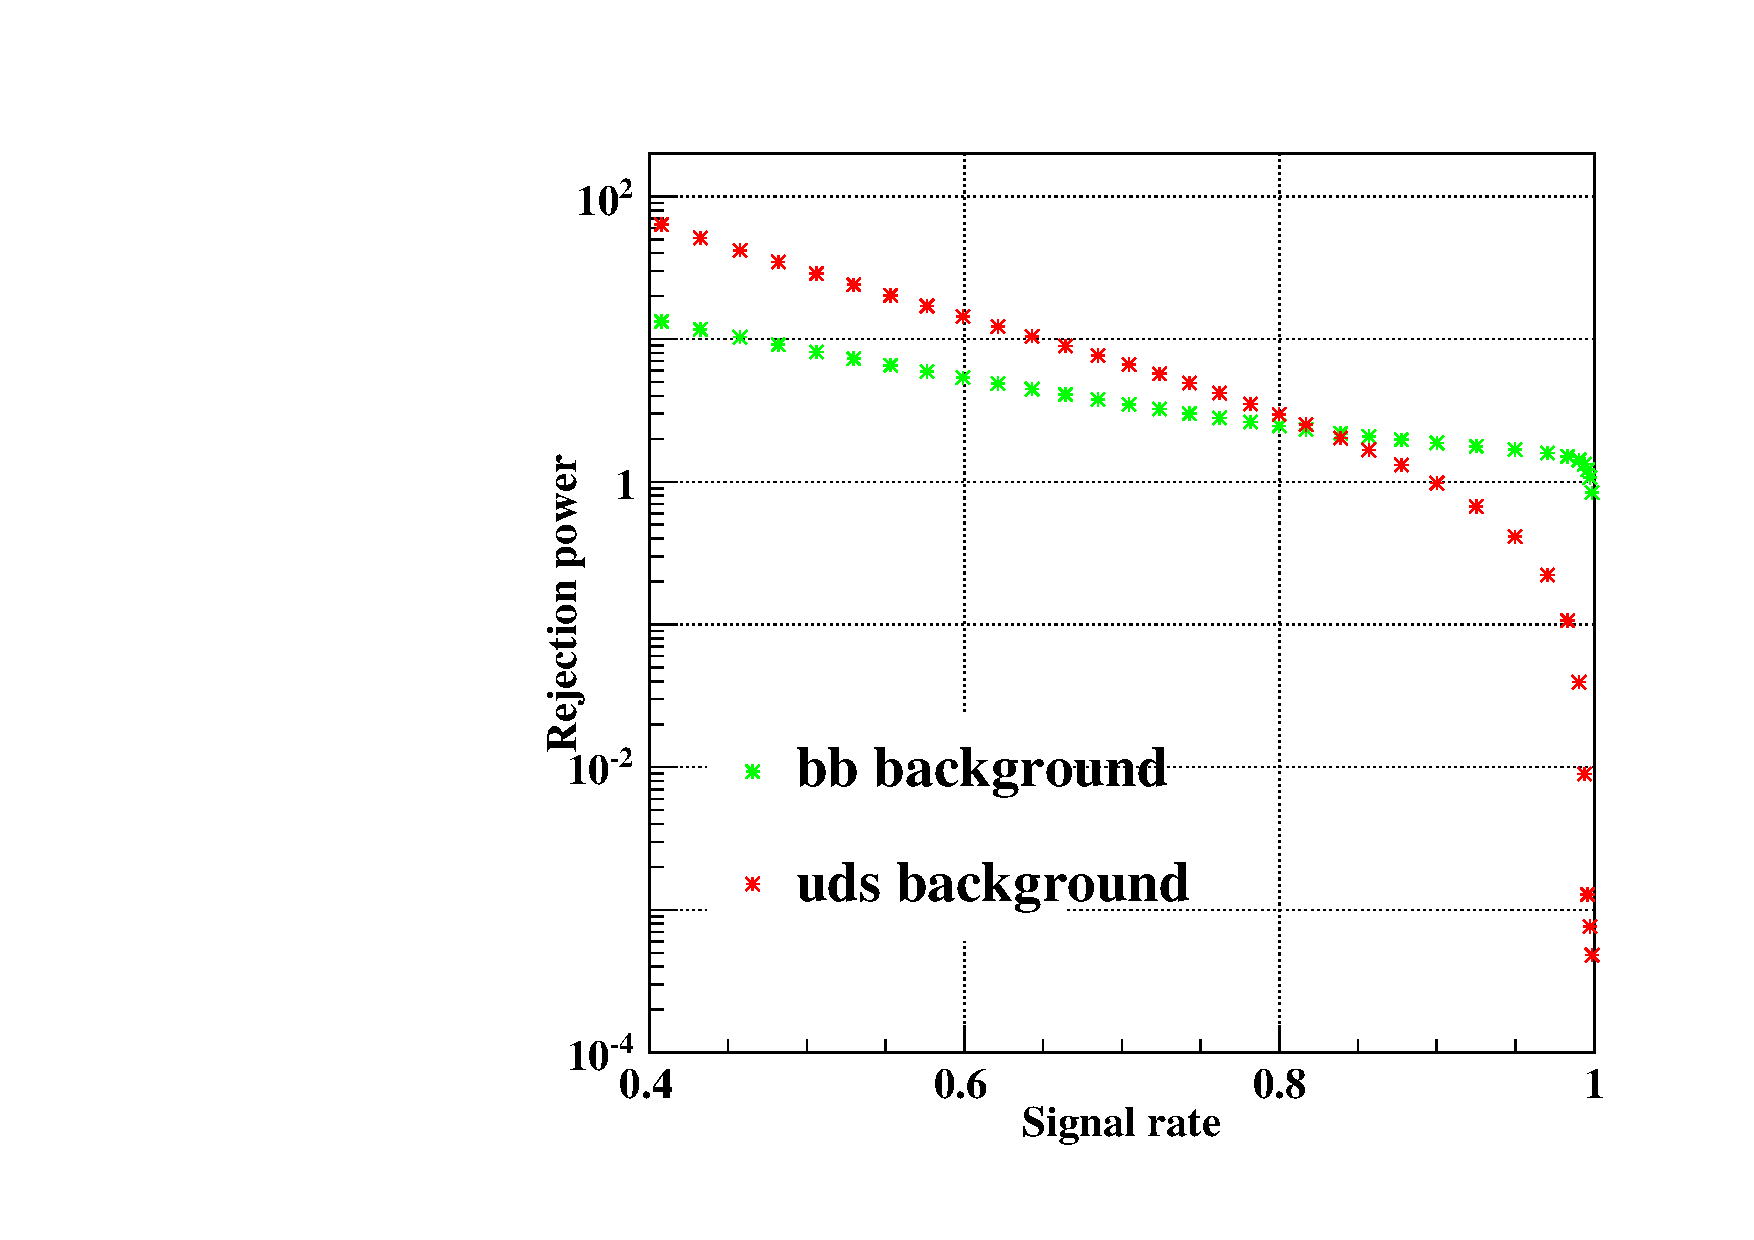
\includegraphics[width=\textwidth]{Btagging/rejectionC-lcfiweights-test.pdf}
    \end{minipage}
}
\caption{Flavor tagging performance curve. Left: b-tagging efficiency as function of rejection against $c$ and light jet. Right: c-tagging efficiency as function of rejetion against $b$ and light jet.}
\end{figure}

 
\subsection{Template fit}\label{subsec:templatefit}
 The b-likenesses of the two jets from higgs decay, say $L_{b1}$ and $L_{b2}$, can be combined to construct a discriminator variable $X_B = \dfrac{L_{b1}L_{b2}}{1-L_{b1}L_{b2}}$.  The conservation of quark flavor in higgs decay guarantee that $X_B$ is close to 1 if higgs decay to $b\bar{b}$ while close to 0 in other case. 
 Similar variable are defined for c-likeness: $X_C = \dfrac{L_{c1}L_{c2}}{1-L_{c1}L_{c2}}$. A set of template is defined according to the signal and background's $X_B-X_C$ distribution.  The distribution of template for $H\to gg/bb/cc$ is shown in figure \ref{fig:sig_template}. These distributions are 
 defined as flavor PDFs in the fit. For the dominant background like semi-leptonic $ZZ$ events and $ZH\to \llh$ background, there are also such flavor templates defined as flavor PDFs.\par
% The $X_B-X_C$ distribution in 'data', which is composed from signal and background simulation events, is shown in figure \ref{fig:data_template}.
% \begin{figure}[!htpb]
% \label{fig:data_template}
% \centering
% \subfigure[]
%{
%  \begin{minipage}[b]{0.42\textwidth}
%  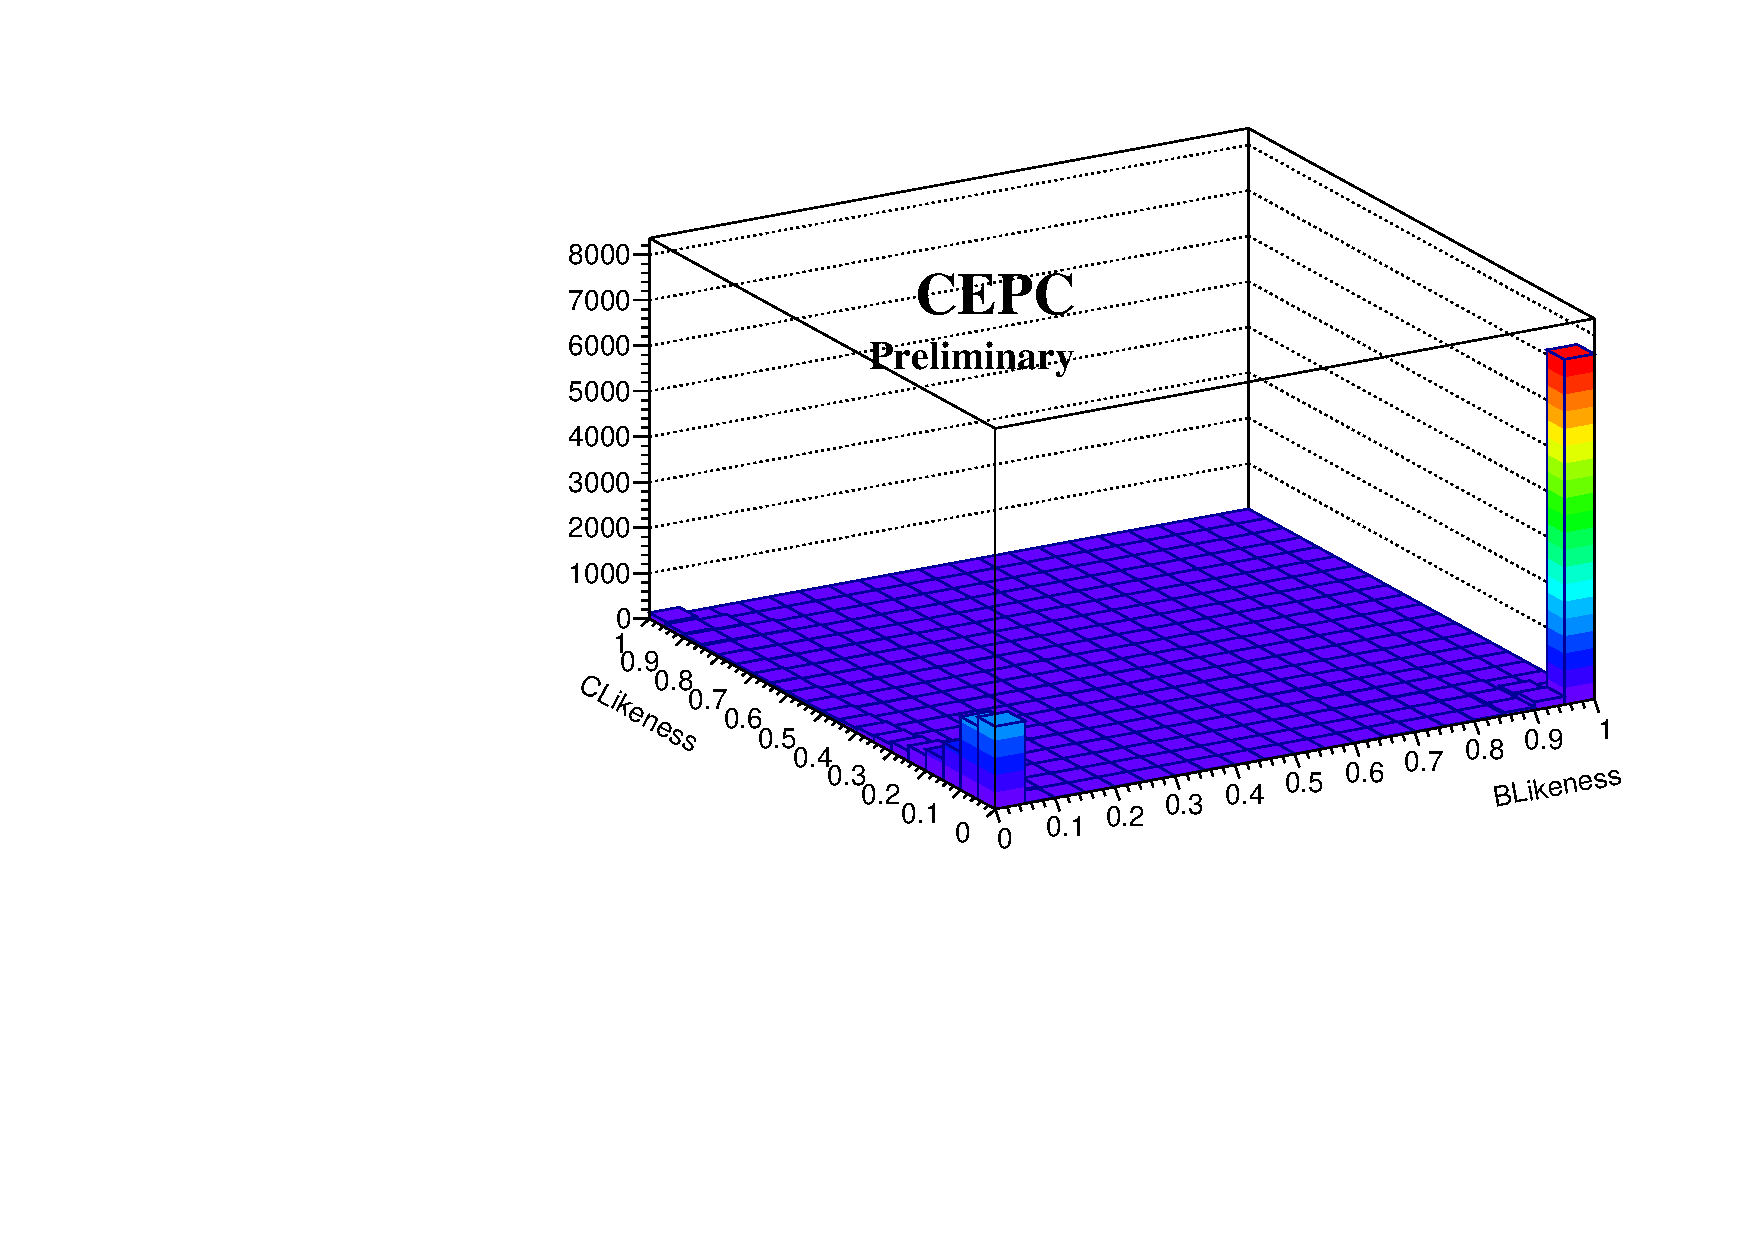
\includegraphics[width=\textwidth]{Template/eeh_data.pdf}
%  \end{minipage}
%}
%\subfigure[]
%{
%  \begin{minipage}[b]{0.42\textwidth}
%  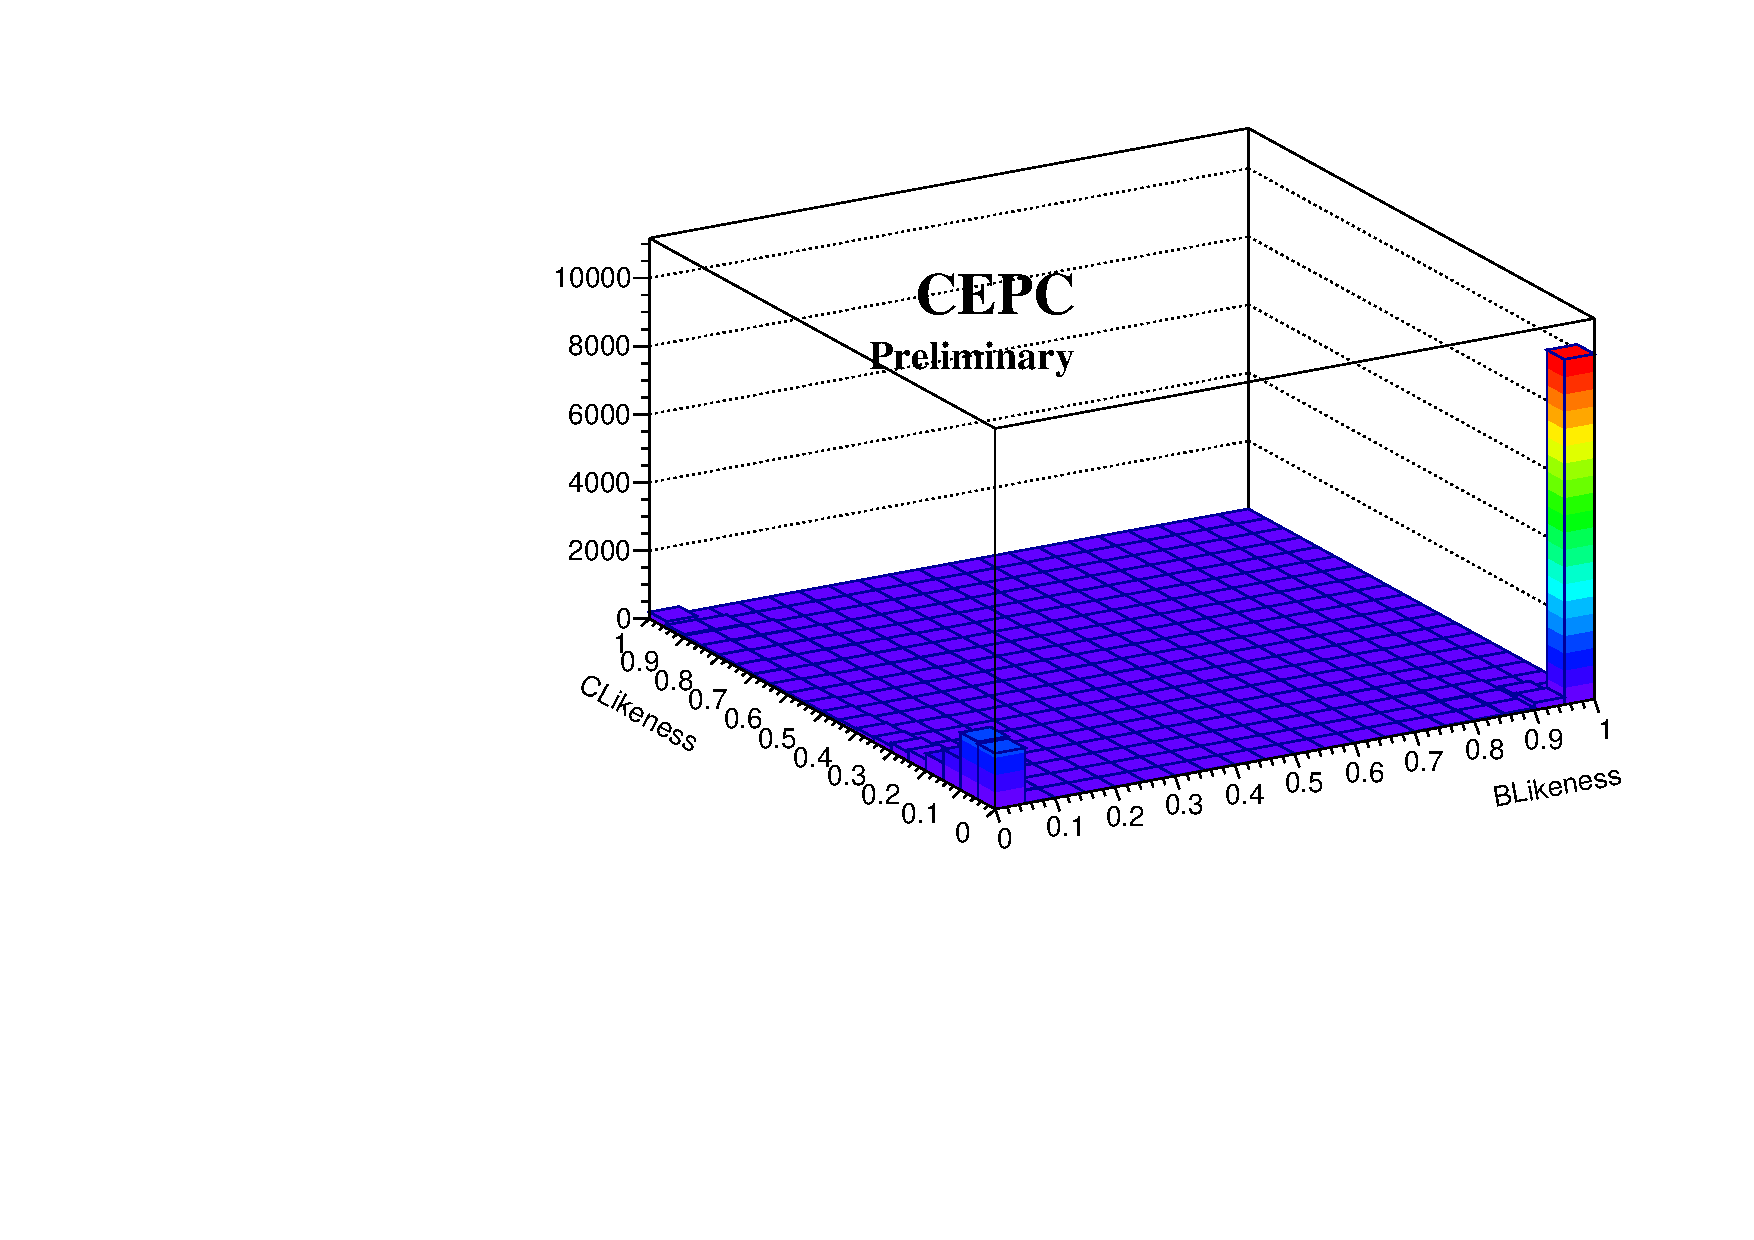
\includegraphics[width=\textwidth]{Template/mumuh_data.pdf}
%  \end{minipage}
%}
%%\subfigure[]
%%{ 
%%   \begin{minipage}[b]{0.42\textwidth}
%%   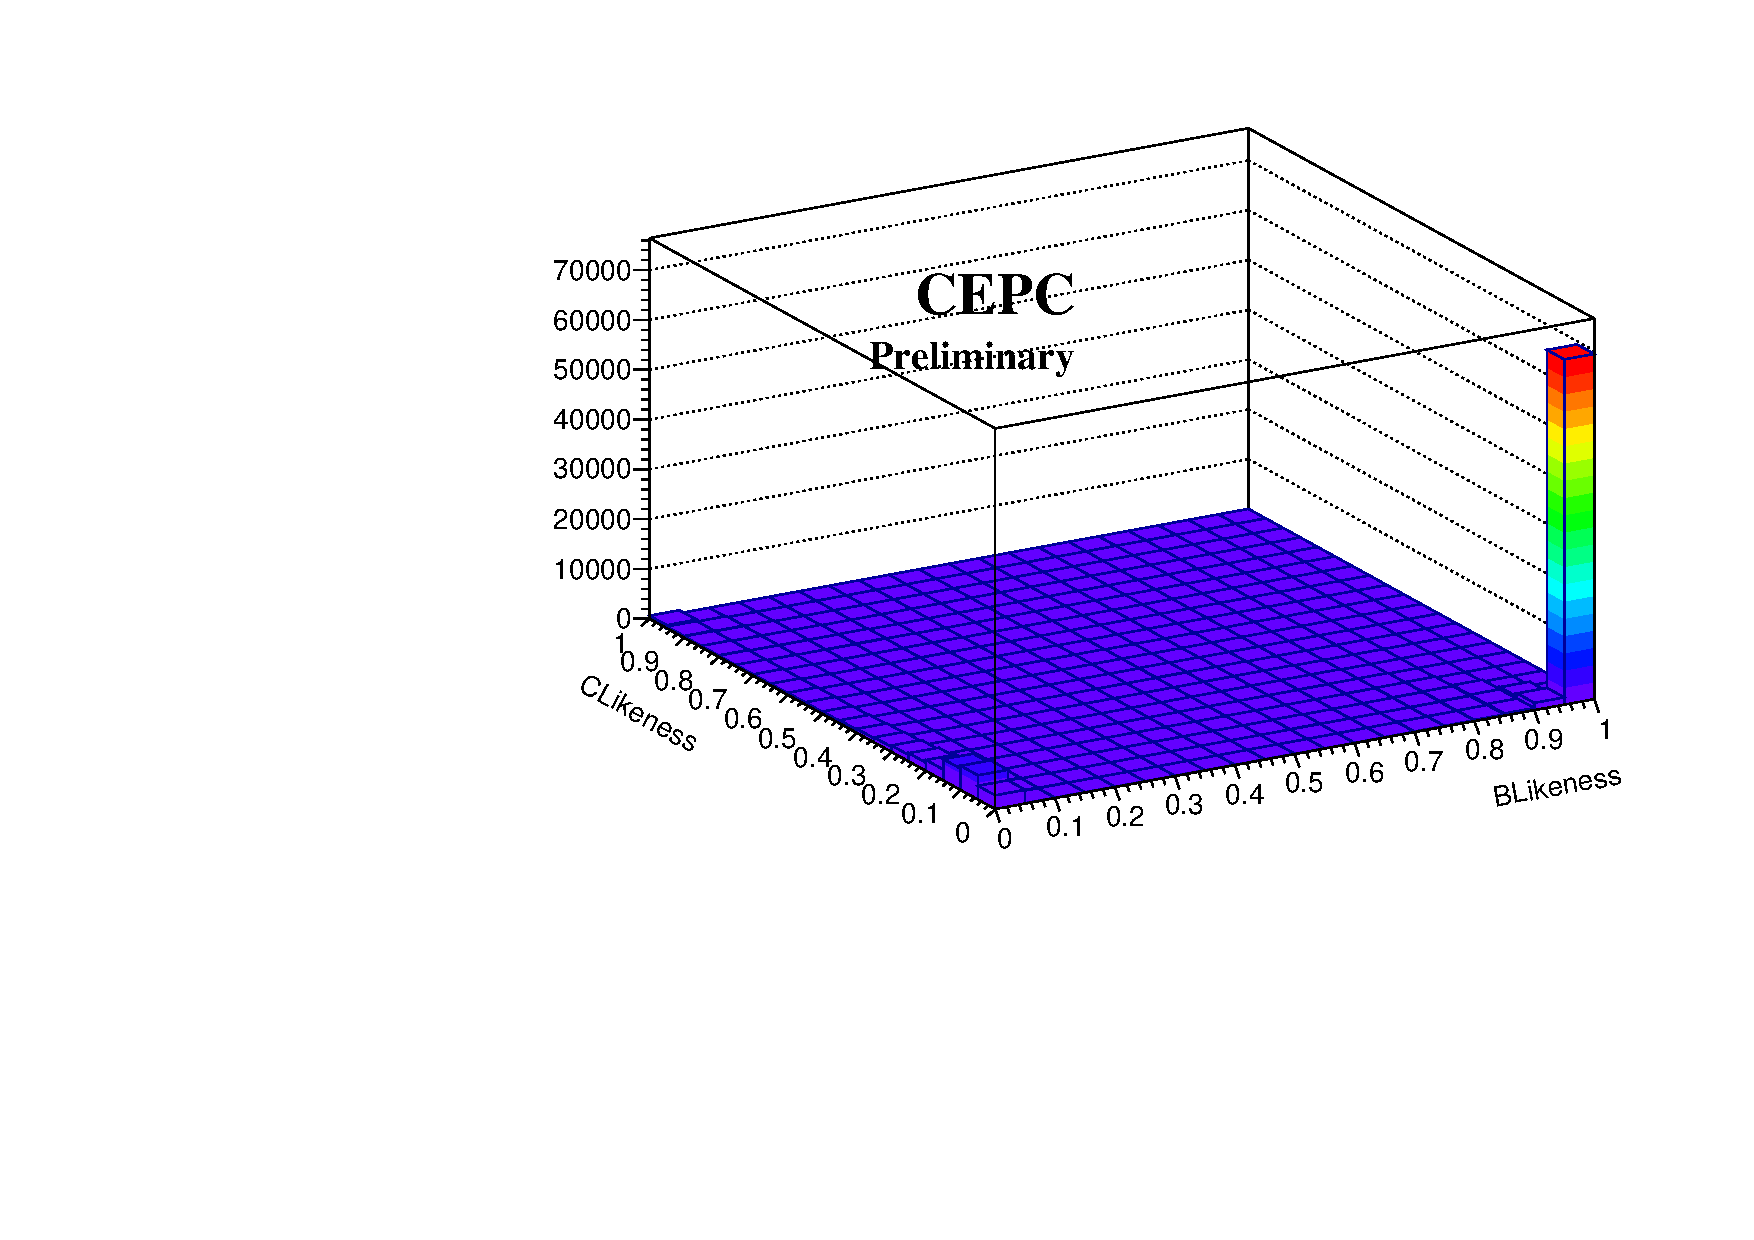
\includegraphics[width=\textwidth]{Template/nnh_data.pdf}
%%   \end{minipage}
%%}
%%\subfigure[]
%%{
%%    \begin{minipage}[b]{0.42\textwidth}
%%    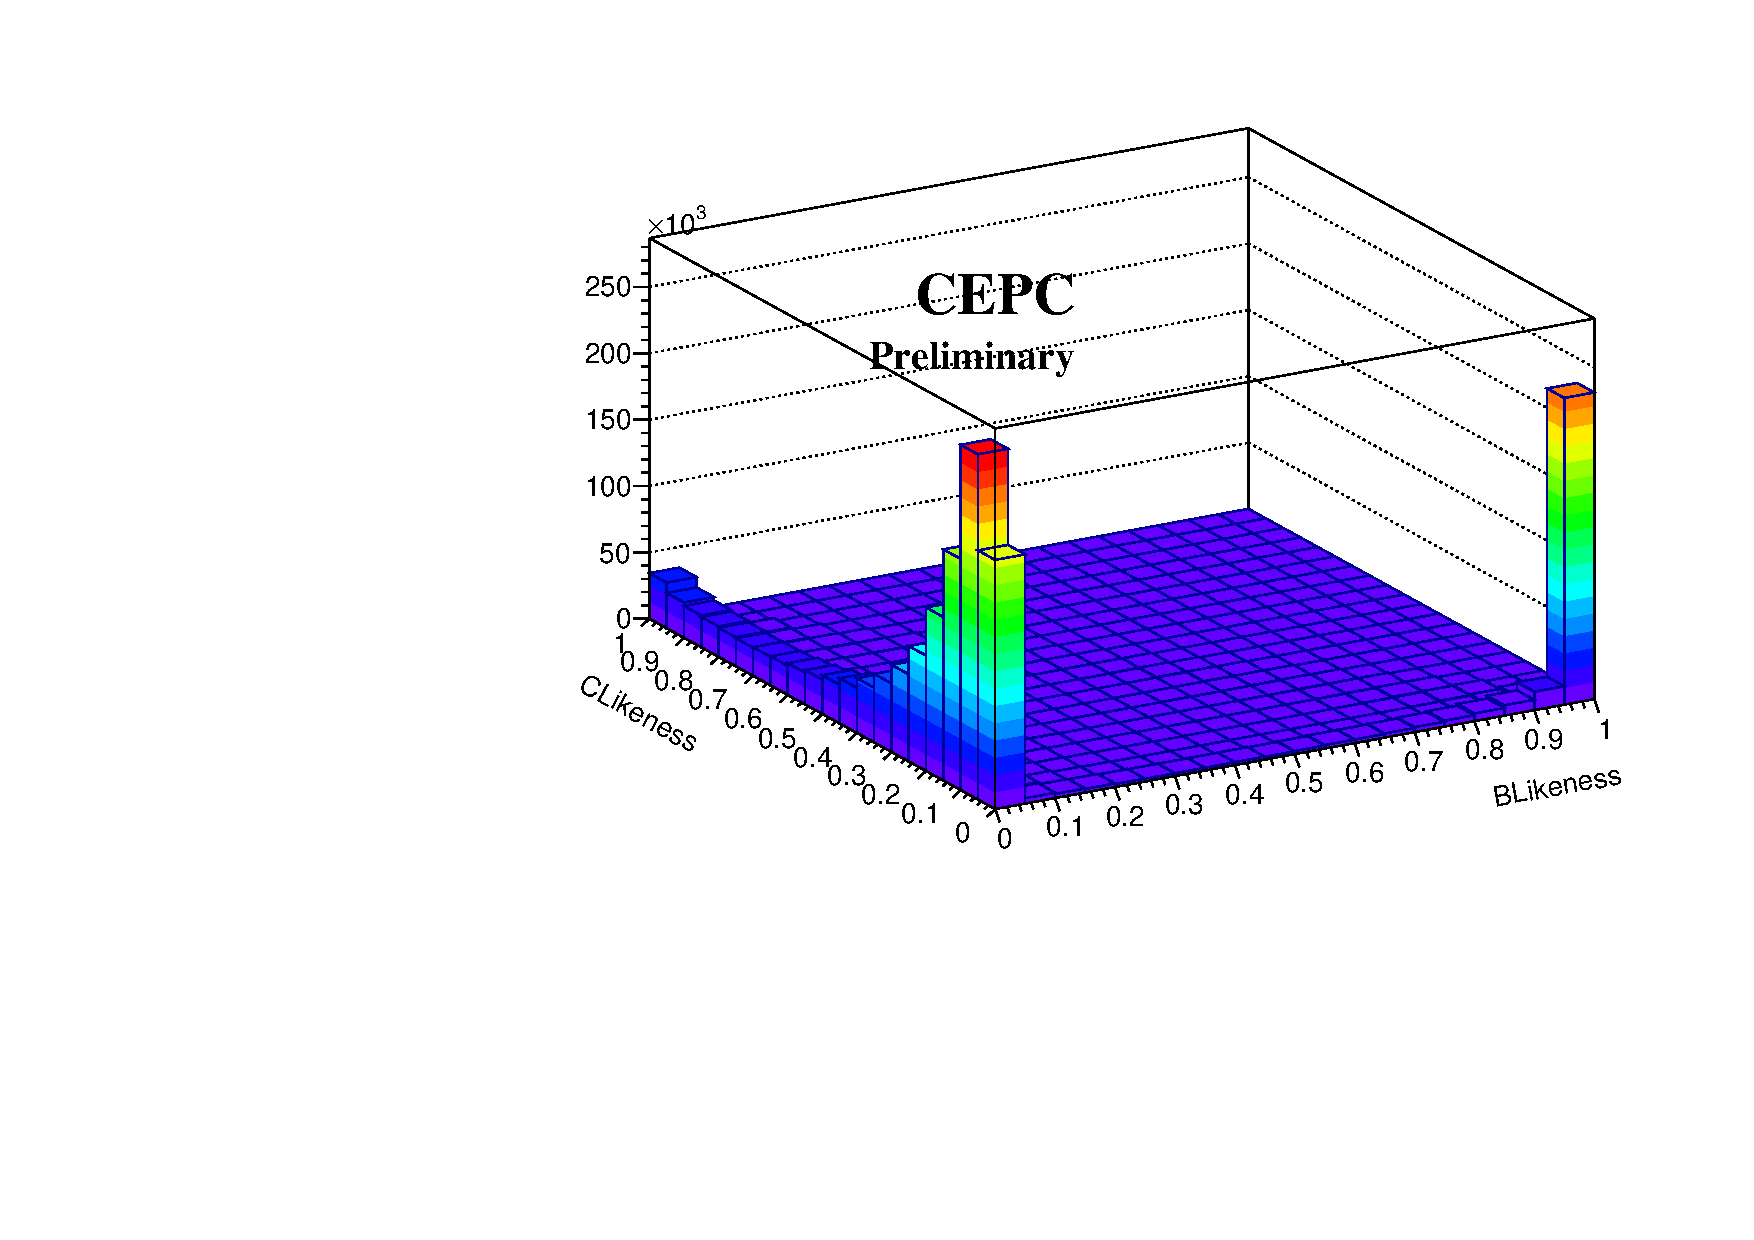
\includegraphics[width=\textwidth]{Template/qqh_data.pdf}
%%    \end{minipage}
%%}
% \caption{$X_B-X_C$ distribution of pesudo-data in each channel: templates of \eeh(top left),\mmh(top right),\nnh(bottom left) and \qqh(bottom right)}
% \end{figure}

% A likelihood was constructed according to the template distribution:
% \begin{equation}
% \log{L} = \sum\limits_{i=1}^N{\log{Possion(\mu_{i},n_{i})}}
% \label{for:template}
% \end{equation}
%in which i is the bin index(we have 20 bins for $X_B$ and $X_C$ so in all $N=400$); $Possion(\mu_{i},n_{i})$ is the Possion likelihood with for $n_{i}$ obvserved event and expectation $\mu_{i}$, which include the parameter of interest:
%\begin{equation}
%\mu_{i} = \sum\limits_{j=1}^s f_j\times\mu_{i,j}
%\end{equation}
%in which j is the index of templates (one template for each components); $f_j$ is the fraction of $j$th components which need to be worked out; $\mu_{i,j}$ stands for the expected event yields of $j$th components in $i$th bin. Minimize $-\log{L}$ we can fit the $f_j$. The distribution of template for $H\to gg/bb/cc$ is shown in figure \ref{fig:sig_template}. The $\Hboson \to \bpair$ and $\Hboson \to\cpair$ concentrate in region (1,0) and (0,1) respectively, while $\Hboson\to\gpair$ tends to distribute around (0,0). It can be found a tail at (1,0) show up in $\Hboson$ distribution, which are due to contribution of gluon splitting $g\to \bpair$(\eeh,\mmh and \nnh) and hadronic $Z-$decay(\qqh).
 
\begin{figure}[!htpb]
\label{fig:sig_template}
\centering
%\subfigure[]
%{
%  \begin{minipage}[b]{0.31\textwidth}
%  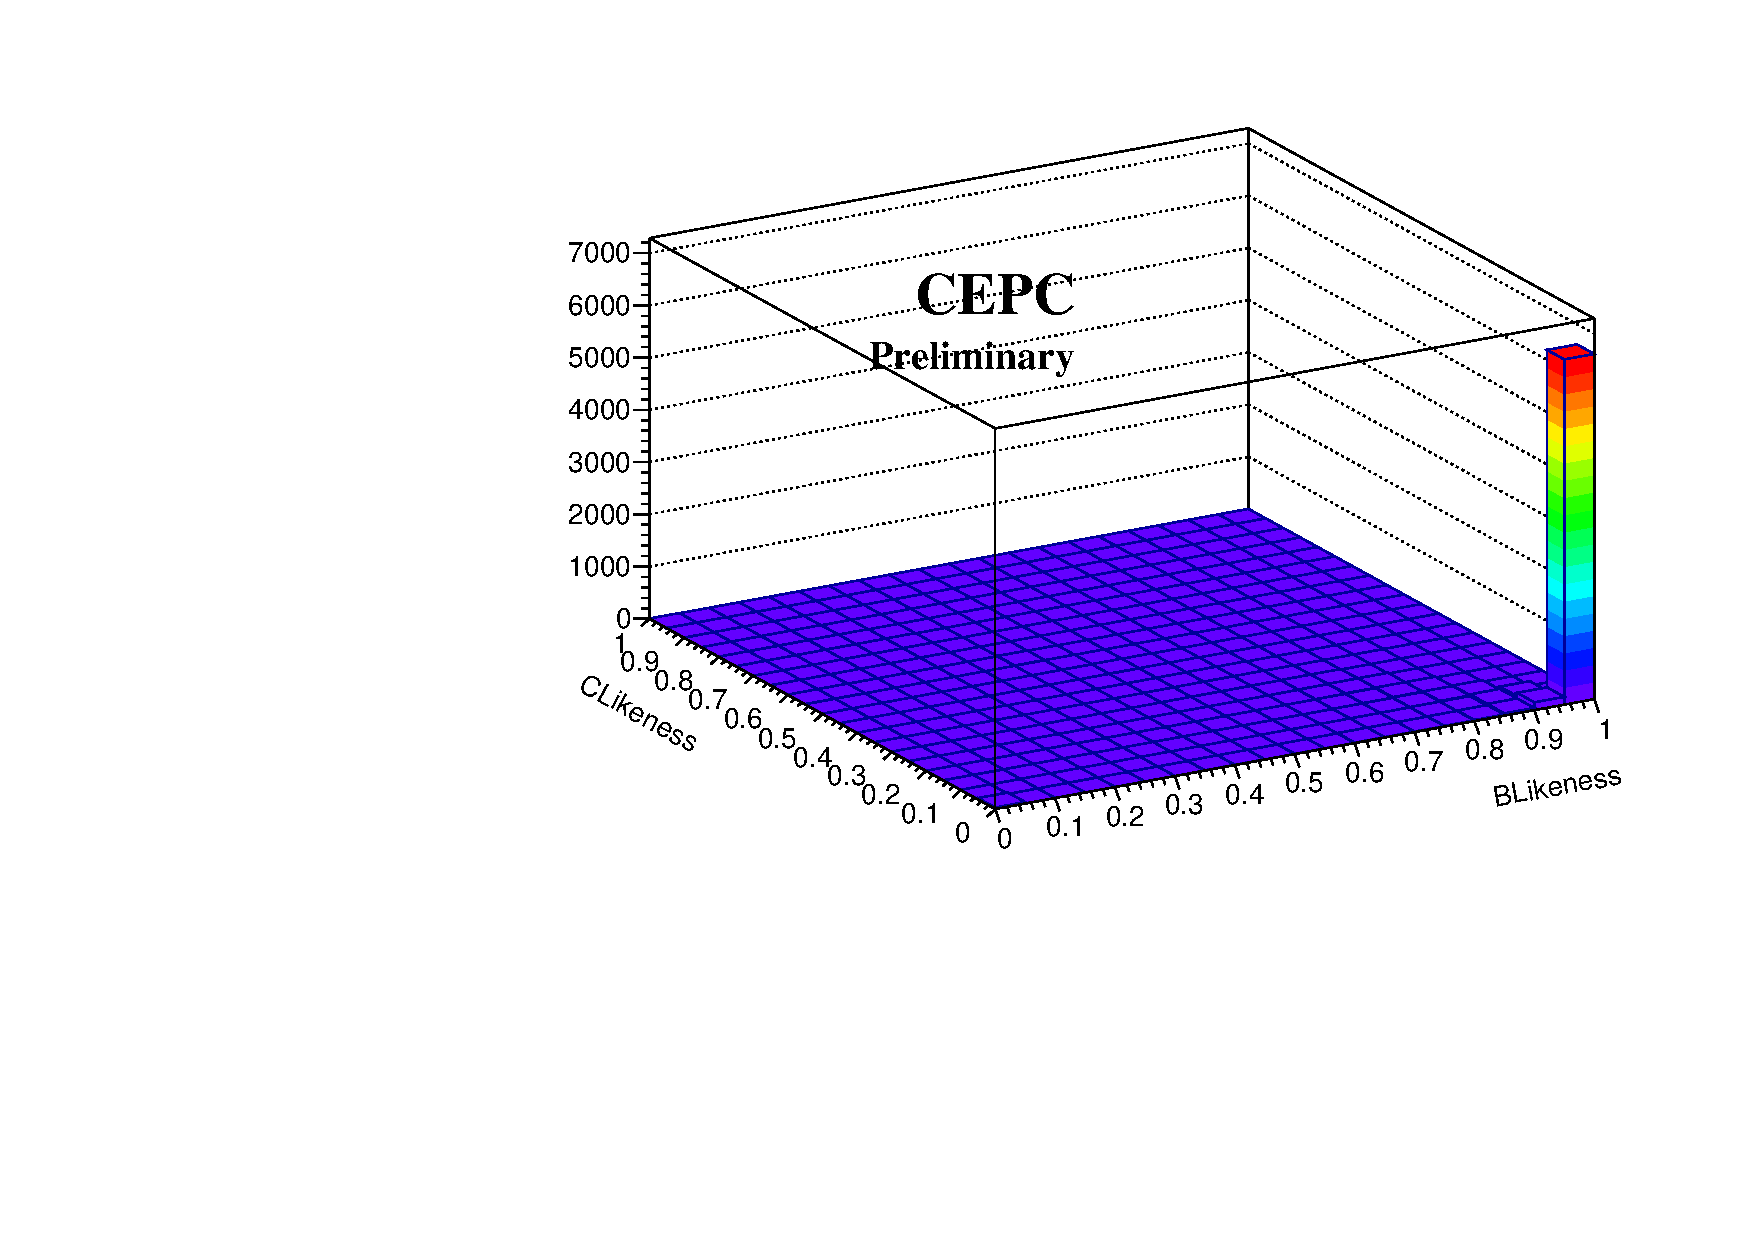
\includegraphics[width=\textwidth]{Template/eeh_bb.pdf}
%  \end{minipage}
%}
%\subfigure[]
%{
%  \begin{minipage}[b]{0.31\textwidth}
%  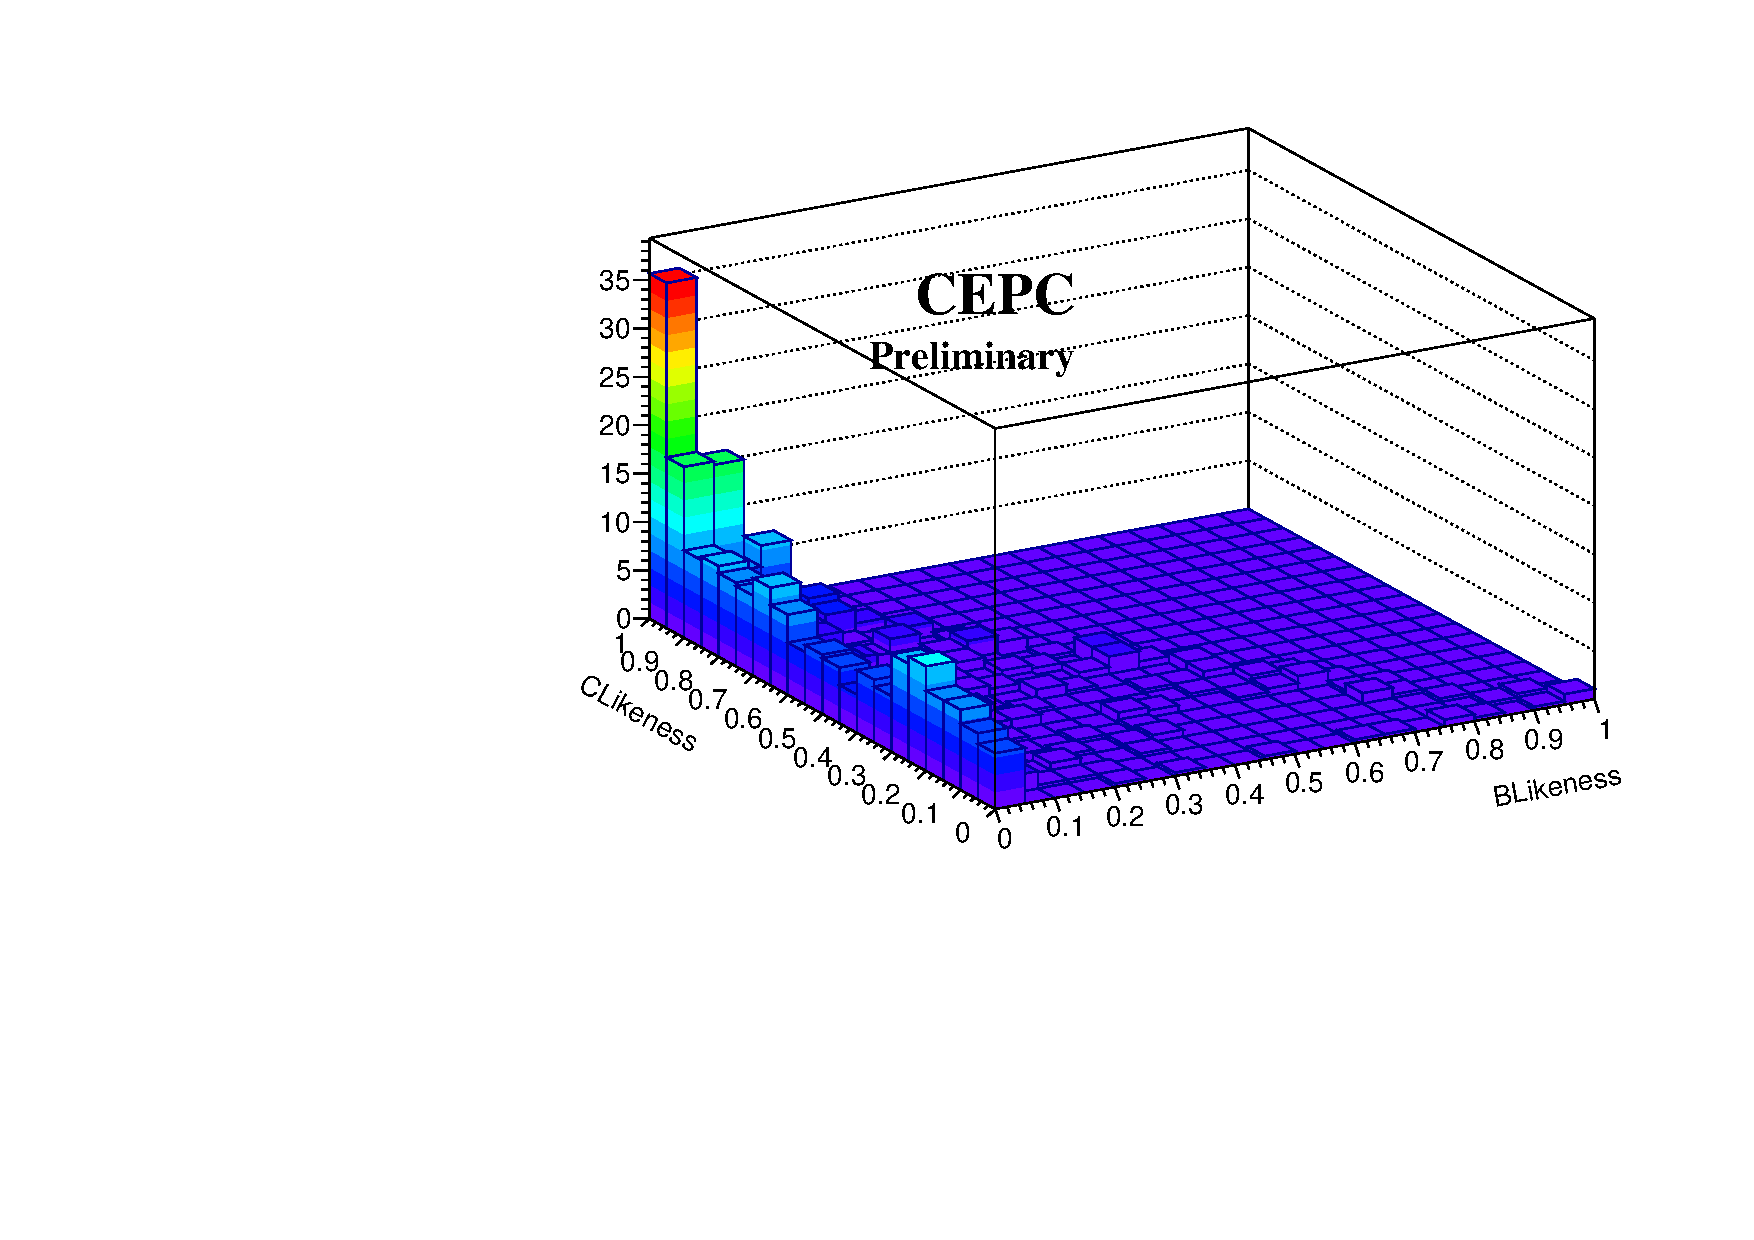
\includegraphics[width=\textwidth]{Template/eeh_cc.pdf}
%  \end{minipage}
%}
%\subfigure[]
%{ 
%   \begin{minipage}[b]{0.31\textwidth}
%   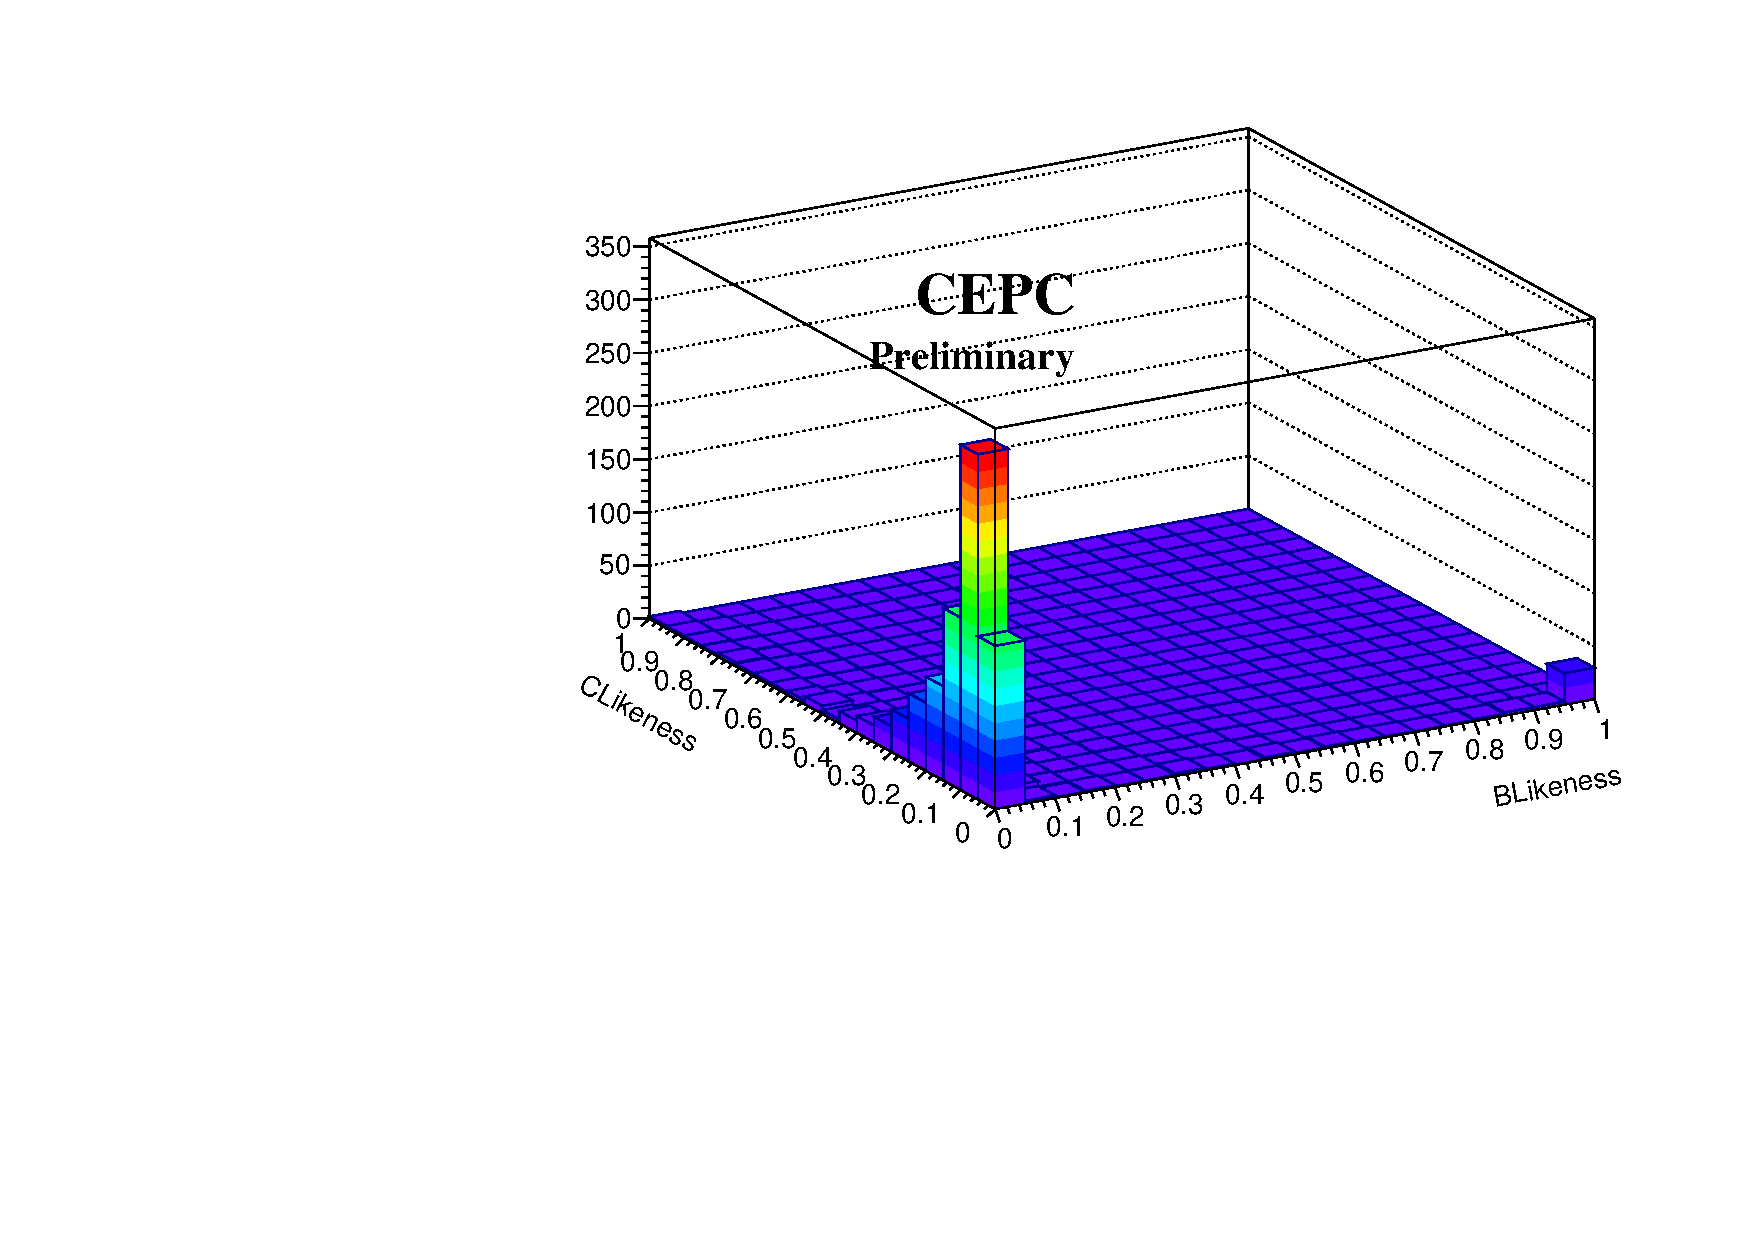
\includegraphics[width=\textwidth]{Template/eeh_gg.pdf}
%   \end{minipage}
%}
\subfigure[]
{
    \begin{minipage}[b]{0.31\textwidth}
    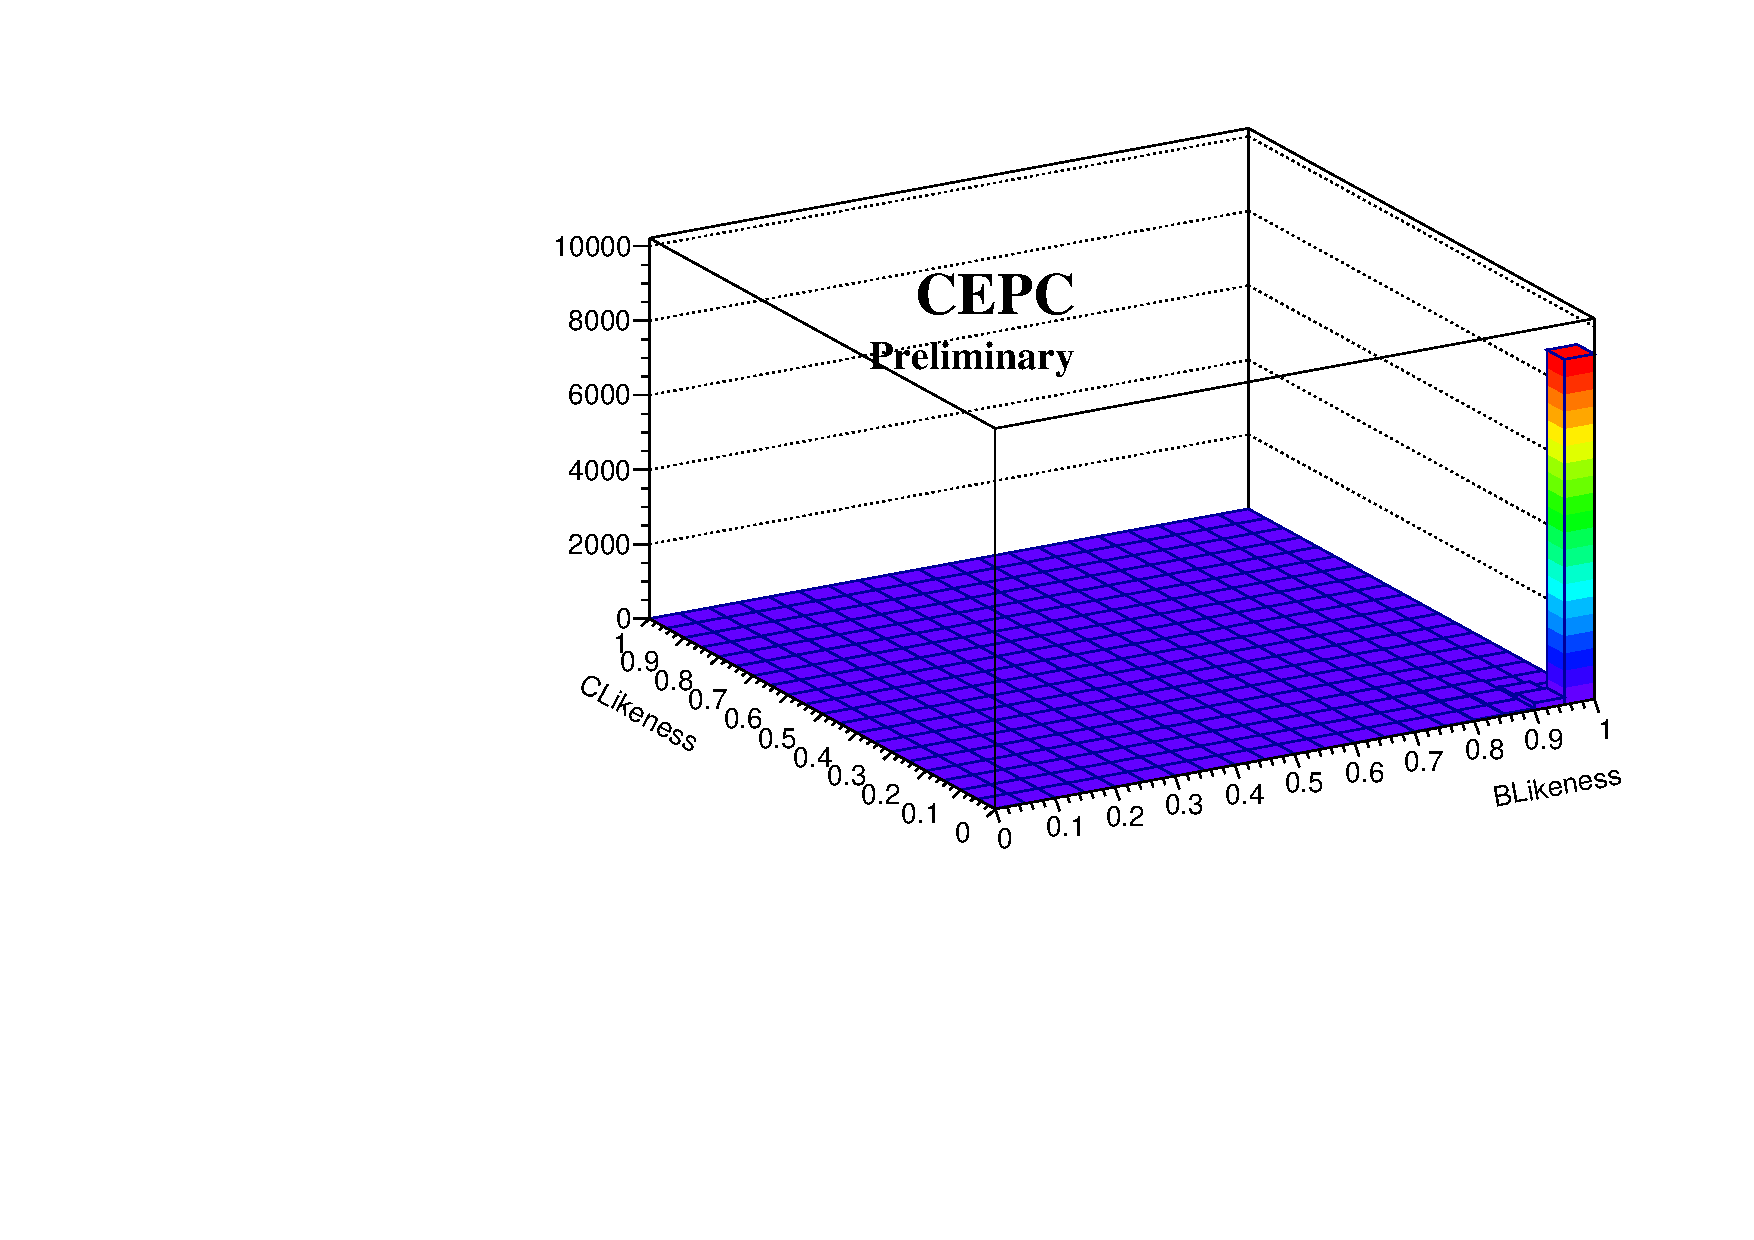
\includegraphics[width=\textwidth]{Template/mumuh_bb.pdf}
    \end{minipage}
}
\subfigure[]
{ 
   \begin{minipage}[b]{0.31\textwidth}
   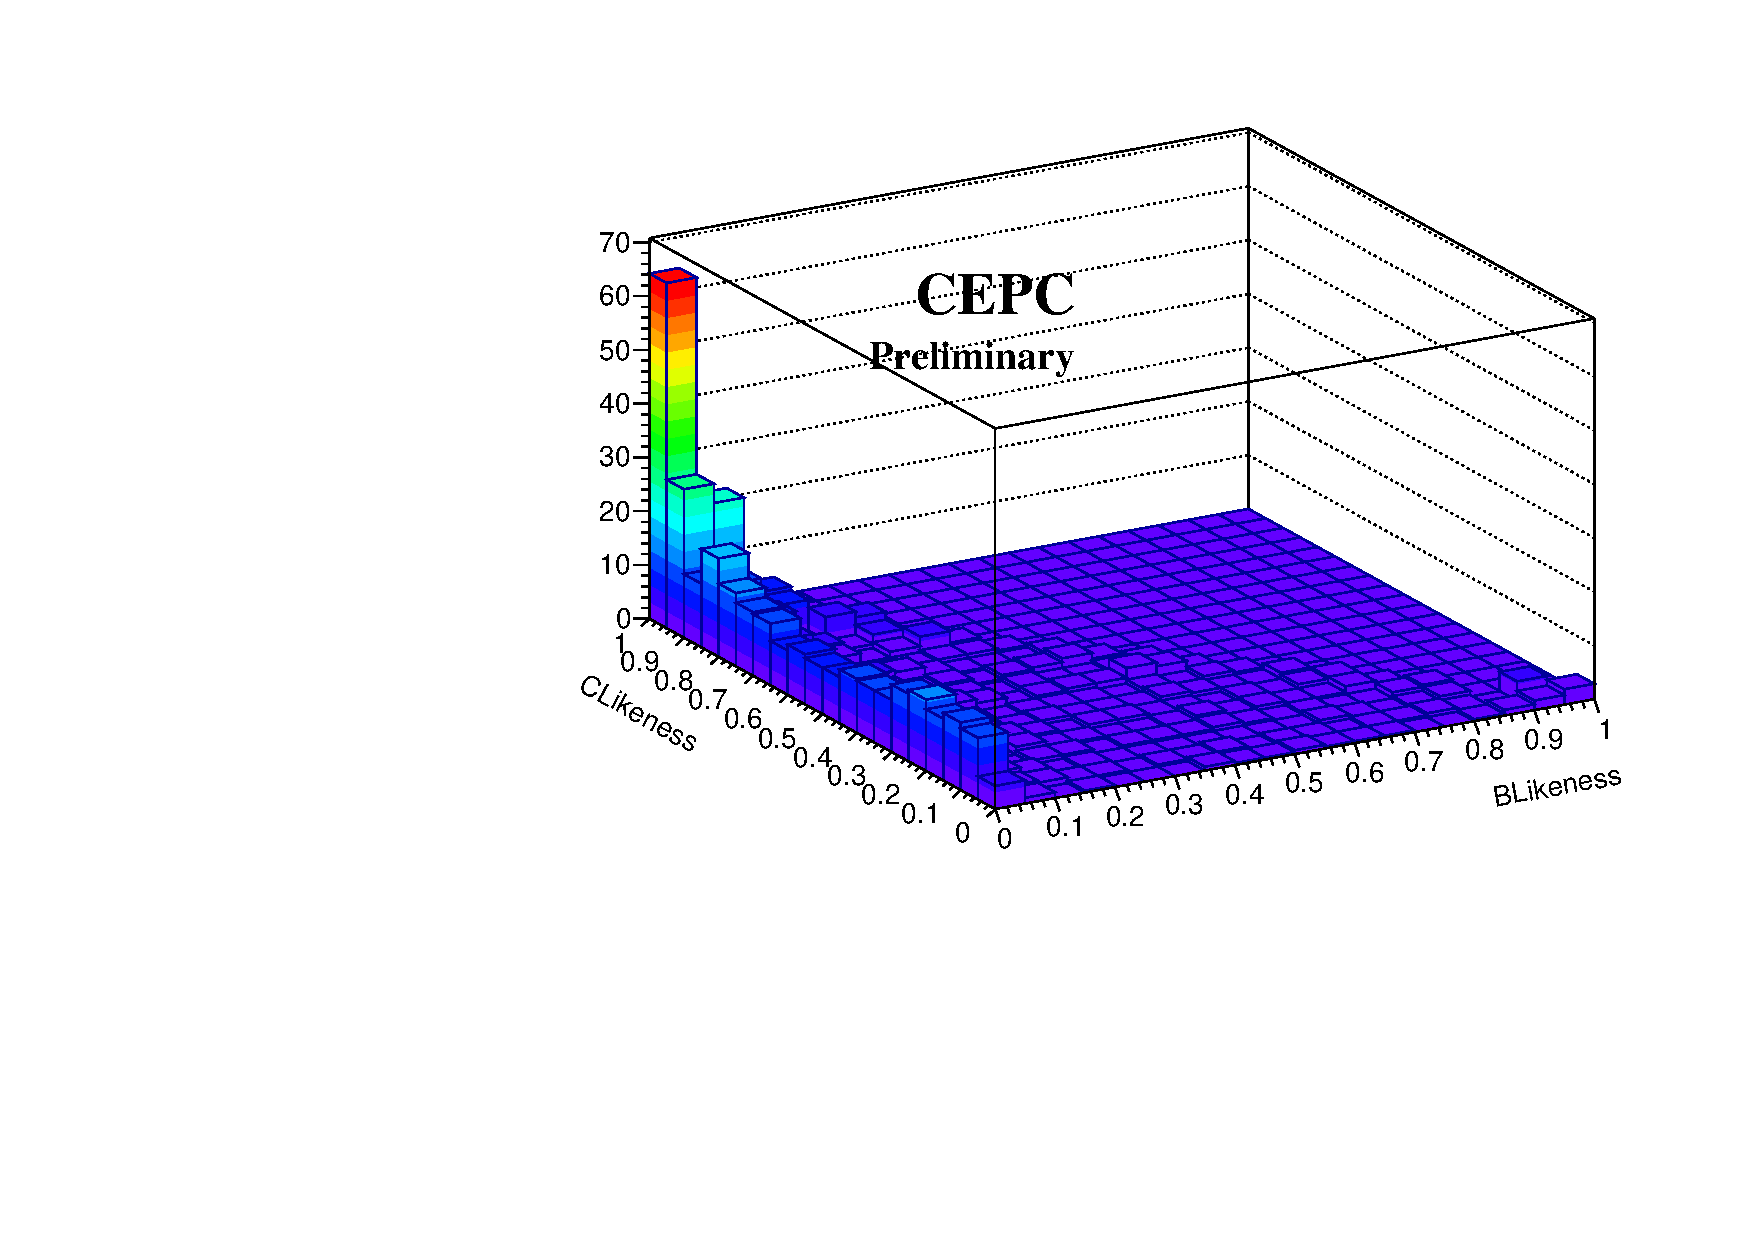
\includegraphics[width=\textwidth]{Template/mumuh_cc.pdf}
   \end{minipage}
}
\subfigure[]
{
    \begin{minipage}[b]{0.31\textwidth}
    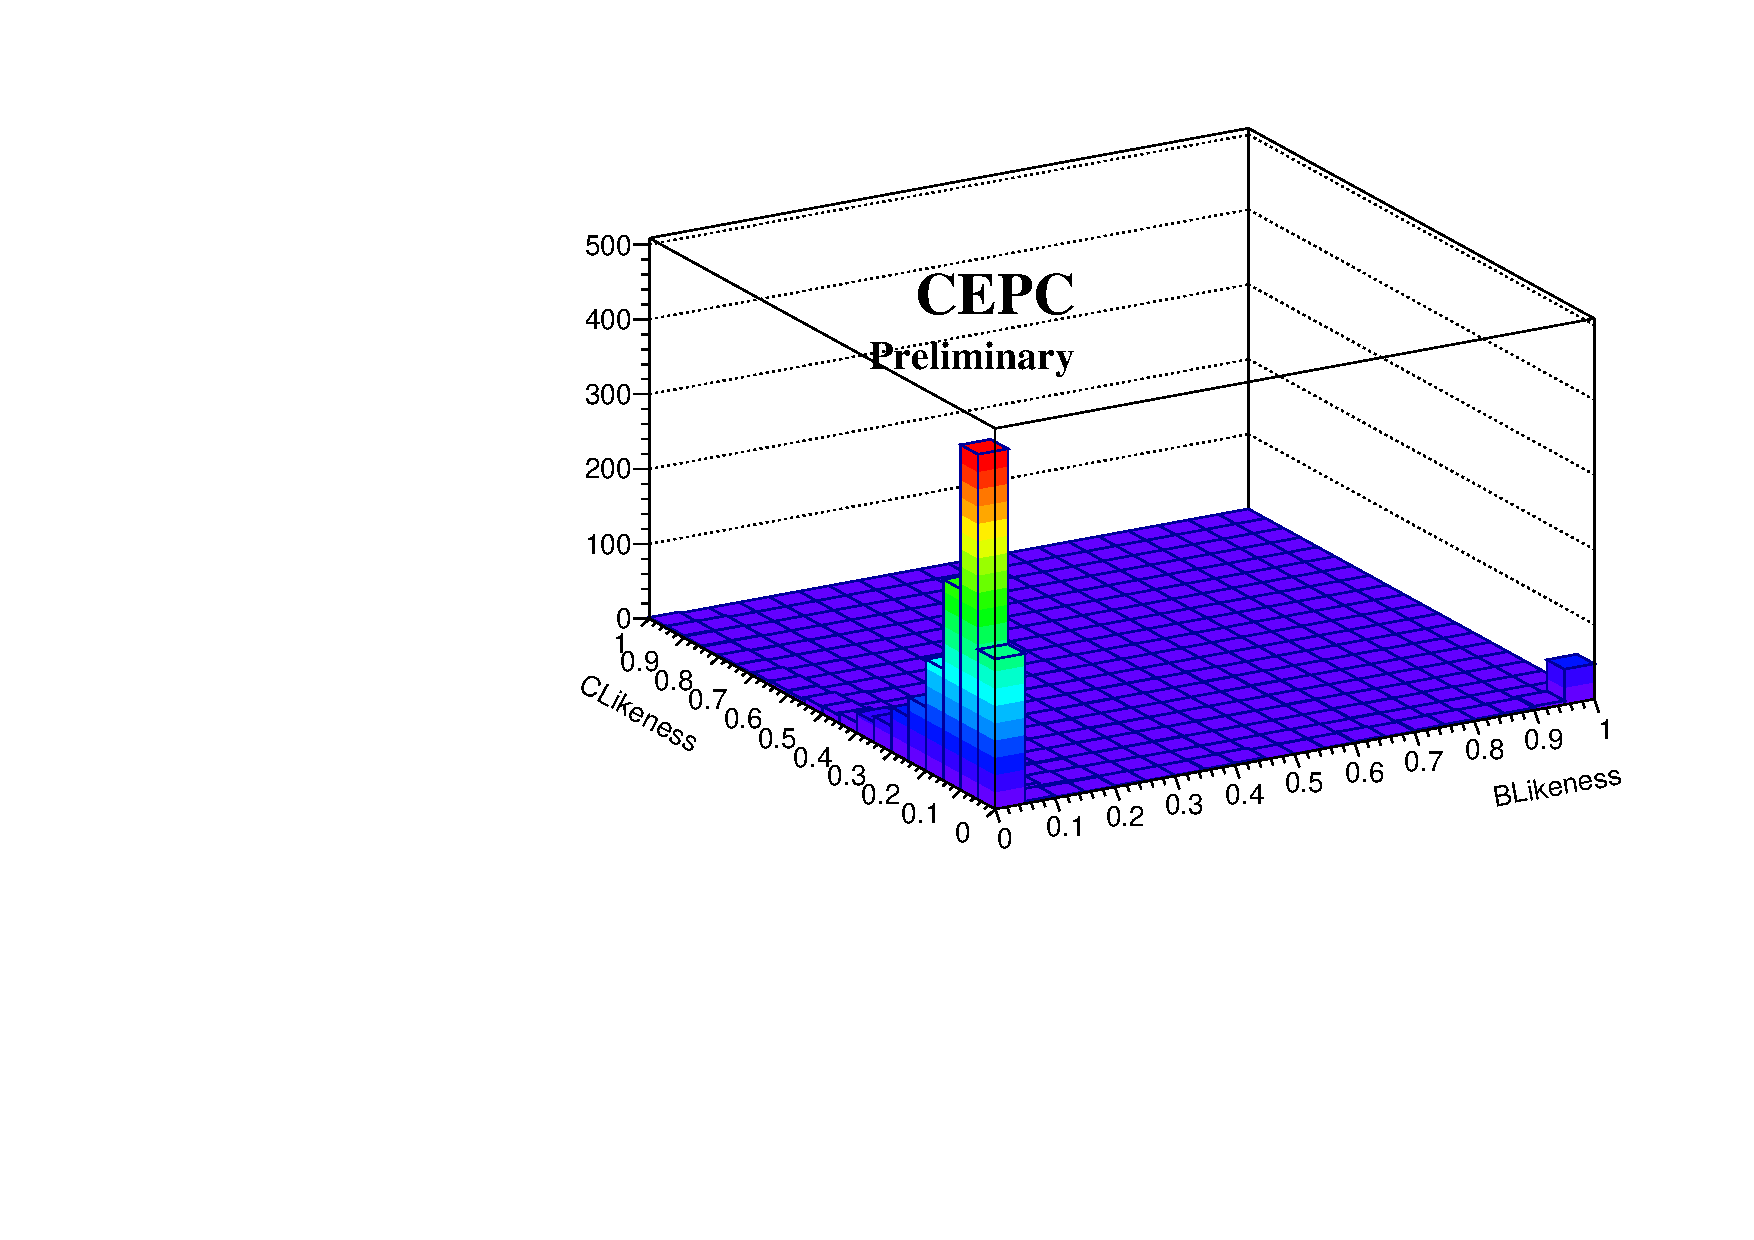
\includegraphics[width=\textwidth]{Template/mumuh_gg.pdf}
    \end{minipage}
}
%\subfigure[]
%{
%    \begin{minipage}[b]{0.31\textwidth}
%    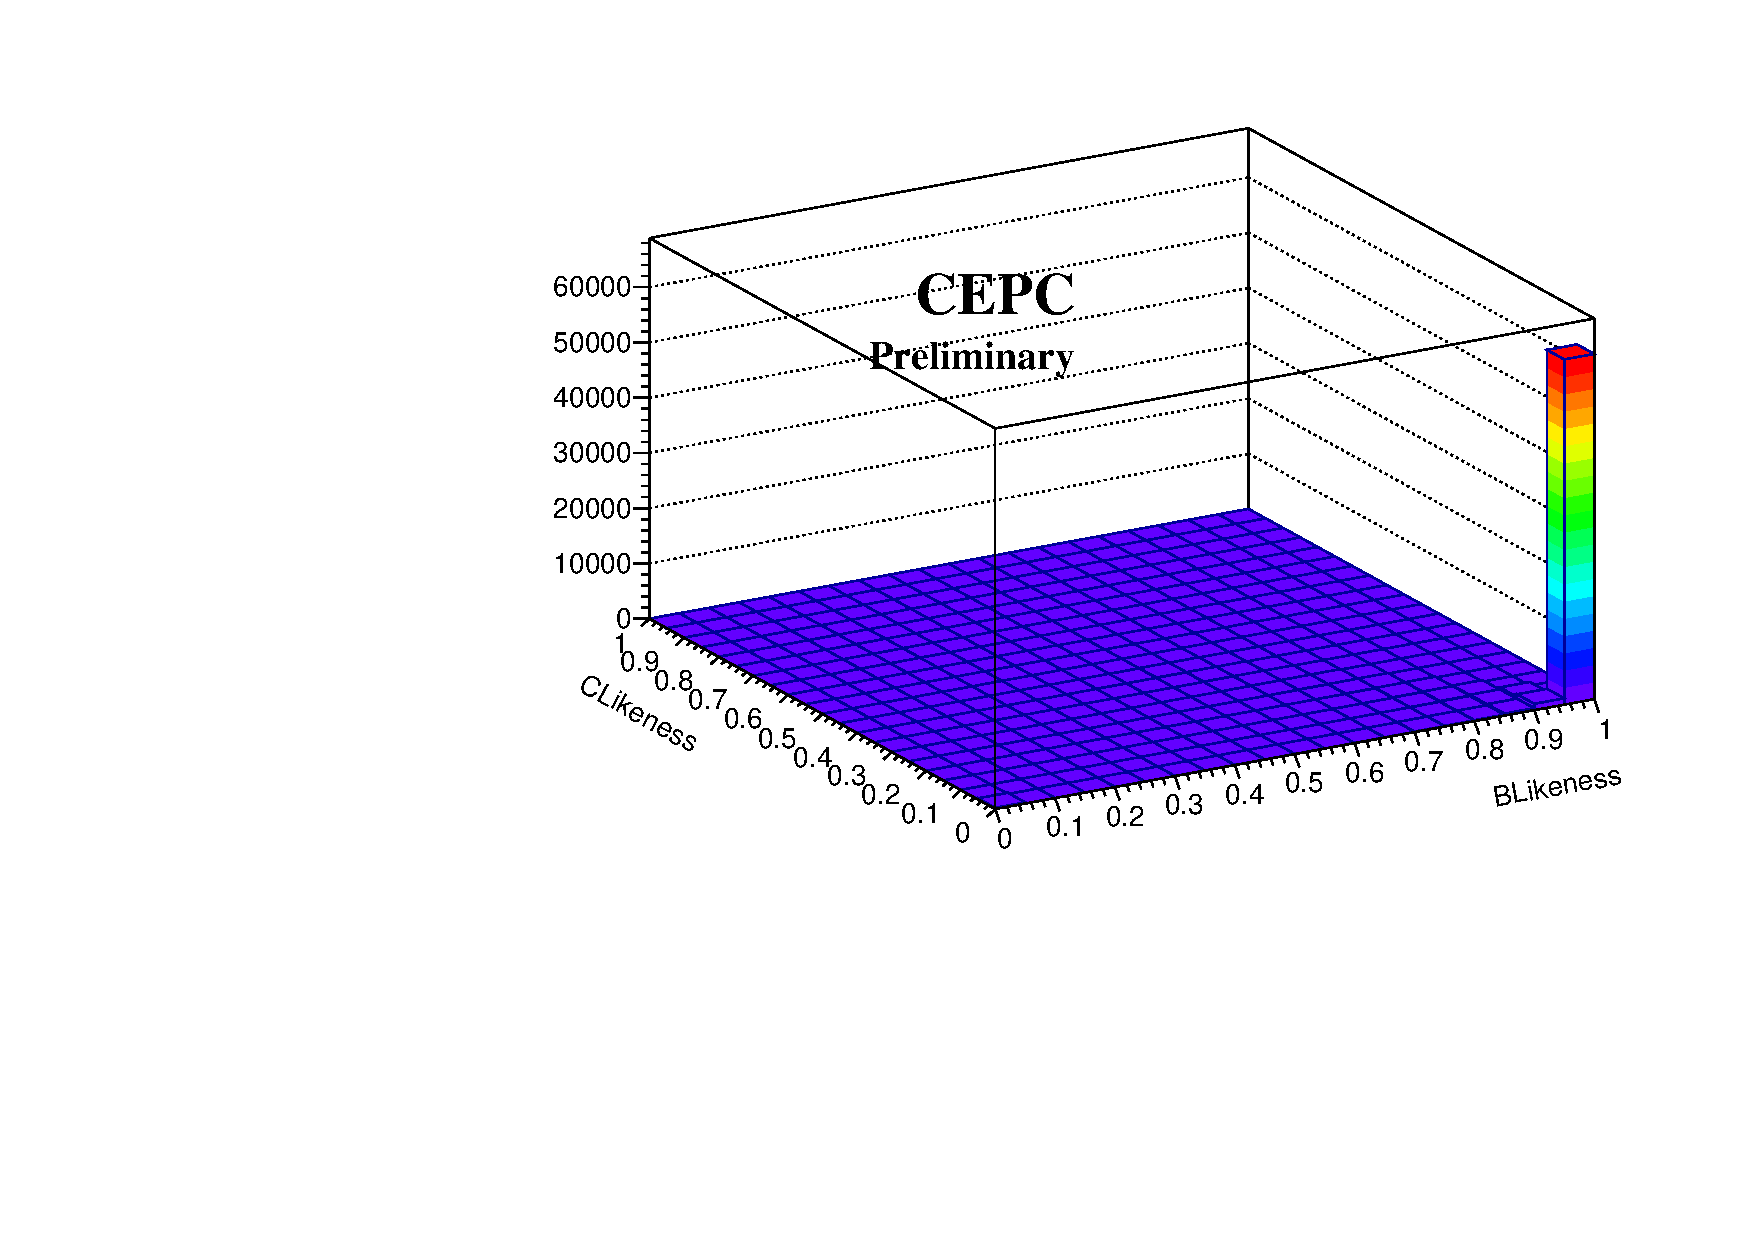
\includegraphics[width=\textwidth]{Template/nnh_bb.pdf}
%    \end{minipage}
%}
%\subfigure[]
%{ 
%   \begin{minipage}[b]{0.31\textwidth}
%   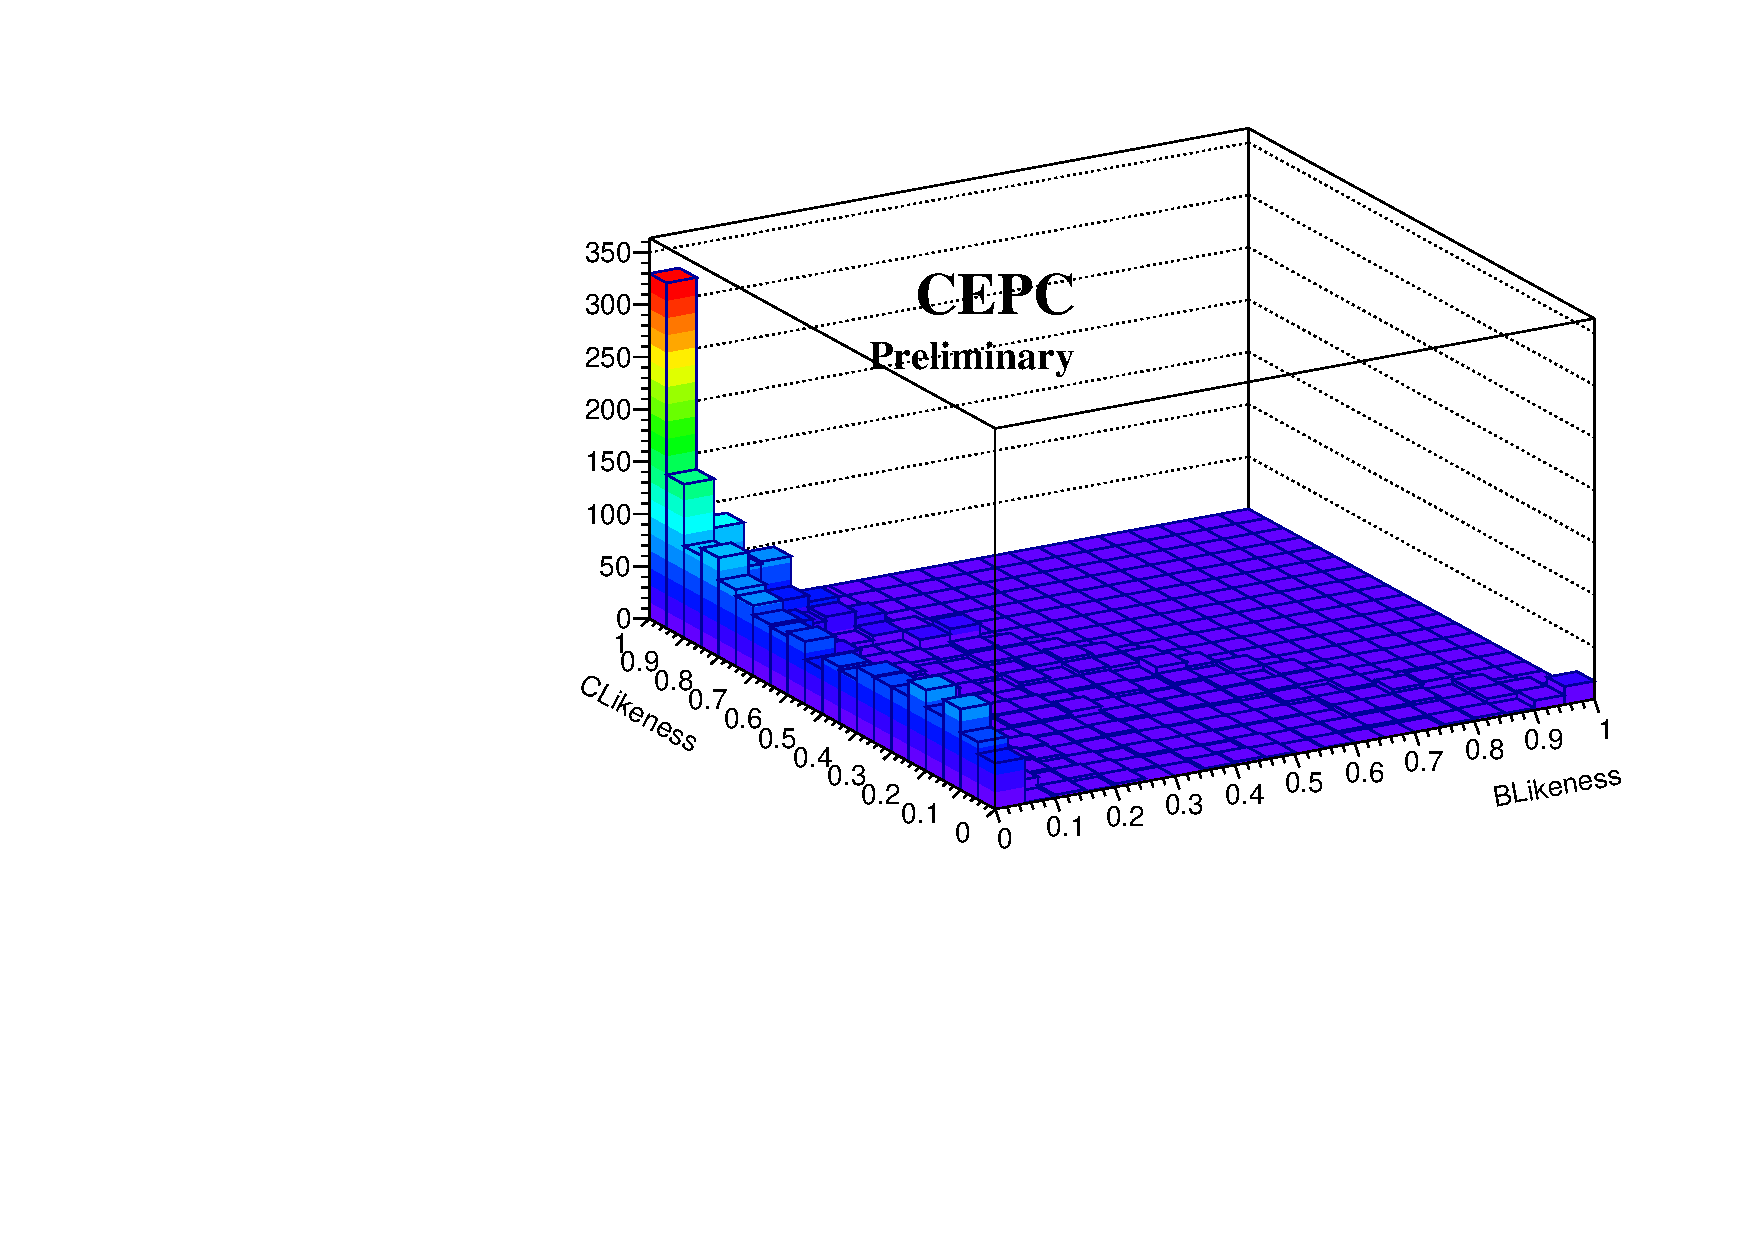
\includegraphics[width=\textwidth]{Template/nnh_cc.pdf}
%   \end{minipage}
%}
%\subfigure[]
%{
%    \begin{minipage}[b]{0.31\textwidth}
%    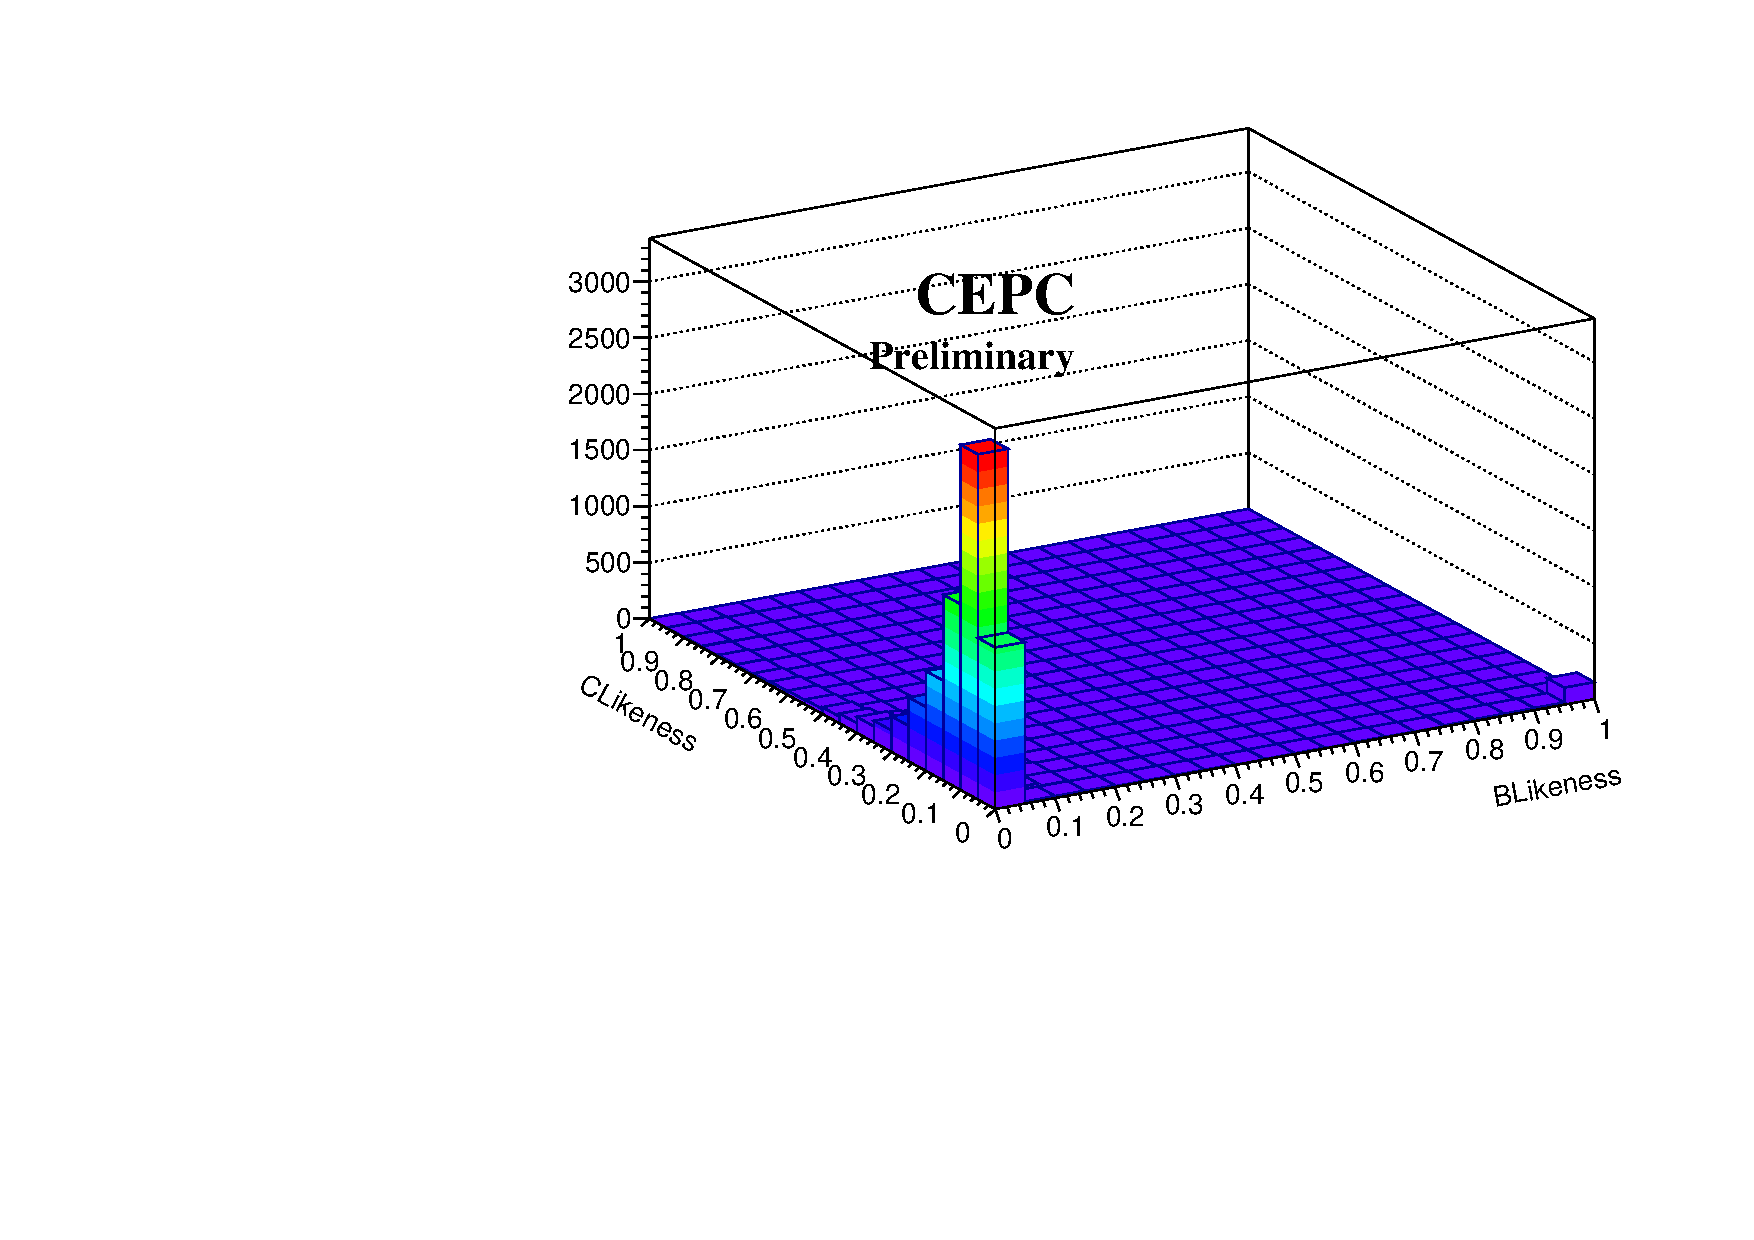
\includegraphics[width=\textwidth]{Template/nnh_gg.pdf}
%    \end{minipage}
%}
%\subfigure[]
%{
%    \begin{minipage}[b]{0.31\textwidth}
%    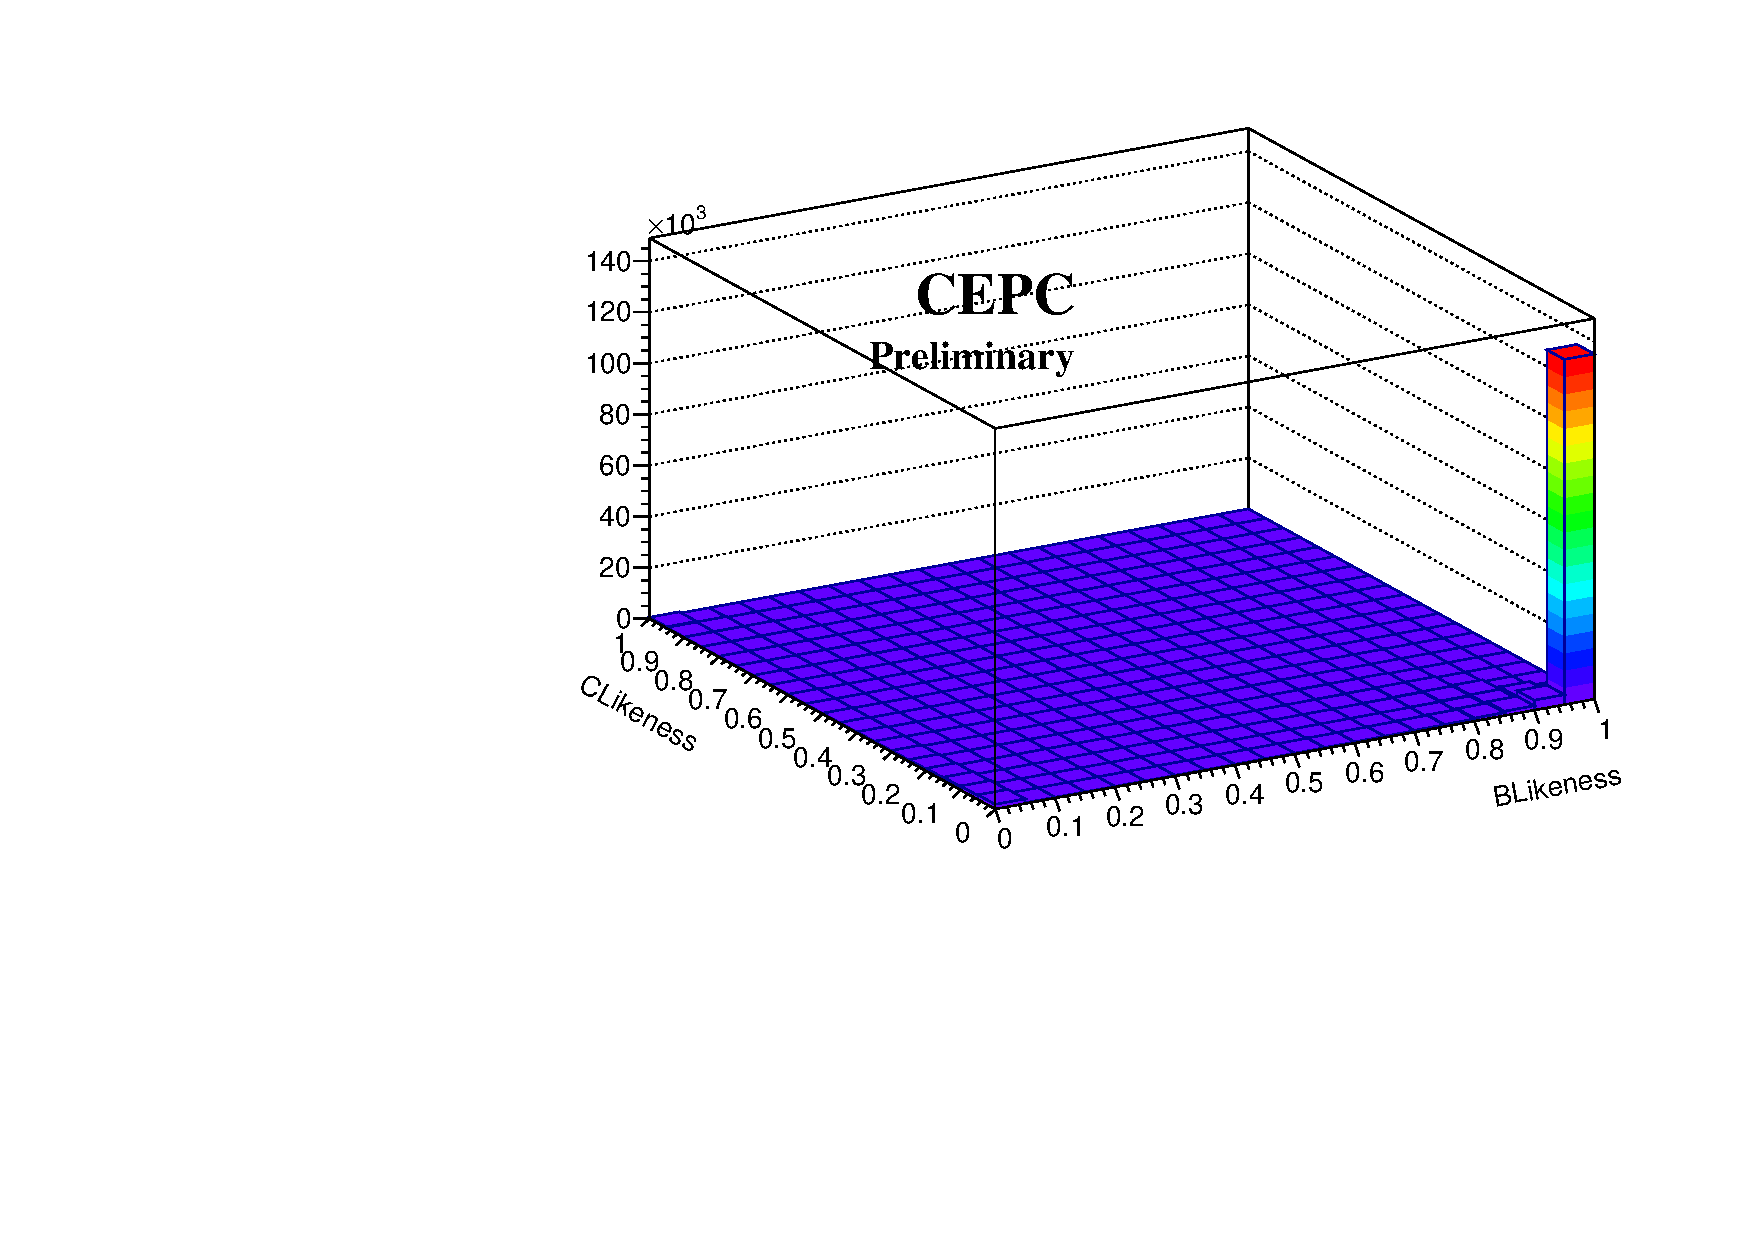
\includegraphics[width=\textwidth]{Template/qqh_bb.pdf}
%    \end{minipage}
%}
%\subfigure[]
%{ 
%   \begin{minipage}[b]{0.31\textwidth}
%   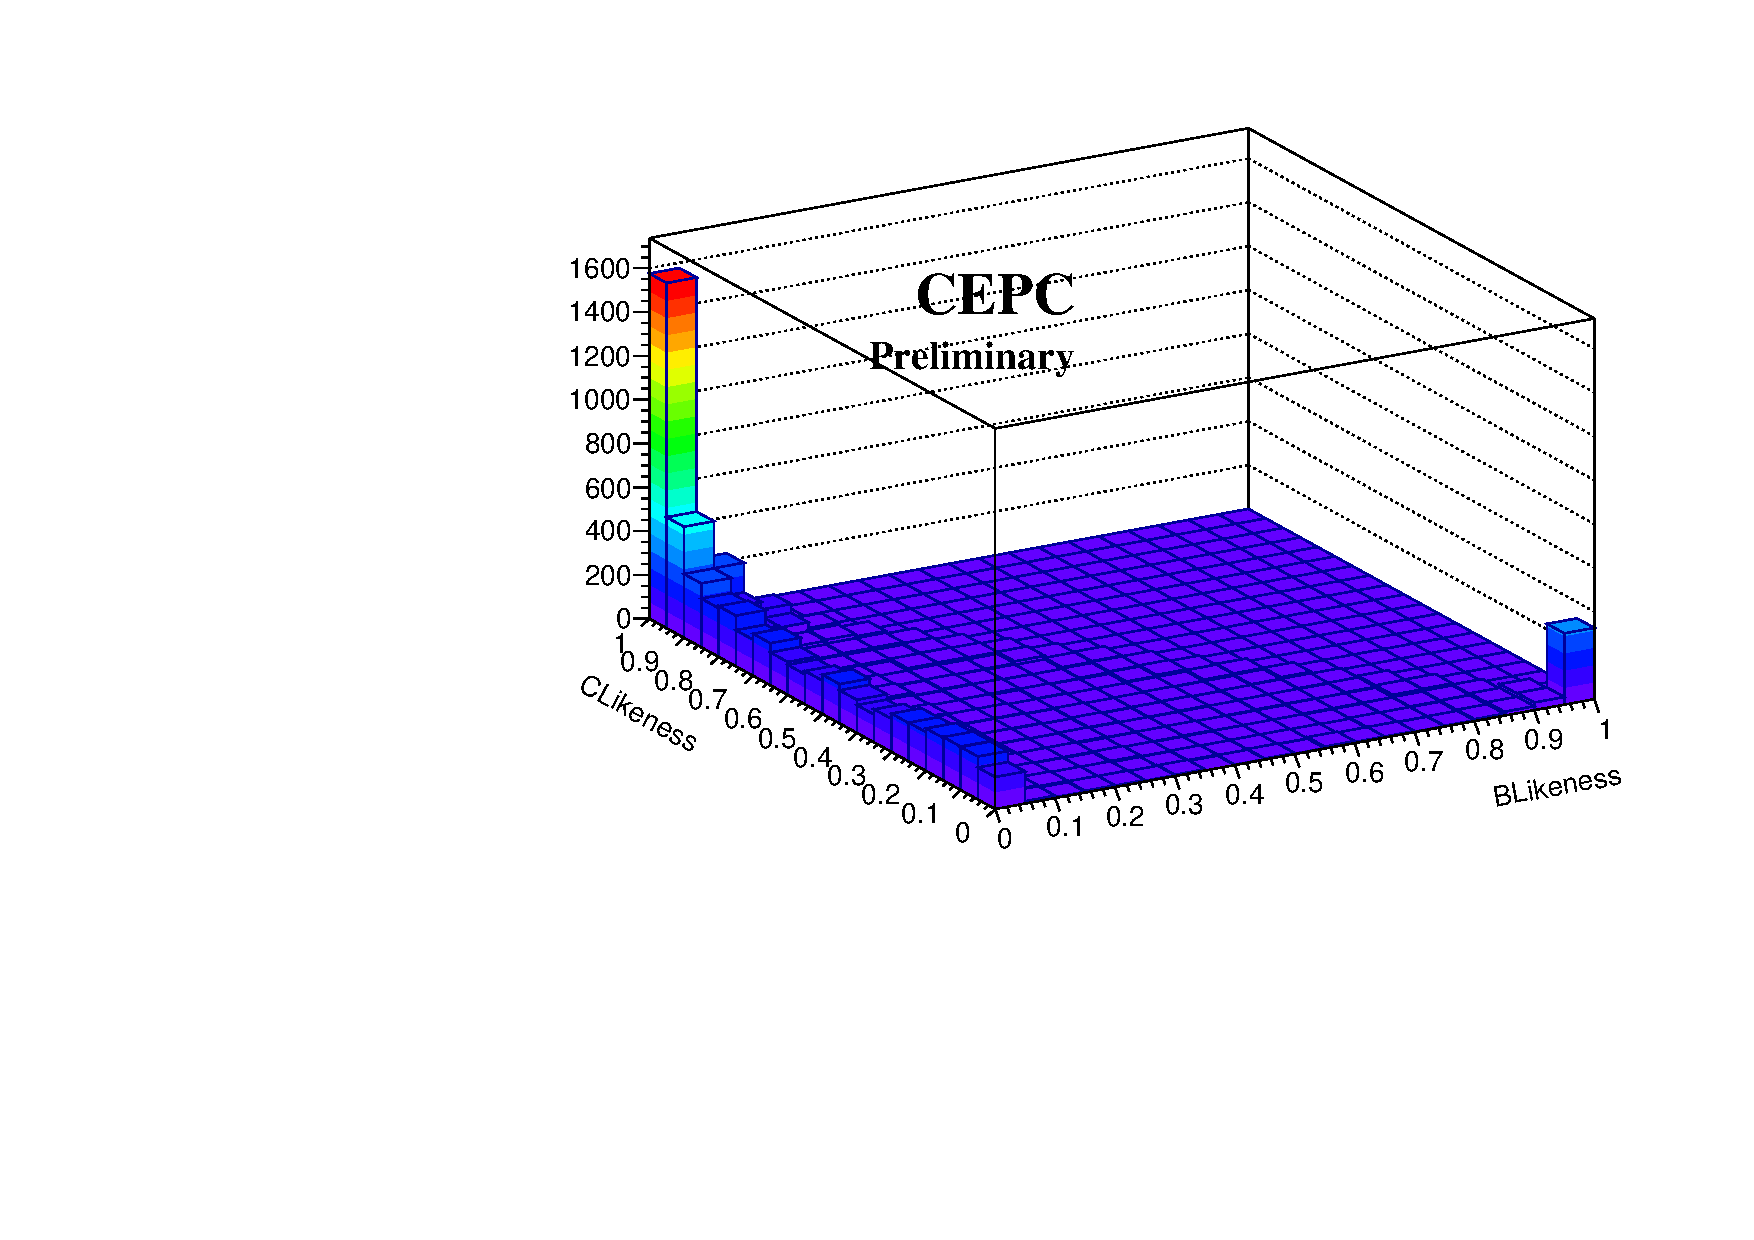
\includegraphics[width=\textwidth]{Template/qqh_cc.pdf}
%   \end{minipage}
%}
%\subfigure[]
%{
%    \begin{minipage}[b]{0.31\textwidth}
%    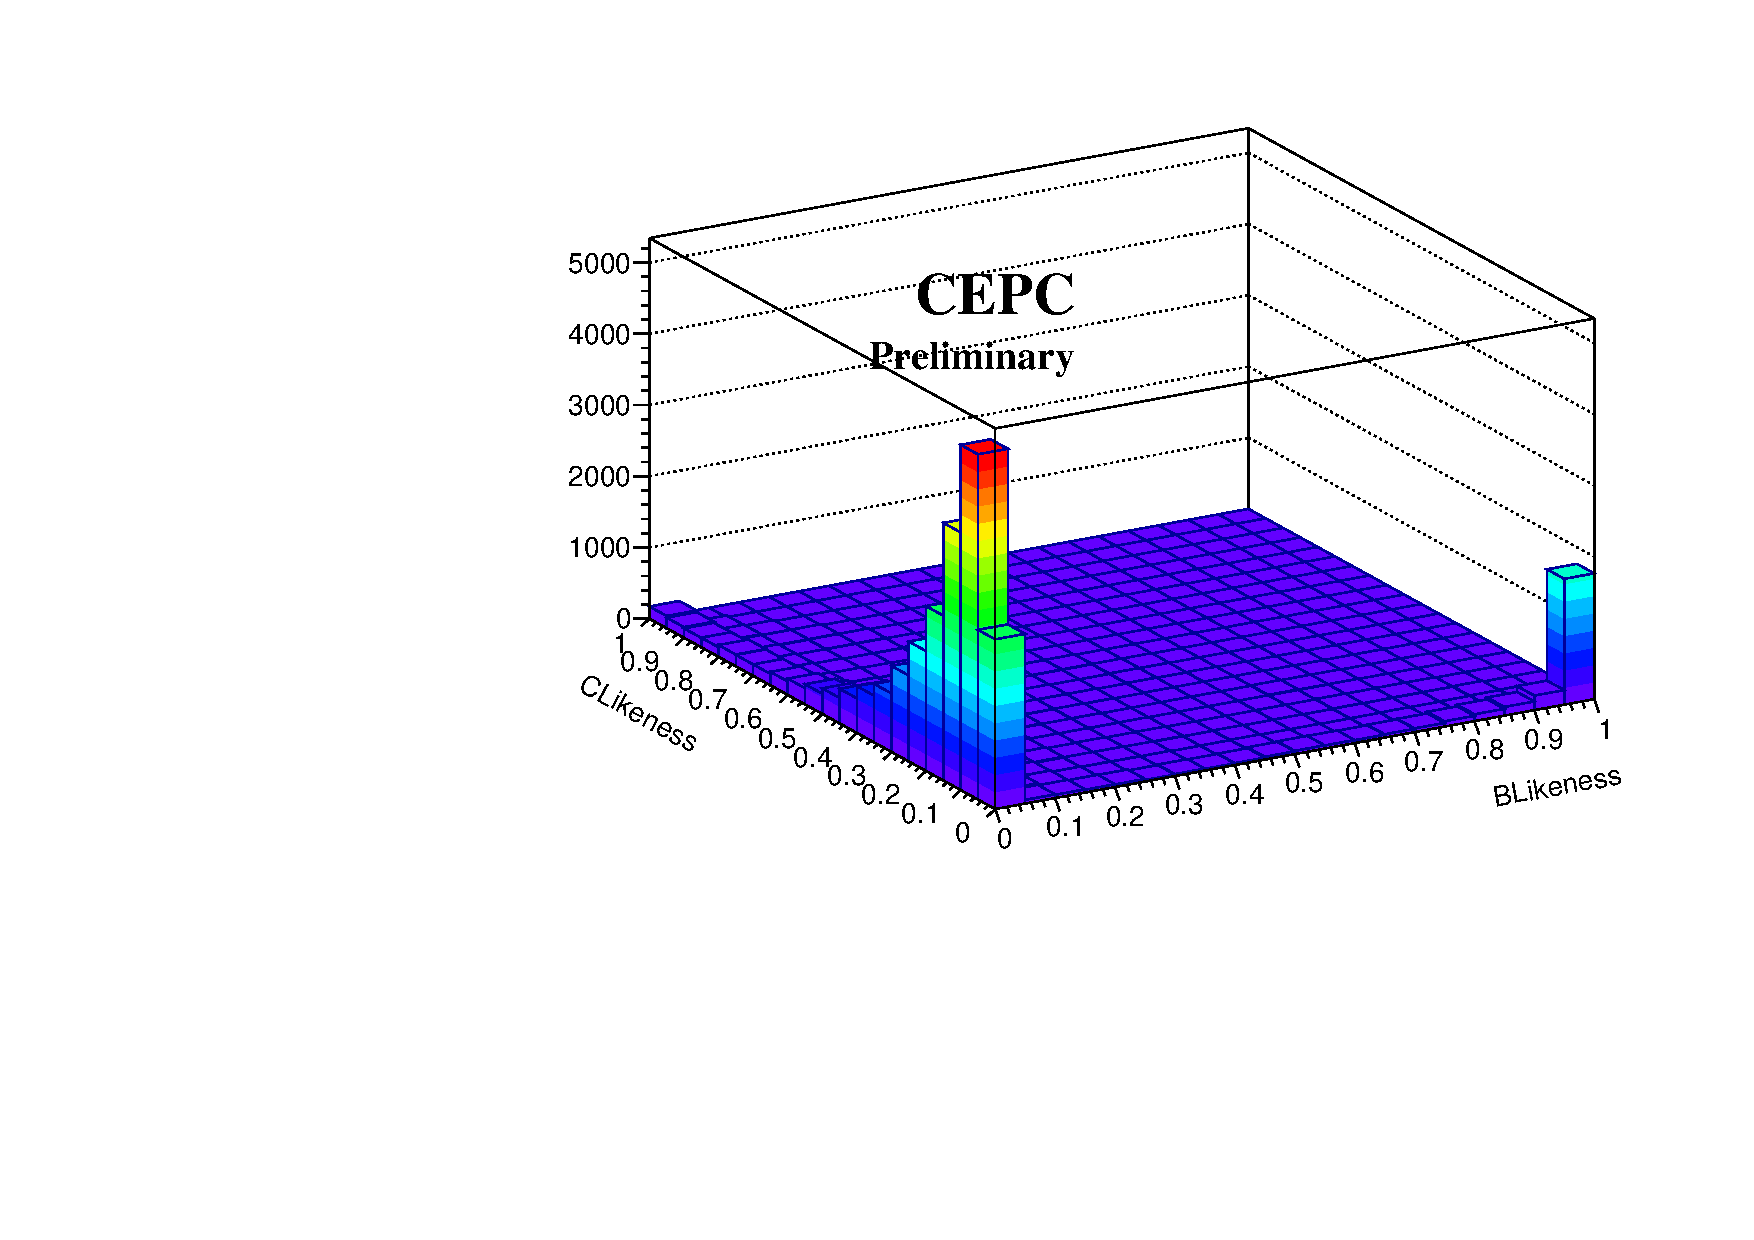
\includegraphics[width=\textwidth]{Template/qqh_gg.pdf}
%    \end{minipage}
%}
\caption{Template of signal events. 
%From top row to bottom row: templates of \eeh and \mmh; %\nnh and \qqh; 
From left column to right column: templates of $\Hboson\to\bpair$,$\Hboson\to\cpair$ and $\Hboson\to\gpair$.}
\end{figure}

%In the fit, the $\Hboson\to\bpair$,$\Hboson\to\cpair$ and $\Hboson\to\gpair$ combined events yield is set as free parameter, which is equal to $L\times \sigma_{ZH\to 4jets}$. The fraction of each of the 3 flavor finals states, say $f_b$,$f_c$ and $f_g$, contribute 2 independent free parameters\footnote{The renormalization requires $f_b+f_c+f_g = 1$, reducing the number of free parameter by 1.}. The shape of backgrounds are fixed. The background distribution was shown in figure \ref{fig:bkg_template}.
%
%\begin{figure}[!htpb]
%\label{fig:bkg_template}
%\centering
%\subfigure[]
%{
%  \begin{minipage}[b]{0.42\textwidth}
%  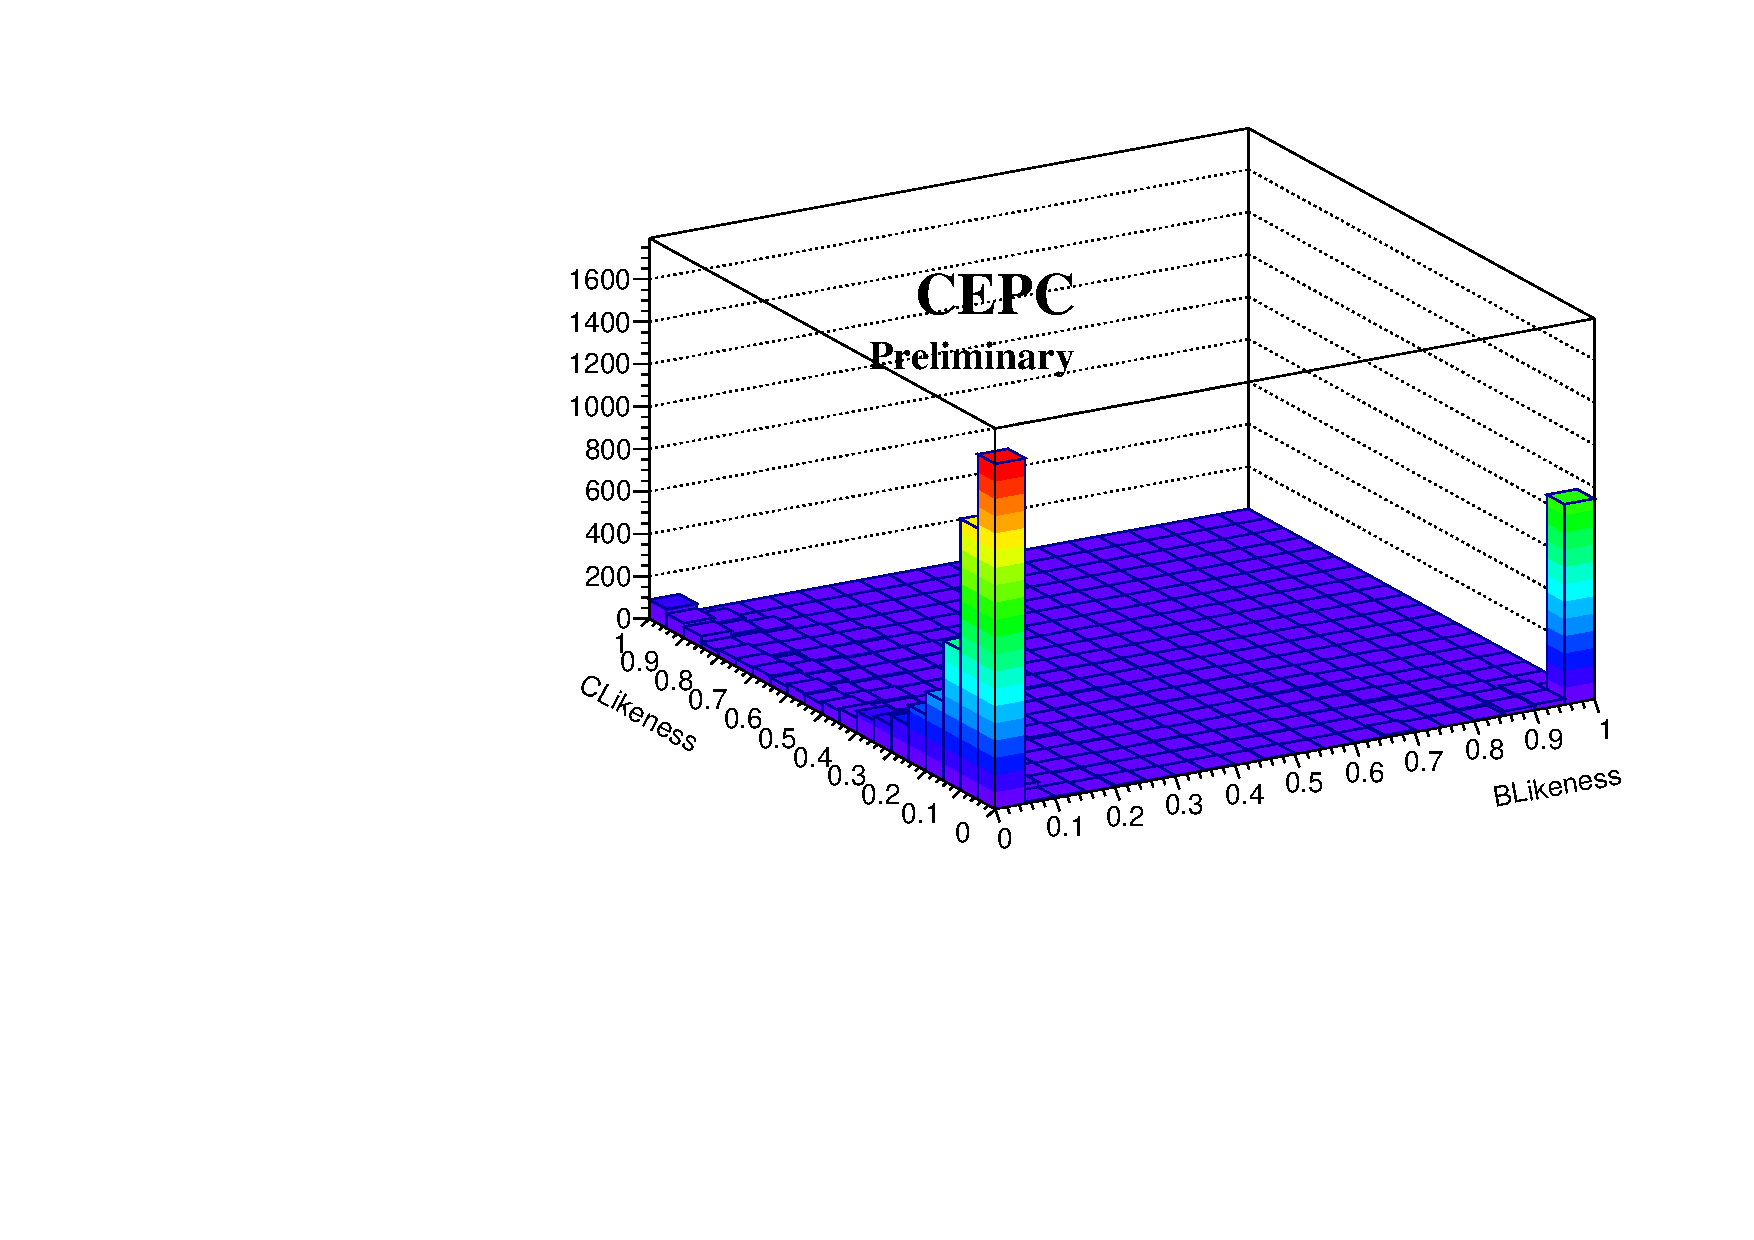
\includegraphics[width=\textwidth]{Template/eeh_bkg.pdf}
%  \end{minipage}
%}
%\subfigure[]
%{
%  \begin{minipage}[b]{0.42\textwidth}
%  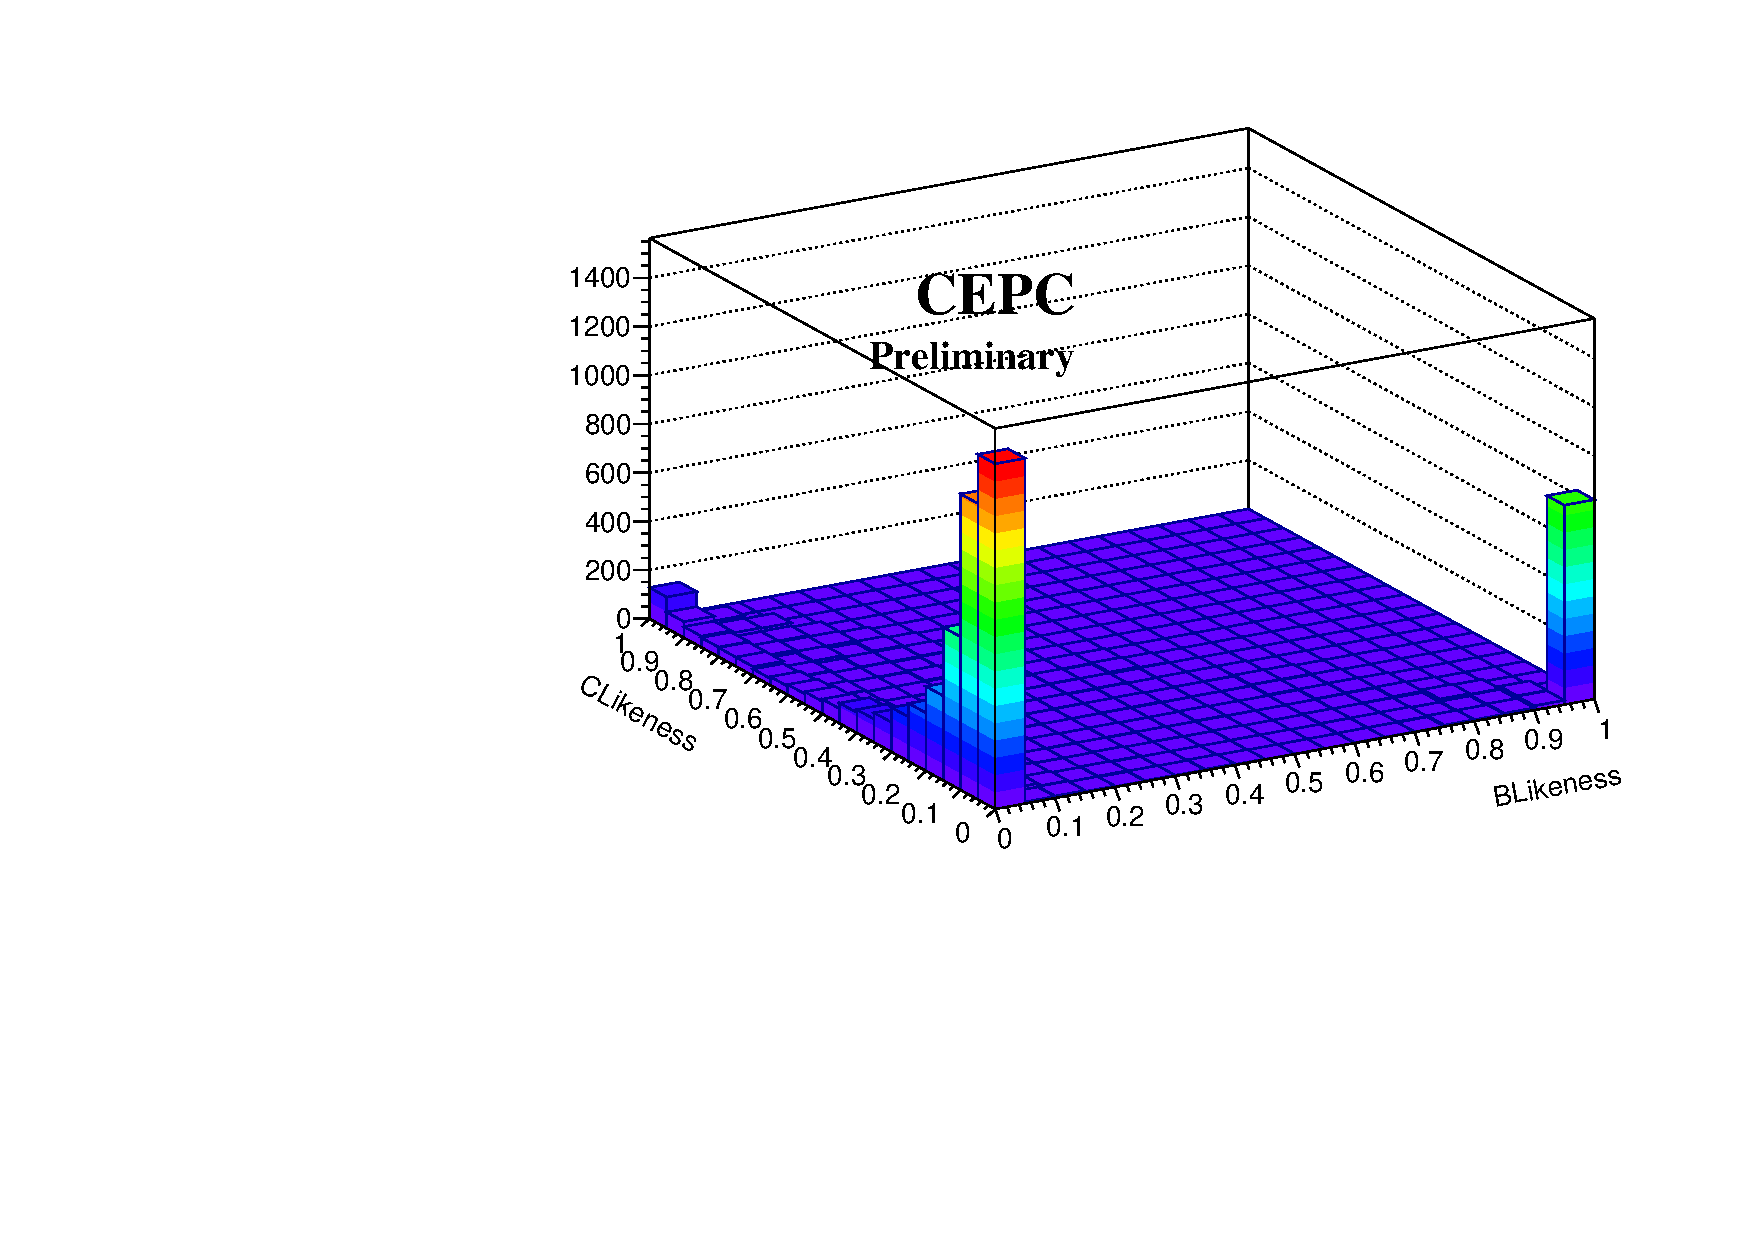
\includegraphics[width=\textwidth]{Template/mumuh_bkg.pdf}
%  \end{minipage}
%}
%%\subfigure[]
%%{ 
%%   \begin{minipage}[b]{0.42\textwidth}
%%   \includegraphics[width=\textwidth]{Template/nnh_bkg.pdf}
%%   \end{minipage}
%%}
%%\subfigure[]
%%{
%%    \begin{minipage}[b]{0.42\textwidth}
%%    \includegraphics[width=\textwidth]{Template/qqh_bkg.pdf}
%%    \end{minipage}
%%}
%\caption{Templates of background events in \eeh(top left) and \mmh(top right)channel.}
%\end{figure}


%\begin{figure}[htpb]
%\centering
%    \includegraphics[width=0.88\textwidth]{figures/c1.eps}
%\caption{ Distribution of $X_B-X_C$ for $H->bb$ (top left), $H->cc$(top right)m $H->gg$ and other $ffH$.
%}
%\label{fig:templates}
%\end{figure}


% To get the jet pair from higgs decay was determined by comparing the $\chi^2$ defined in formula \ref{for:chi2}. With a 21\% possibility to get wrong combination, this is not perfect. The mismatch of PFOs and jets degenerate the paring correct rate. The complication of QCD process and hadronization can significantly affect the correct rate of PFO jet matching:
% \begin{itemize}
% \item Gluon radiation: give rise to considerable charge in partons momentum.  
% \item Gluon splitting: causing a more complex final states with additional parton
% \end{itemize}
\subsection{Three dimension fit on flavor templtes and recoil mass}

\label{subsec:3D_fit}
A set of 3-dimension PDFs are defined by the production of the flavor PDF and recoil mass PDFs. 
\begin{equation}
PDF^{3D}(X_B,X_C,M_{recoil}) = PDF^{flavor}(X_B,X_C)\times PDF^{recoil\_mass}(M_{recoil})
\end{equation}
The recoil mass of \mmh events was described by a crystal ball function plus a double sided exponential function, while the recoil mass of background events are discribed by a second order Chebychev polynomial function; $PDF^{flavor}$ is the flavor PDFs defined in 
 \ref{subsec:templatefit}. 
 For signals, the crystal-ball distribution shape are assumed to be indepdent to different flavor final states from higgs decay, 
 and similarly the $ZZ$ semi-leptonic final states share the description of recoil mass spectrum. In fig \ref{fig:recoilmass_fit}, the recoil mass fit for the signal 
 and signal + background are presented. We can find the the perfect signal modeling are insured in the fit.\par
 \begin{figure}
 \label{fig: recoilmass_fit}
 \centering 
 \subfigure[]
{ 
   \begin{minipage}[b]{0.47\textwidth}
   \includegraphics[width=\textwidth]{Template/MuMu_recoil_sig_logscale.pdf}
   \end{minipage}
}
\subfigure[]
{
    \begin{minipage}[b]{0.47\textwidth}
    \includegraphics[width=\textwidth]{Template/MuMu_recoil_1D.pdf}
    \end{minipage}
}
\caption{ \mupair recoil mass fit . Left: \mmh only fit. Right: Signal+Background fit.}
 \end{figure}

 There are 4 parameters for crystal-ball shape and 2 parameters for polynomial, in addition, there are 9 parameters for signal and background 
 normalizations. 
 The shape parameters of recoil mass PDFs are free in the fit. 
 The normalization parameters for signals, $ZZ\to \mupair+\qpair$ are also float, while normalization parameters for $ZH\to ZWW^*$ and $ZH\to ZZ^*$ are fixed. Both shape and normalization parameters for other backgrounds are fixed. The shape of those minor backgrounds are taken from MC simulation in 
 the form of a 3-dimension histogram in $X_B$-$X_C$-$Recoil\_Mass$ space. 
  The parameters setting are illustrated in table \ref{tab:fit_3d_para}.\par
  \begin{table}\label{tab:fit_3d_para}
  \centering
  \begin{tabular}{r|c|c|c|c|c|c|c|c|c} \hline
              &\multicolumn{3}{|c|}{signal}&\multicolumn{2}{|c|}{$\llh$ background}   & \multicolumn{3}{|c|}{$ZZ$ semi-leptonic} & other background \\ \cline{2-9}
              & $\bpair$ & $\cpair$ & $\gpair$ & $WW^*$ &
                 $ZZ^*$  & $\leppair + \bpair$ &  $\leppair + \cpair$       &  $\leppair + \qpair$  &   \\ \hline
  Recoil mass shape  &    \multicolumn{5}{|c|}{Released}   &    \multicolumn{3}{|c|}{Released}  &   Fixed \\ \hline 
  Normalization      & R & R & R & F & F & R& R &R & F\\ \hline           
  \end{tabular}
  \caption{Parameters setting in the 3D-fit. The signal and $\llh$ backgrounds share the same recoil mass shape; the $ZZ$ semi-leptonic background share the same recoil mass shape. Other background's shape and normalization are fixed according to a 3-dimension histogram distribution. The 'R' and 'F' in last row stands for 'Released' and 'Fixed' respectively. }
  \end{table}

%\subsection{ToyMC test with templatefit}
%A ToyMC test was applied to evaluate the uncertainty from template fit. In this test, the template fit was done repeatly to the different datasets, in which events yields at each bin on the $X_B-X_C$ distribution are set to be random value according to Possion distribution. This test deomonstrate the unceratiny from the fit  due to data statistic fluctuation. The fit results for $\eeh$ and $\mmh$ are shown in figure \ref{fig:toymc_subchannel}. 
%
%\begin{figure}[!htpb]
%\centering
%\subfigure[]
%{
%     \begin{minipage}[b]{0.31\textwidth}
%     \includegraphics[width=\textwidth]{Template/toymc_eeh_bb.pdf}
%     \end{minipage}
%}
%\subfigure[]
%{
%     \begin{minipage}[b]{0.31\textwidth}
%     \includegraphics[width=\textwidth]{Template/toymc_eeh_cc.pdf}
%     \end{minipage}
%}
%\subfigure[]
%{
%     \begin{minipage}[b]{0.31\textwidth}
%     \includegraphics[width=\textwidth]{Template/toymc_eeh_gg.pdf}
%     \end{minipage}
%}
%\subfigure[]
%{
%     \begin{minipage}[b]{0.31\textwidth}
%     \includegraphics[width=\textwidth]{Template/toymc_mumuh_bb.pdf}
%     \end{minipage}
%}
%\subfigure[]
%{
%     \begin{minipage}[b]{0.31\textwidth}
%     \includegraphics[width=\textwidth]{Template/toymc_mumuh_cc.pdf}
%     \end{minipage}
%}
%\subfigure[]
%{
%     \begin{minipage}[b]{0.31\textwidth}
%     \includegraphics[width=\textwidth]{Template/toymc_mumuh_gg.pdf}
%     \end{minipage}
%}
%%\subfigure[]
%%{
%%     \begin{minipage}[b]{0.31\textwidth}
%%     \includegraphics[width=\textwidth]{Template/toymc_nnh_bb.pdf}
%%     \end{minipage}
%%}
%%\subfigure[]
%%{
%%     \begin{minipage}[b]{0.31\textwidth}
%%     \includegraphics[width=\textwidth]{Template/toymc_nnh_cc.pdf}
%%     \end{minipage}
%%}
%%\subfigure[]
%%{
%%     \begin{minipage}[b]{0.31\textwidth}
%%     \includegraphics[width=\textwidth]{Template/toymc_nnh_gg.pdf}
%%     \end{minipage}
%%}
%%\subfigure[]
%%{
%%     \begin{minipage}[b]{0.31\textwidth}
%%     \includegraphics[width=\textwidth]{Template/toymc_qqh_bb.pdf}
%%     \end{minipage}
%%}
%%\subfigure[]
%%{
%%     \begin{minipage}[b]{0.31\textwidth}
%%     \includegraphics[width=\textwidth]{Template/toymc_qqh_cc.pdf}
%%     \end{minipage}
%%}
%%\subfigure[]
%%{
%%     \begin{minipage}[b]{0.31\textwidth}
%%     \includegraphics[width=\textwidth]{Template/toymc_qqh_gg.pdf}
%%     \end{minipage}
%%}
%\caption{Toy MC test result in terms of signal strength and uncertainty from template fit. The signal strength from template fit in each channel for each higgs hadronic decay is presented. Plots in each row are from the same channel, from top row to bottom row are : \eeh, \mmh, \nnh and \qqh; plots in each column are from the same higgs decay mode, from left to right column are $H\rightarrow \bpair$, $H\rightarrow \cpair$ and $H\rightarrow \gpair$.}
%\label{fig:toymc_subchannel}
%\end{figure}


\section{Validtion of the Template Fit Method}
A delicate flavor tagging commissioning is required to validate the template fit method. The discrepancy between data and monte carlo in template distribution will lead to biased fitting results. 
Thus it is necessary to apply the tempalte fit to a control sample, and estimate the results in terms of the bias in each flavor components. 
In this section, we are not trying to directly esimate that bias since we have no collision data, but to demonstrate  feasibility of the procedure of the validation. \\
The semi-leptonic $ZZ$ events can be selected as the control sample. There are several advantage to do so:
\begin{itemize}
\item The cross section of $ZZ$ events is large. There will be about 1.1 million semi-leptonic $ZZ$ channel with $\mupair\qpair$ and $\nu\bar{\nu}\qpair$ each, and over 1.6 million events with $\elpair\qpair$ events.
\item The hadonic $Z-$decay provide abundant $\bpair$ and $\cpair$ events
\item The signiture of $ZZ$ events is very clear, by which purity of the control sample can be guaranteed 
\item The kinematic feature of jets in the $ZZ$ semi-leptonic jets is similar to that in signal 
\end{itemize}
The $ZZ$ events was selected in $ZZ\to\mu^{+}\mu{-}q\bar{q}$ channel. The invariant mass of $\mupair$, jet-pair and the $\mupair$ recoil mass are required in $Z$-resonance region, which can be seen in figure \ref{fig:ZZ_mumuqq_valid}. The event yields of $ZZ\to\mu^{+}\mu{-}q\bar{q}$ and other process are shown in tabel \ref{tab:ZZ_mumuqq_valid}.
\begin{figure}[!htpb]
\label{fig:ZZ_mumuqq_valid}
\centering
\subfigure[]
{
  \begin{minipage}[b]{0.31\textwidth}
  \includegraphics[width=\textwidth]{Validation/mumuh/mumu_inv.pdf}
  \end{minipage}
}
\subfigure[]
{
  \begin{minipage}[b]{0.31\textwidth}
  \includegraphics[width=\textwidth]{Validation/mumuh/mumu_recoil.pdf}
  \end{minipage}
}
\subfigure[]
{
  \begin{minipage}[b]{0.31\textwidth}
  \includegraphics[width=\textwidth]{Validation/mumuh/jj_inv.pdf}
  \end{minipage}
}
\caption{The invariant mass of $\mupair$(left), the recoil mass of $\mupair$ and the invariant mass of jet pair in $ZZ$ control sample}
\end{figure}

\begin{table}
\label{tab:ZZ_mumuqq_valid}
\begin{tabular}{r|c|c|c|c}
             &   $ZZ$ semi-leptonic     &     $W^{+}W^{-}$ semi-leptonic     &       $\mmh$     &   $\qqh$   \\ \hline
 75 GeV$<M_{\mupair}<$105 GeV
            &       193.3k              &      412.2     &   25.96k   & 366.68      \\ \hline
  80 GeV$<M_{\mupair recoil}<$110 GeV
            &       157.4k              &      132.9     &   13.99    &  5.01 \\ \hline
   75 GeV$<M_{jj}<$100 GeV 
            &       124.1k              &       8.41     &   2.51     &  1.00\\ \hline 
  Purity    &  \multicolumn{4}{c}{99.99\%}     \\ 
               
\end{tabular}
\caption{Events yields of semi-leptonic ZZ events and other dominant process.} 
\end{table}
  
  
 

 \section{Results}\label{sec:results}
 To extract the signal strength from all the four sub channels, a combination template fit was applied.
 This fit concentrate also makes use of $X_B-X_C$ distribution in each channel. 
 The combined log-likelihood is defined as the sum of that in each sub channel.
 The free parameters are the same as that in the fit of each channel, described in \ref{subsec:flavortagging}. 
 The fraction of each flavor are set as common parameter,while the over all hadronic yields in each channel are set as indepedent parameter. The combined fit results are shown in figure \ref{fig:combined_fit}. 
 
\begin{figure}[!htpb]
\label{fig:combined_fit}
\centering
\subfigure[]
{
  \begin{minipage}[b]{0.31\textwidth}
  \includegraphics[width=\textwidth]{Template/toymc_combined_bb.pdf}
  \end{minipage}
}
\subfigure[]
{
  \begin{minipage}[b]{0.31\textwidth}
  \includegraphics[width=\textwidth]{Template/toymc_combined_cc.pdf}
  \end{minipage}
}
\subfigure[]
{ 
   \begin{minipage}[b]{0.31\textwidth}
   \includegraphics[width=\textwidth]{Template/toymc_combined_gg.pdf}
   \end{minipage}
}
\caption{Combined template fit results of signal strength for $H\rightarrow \bpair$, $H\rightarrow\cpair$ and $H\rightarrow\gpair$ process.}
\end{figure}
 
%After the cutflow(except for the $\chi^2$ cut in the last step) being applied, the template fit was implemented to the sample consist of $qqH\to bb/cc/gg$ and the background events. The fast simulation background sample don't have vertex reconstructed so there is no way to apply flavor tagging on it. Thus currently the background only contains the fully reconstructed  higgs production sample, including 75413 $\qqbar\Hboson\to\qqbar\Wboson\Wboson$ events, 10091 $\qqbar\Hboson\to\qqbar\Zzero\Zzero$ events, 8444 $\qqbar\Hboson\to\qqbar\tautau$ events and 7780 $\nnbar\Hboson\&\leplep\Hboson$ events. The fitted sample distribution in $X_B-X_C$ coordinate is shown in figure \ref{fig_data}. The fitting result is shown in table \ref{tab:fit_result}
%\begin{figure}[!htpb]\label{fig:fit_data}
%\centering
%    \includegraphics[width=0.88\textwidth]{figures/c1_n2.eps}
%\caption{ Distribution of $X_B-X_C$ fitted sample}
%\label{fig:templates}
%\end{figure}
%
%\begin{table}[h]
%\begin{center}
%\begin{tabular}{cccccccc}
%\hline
%\hline
%Channel		&	data	&	fit	&	sigma	&	sigma/fit&	bias	&	bias/data	&	template	\\
%\hline
%$\bbbar$	&	263.5k	&	261.2k	&	699	&	0.266\%	&	2357	&	0.894\%		&	data itself	\\\hline
%$\ccbar$	&	12.22k	&	12.95k	&	574	&	4.43\% 	&	737	&	6.03\%		&	data itself	\\\hline
%gg		&	41.06k	&	45.93k	&	1359	&	2.96\% 	&	4875	&	11.9\%		&	data itself	\\\hline
%\multirow{2}{2cm}{$\ffbar\Hboson$ background}&\multirow{2}{*}{102.5k}&\multirow{2}{*}{99.28k}&\multirow{2}{*}{2069}&\multirow{2}{*}{2.08\% }&\multirow{2}{*}{-3255}&\multirow{2}{*}{-3.18\%}&\multirow{2}{*}{\minitab[c]{$\nnbar\Hboson\&\qqbar\Hboson$:data itself \\ the others: other events}} \\\\
%\hline
%\hline
%\end{tabular}
%\caption{Template fit results, and the deviation to the true value}
%\end{center}
%\label{tab:fit_result}
%\end{table}
%The outcome of the fit shows significant deviation from true event yields for $H\to gg$ and $ffbarH$, while 
%the fitted $H\to bbar$ and $H\to ccbar$ event yields is relatively reasonable.  Strong correlation between $H\to gg$ and $ffH$ from fitting can be found in table \ref{tab:fit_matrix}, largely due to resemblance between the distribution of these two process shown in bottom plots in figure \ref{fig:templates} and cause considerable deviation in the fitting. Thus a predetermination of the $ffH$ fraction can significantly reduce the uncertainty of $H \to gg$ fraction from fitting.
%\begin{table}[h]
%\begin{center}
%\begin{tabular}{|c|c|c|c|c|c|c|c|}
%\hline
%\hline
%Channel	&	$\bbbar$	&	$\ccbar$	&	$gg$		&	$\ffbar\Hboson$\\\hline
%$\bbbar$	&	1.000	&	0.280  	&	0.332	&	-0.453		\\\hline
%$\ccbar$	&	0.280  	&	1.000  	&	0.629 	&	-0.774		\\\hline
%$gg$		&	0.332  	&	0.629  	&	1.000 	&	-0.927		\\\hline
%$\ffbar\Hboson$&0.453 	&	-0.774	&	-0.927  	&	1.000		\\\hline
%\hline
%\hline
%\end{tabular}
%\caption{Template fit correlation matrix}
%\end{center}
%\label{tab:fit_matrix}
%\end{table}

\section{Conclusion}\label{sec:summary}
The $ZH\to \mupair + \bpair/\cpair/\gpair$ brach ratio measurement is done with 5000 \ifb $\elpair$ collsion at $\sqrt{s} = $ 250 \GeV in CEPC experiment, demonstrating the capability of the CEPC experiment in Higgs yukawa coupling with its excellent PFA and flavor tagging performance. 
The statistic uncertainty for $H\to \bpair$, $H\to\cpair$ and $H\to\gpair$ branch fraction is esitmated as 1.1\%, 10.5\% and 5.4\%, while the systematic uncertainty of the 3 channels are $^{+0.73\%}_{-0.36\%}$, $^{+6.1\%}_{-6.2\%}$ and $^{7.6\%}_{-7.7\%}$. This is the first time to study $ZH\to \mupair + \bpair/\cpair/\gpair$ with fully 
simulation sample as well as taking into account the systematic unceraties. The results are consistent with the corresponding results in CEPC-SppC pre-CDR\cite{CEPC_preCDR} in terms of the statistic uncertainties. The results in this document will be incorporated with 
the study of $H\to/\bpair/\cpair/\gpair$ from other channels, like $qqH$ and $\nu\nu H$.\par
%The combination template fit from \eeh,\mmh,\nnh and \qqh $ $evaluate the uncertainty of $H\rightarrow \bpair$, $H\rightarrow \cpair$ and $H\rightarrow \gpair$ to be 0.27\%, 3.2\% and 1.6\%, reflecting the statistic uncertainty with 5000 \ifb integral luminosity data taken at $\sqrt{s} = $250 \GeV at CEPC. These results are done with all the backgrounds and signals from full simulation, and is consistent to the number estimated in pre-CDR. The precision of $H\rightarrow \bpair$ is mainly constrained by \qqh $ $channel, while the other two hadronic decay modes are mainly constrained by \nnh$ $ channel. In \qqh$ $ channel, $H\rightarrow \gpair/\cpair$ suffered from huge backgrounds from hadronic diboson process, and the mis-combination of jet pair degenerate the percision. To solve these problem, it is necessary to optimize the detector and reconstruction performance, which future work should concentrate on.

\clearpage
\pagebreak
\newpage

%\appendix
\section{Jet pairs from $\Hboson$ and $\Zzero$ invariant mass }
The width of invariant mass of jet pairs from a signal boson can be affected by the following facts:
\begin{itemize}
\item The Breit-Weigner structure of bosons. This facts can be ignored in higgs decay (the width is esitmated as a few MeV) 
\item PFOs energy resolution, which is around 3\%.
\item Missing energy and momentum due to semi-leptonic decay
\item Missing energy and momentum due to soft radiation, which produces low energy objects missing from detection.
\item Mis-match between the PFO and the jets. 
\end{itemize}
To estimate the width from higgs decay, a $\Zzero\Hboson\to \mu^+\mu^- \qqbar/gg$ sample is used.
\clearpage
\section{Event filter for $\qqbar$ events}
 The $\qqbar$ process frequently happen with additional gluon radiated from primary quarks, and form one or more jets, rising the probablity of passing the event selection. This fact can be demonstrate by comparing the $y_{34}$ value distribution of the $\qqbar$ events with and without hard gluon radiation, see figure\ref{fig:y34_filter}. When a quark emit a gluon with $p_T>$20 GeV, outside of a $\Delta R=$0.7 cone from the residule quark after emission, and carry more than 25\% of the energy of the quark before emssion, a hard gluon radiation is tagged to this event. Gluon radiation is also considered by looking for if there is quarks from gluon. The emitted gluon and the quarks from gluon radiation are put in a parton list, in which the candidates as the source of jets before hadronization. A parton in the list is assumed to be the origin of a jet if it has energy larger than 20 GeV. Thus the parton multiplicity in terms of jets can be larger than the primary parton multiplicity.\par
 
 
Due to the huge cross section of $\qqbar$ events(about 50 pb in total), generating such backgrounds yielding comparable equivalent integral luminosity as that for other backgrounds (~ 5000 fb$^{-1}$) is beyond reality. However most of the $\qqbar$ events passing the selection are those with hard gluon radiation, as shown in table \ref{tab:filter}, so one can make a filter in generation level to reject the events without hard gluon radiation. 
 

\begin{figure}[!htpb]\label{fig:fit_data}
\centering
    \includegraphics[width=0.65\textwidth]{figures/y34_compare.eps}
\caption{ $y_{34}$ distribution of events with different parton multiplicity in $\qqbar$ sample}
\label{fig:y34_filter}
\end{figure}

In addition, we have \emiss cut and $\qqbar$ has a high rate to emit a high energy photon very close to the beam direction and has a large chance to escape from detection. By requring the missing energy (of the $\qqbar$ system) smaller than a threshold can further reduce the statistics needed to be simulated. The combined filter is applied in the $\qqbar$ full simulation.

\begin{table}[!htpb]
\centering
\begin{tabular}{|c|c|c|c|}\hline
   NParton     &    $\leq 2$     &   3      &    4       \\ \hline
 Event Yields  &    202.75M      &  38.01M  &  5.44M     \\ \hline
 \emiss$\leq$ 85 GeV
               &    85.38M       &  21.23M  &  4.06M     \\ \hline
 \tabincell{c}{Jet quality\\ $y_{34}\leq$0.02}
              & \tabincell{c}{37.2k  \\4.18\%}
                                 & \tabincell{c}{233.1k \\26.18\%}
                                            &  \tabincell{c}{619.8k \\ 69.64\%} \\ \hline
\end{tabular}
\caption{The event yields of $\qqbar$ events with 2,3 and 4 partons before and after filter. The filter has efficiency around 10\% and 95\% of events passing the event selection are those which pass the filter.}
\label{tab:filter}
\end{table}

\clearpage
\section{TMVA in the application of flavor tagging}
To distinguish signal and background, the TMVA has been done using the BDT method\cite{BDT}. Signal and the $\ffbar\Hboson$ background are used to train the BDT. The input variables are shown in Figure 1.The distribution of BDT is shown in Figure 2.\par
\begin{figure}[h]
  \centering
  \includegraphics[width=15cm,height=8cm]{inputvar.eps}
  \includegraphics[width=5cm,height=4cm]{inputvar2.eps}
  \caption{The input variables}
\end{figure}
In  Figure 1, the variable Hmass is the invariant mass of the Higgs jets which are regarded as the Higgs decay product by minimizing the $\chi^2$; Zmass is the invariant mass of the other two jets, Z jets; Hjetsangle is the cosine of the Higgs jets' intersection angle; Zjetsangle is the cosine of the Z jets' intersection angle.\par
\begin{figure}[h]
  \centering
  \includegraphics[width=11cm,height=8cm]{distribution.eps}
  \caption{The BDT distribution}
\end{figure}
It's obvious that if we execute cut $BDT>0.04$, we will get a ideal significance. However, we cannot do this because we will loss many events of the gg channel, which can be seen in Figure 3.\par
\begin{figure}[h]
  \centering
  \includegraphics[width=11cm,height=8cm]{gg_bkg.eps}
  \caption{The BDT of gg distribution}
\end{figure}
So a new thinking occurs: we can train 3 kinds of BDT to distinguish 3 kinds of signal respectively. The branch ratio will obtained by carry out the template fit of BDT. This will be the next step.
\clearpage

\section{Tag counting method in the application of flavor tagging}
The tag counting method is implemented in B-tagging calibration using $\ttbar$ events in ATLAS 
experiment\cite{ATLAS_CSC}. Mathematically it can also used to reversly to resolve the fraction of events with various components. \par
The tag counting method is based on:
\begin{equation}\label{for:tagcounting}
<N_n> = (L\times\sum\limits_{c=1}^s(\sigma_c \times A_{c,\mathrm{pre-tag}}))\times\sum\limits_{i,j,k}F_{ijk}\sum\limits_{i^\prime+j^\prime+k^\prime=n}C^{i^\prime}_i\epsilon_b^{i^\prime} (1-\epsilon_b)^{i-i^\prime}C^{j^\prime}_j\epsilon_c^{j^\prime} (1-\epsilon_c)^{j-j^\prime}C^{k^\prime}_k\epsilon_l^{k^\prime} (1-\epsilon_l)^{k-k^\prime}
\end{equation}
in which $<N_n>$ is the expected observed events number with $n$ jets passing b-tagging; $L$ is integral luminosity and $\sigma_c$ and $A_{c,\mathrm{pre-tag}}$ are the cross section and acceptance before applying the flavor tagging for channel $c$;factor $F_{ijk}$ is defined as the fraction of events with $i$ b-jets, $j$ c-jets and $k$ light jets;  $C^{i^\prime}_i$ is the arragement number: $\dfrac{i!}{i^\prime!(i-i^\prime)!}$; the prime subscript corresponding to the tagged jets of given flavor; and $\epsilon_b$,$\epsilon_c$ and $\epsilon_l$ stand for average the tagging efficiency for b, c and light jets.\par
By requiring 4 jets in final states, there are 15 $F_{ijk}$ to determine\footnote{There are 14 independent $F$ values due to the normalization relation $\sum\limits_{i,j,k}F_{ijk}=1$}. In $\Zzero\Hboson\to \qqbar + bb/cc/gg$ sample, the $F_{ijk}$ are listed in table \ref{tab:fijk}. It can be seen that $F_{400}$, $F_{202}$ and $F_{220}$ are signficantly larger than the others thus they have higher priority to be determined.  We can construct a log-likelihood via:
\begin{equation}\label{for:tagcounting_likelihood}
\log{L} = \sum\limits_{i=0}^4 Possion(<N_i>,N_{i,observed})
\end{equation}
By minimizing $-\log{L}$, one can get the number of $F_{ijk}$ of interest. Moreover, tagging efficiency like $\epsilon_b$ can also be set as free parameters for fitting.

\begin{table}[!htpb]
\centering
\begin{tabular}{|c|c|c|c|c|c|}\hline
               & $N_{cjets}=4$ & $N_{cjets}=3$ & $N_{cjets}=2$ & $N_{cjets}=1$ & $N_{cjets}=0$ \\ \hline 
 $N_{bjets}=4$ &    -          &      -        &      -        &      -        &   0.186  \\ \hline
 $N_{bjets}=3$ &    -          &      -        &      -        &     0.0192    &   0.0846 \\ \hline
 $N_{bjets}=2$ &    -          &      -        &     0.125     &3.9$\times10^{-5}$& 0.04232 \\ \hline
 $N_{bjets}=1$ &    -          & 6.75$\times10^{-3}$&6.90$\times10^{-6}$& 0    &   0.026  \\ \hline
 $N_{bjets}=0$ &7.02$\times10^{-3}$&4.08$\times10^{-3}$&0.0343 &6.71$\times10^{-3}$ & 0.0777\\ \hline   

\end{tabular}
 \caption{$F_{ijk}$ in $\Zzero\Hboson\to \qqbar + bb/cc/gg$ sample.}
 \label{tab:fijk}
\end{table}

Before applying the fit to get $F_{ijk}$, we did an input/output test in $\Hboson\Zzero\to \qqbar \bbbar/\ccbar/gg$ sample. The tagging efficiency was calculated from all the jets in the sample, then we compare $N_n$ from formula \ref{for:tagcounting} and $N_{n,observed}$. The result is listed in table \ref{tab:tagcounting_io}. Serious deviation was found especially for $F_2$ and $F_3$. This might be due to the average tagging efficiency is not independant to the flavor components, thus formula one can not be validated. 
\begin{table}
\centering
\begin{tabular}{|c|c|c|c|c|c|}\hline
            &   $F_0$     &    $F_1$     &   $F_2$      &    $F_3$       &    $F_4$    \\ \hline
$N_{n,observed}$       
            &    0.136    &   0.221      &   0.475      &     0.096      &     0.072   \\ \hline
$<N_n>$     &    0.142    &   0.252      &   0.386      &     0.156      &     0.064   \\ \hline              
\end{tabular}
\caption{The obvserved and calculated(according to formula \ref{for:tagcounting}) event number with cerntain tagged jets multiplicity. $F_i$ is defined as the fraction of events with $i$ jets tagged.}
\label{tab:tagcounting_io}
\end{table}
\clearpage 

\bibliographystyle{cepcBibStyleWoTitle}
\bibliography{instructions}

\end{document}
